% =============================================================================
%  MSc Project Report
%  An Intelligent Data Analytics and Machine Learning Framework for
%  Predictive Business Decision-Making: A Dan Cake Bangladesh Case Study
%
%  Compile:  pdflatex main -> bibtex main -> pdflatex main -> pdflatex main
%            (or simply upload the whole 'report' folder to Overleaf)
%  Numbers in the text come from generated/numbers.tex and tables from tables/,
%  both written by `python run_pipeline.py`. Do not type results by hand.
% =============================================================================
\documentclass[12pt,a4paper,oneside]{report}

% ---------------------------------------------------------------- packages
\usepackage[T1]{fontenc}
\usepackage[utf8]{inputenc}
\usepackage{lmodern}
\usepackage[margin=2.5cm,left=3cm]{geometry}
\usepackage{setspace}\onehalfspacing
\usepackage{graphicx}
\usepackage{booktabs,tabularx,longtable,array,multirow}
\usepackage{amsmath,amssymb}
\usepackage{xcolor}
\usepackage{caption}\captionsetup{font=small,labelfont=bf,skip=6pt}
\usepackage{float}
\usepackage{adjustbox}
\usepackage{enumitem}
\usepackage{xspace}
\usepackage{listings}
\usepackage{tikz}\usetikzlibrary{arrows.meta,positioning,shapes.geometric,shapes.multipart,fit,backgrounds}
\usepackage{fancyhdr}
\usepackage{titlesec}
\usepackage[round,authoryear]{natbib}
\usepackage[hidelinks]{hyperref}
\usepackage[nameinlink,capitalise]{cleveref}

\definecolor{brand}{HTML}{1F4E79}
\definecolor{accent}{HTML}{C55A11}
\definecolor{codebg}{HTML}{F5F7FA}
\titleformat{\chapter}[display]{\normalfont\huge\bfseries\color{brand}}{\chaptertitlename\ \thechapter}{12pt}{\Huge}
\titlespacing*{\chapter}{0pt}{-10pt}{24pt}
\titleformat{\section}{\normalfont\Large\bfseries\color{brand}}{\thesection}{1em}{}
\titleformat{\subsection}{\normalfont\large\bfseries}{\thesubsection}{1em}{}
\setlength{\headheight}{15pt}
\pagestyle{fancy}\fancyhf{}\fancyhead[L]{\small\nouppercase{\leftmark}}\fancyfoot[C]{\thepage}
\renewcommand{\headrulewidth}{0.4pt}
\fancypagestyle{plain}{\fancyhf{}\fancyfoot[C]{\thepage}\renewcommand{\headrulewidth}{0pt}}
\lstset{basicstyle=\ttfamily\footnotesize,backgroundcolor=\color{codebg},frame=single,rulecolor=\color{gray!40},
  breaklines=true,columns=fullflexible,keywordstyle=\color{brand}\bfseries,commentstyle=\color{gray},
  stringstyle=\color{accent},showstringspaces=false,xleftmargin=4pt,framexleftmargin=4pt}
\setlist{itemsep=2pt,topsep=4pt}
\graphicspath{{figures/}}
\setlength{\emergencystretch}{3em}   % lets LaTeX avoid lines that overflow the margin

% ---------------------------------------------------------------- generated results
% AUTO-GENERATED by src/dancake/export.py - do not edit by hand; re-run the pipeline instead.
\newcommand{\NRows}{500,000\xspace}
\newcommand{\NCols}{23\xspace}
\newcommand{\NProducts}{52\xspace}
\newcommand{\NRegions}{11\xspace}
\newcommand{\NChannels}{4\xspace}
\newcommand{\NCustTypes}{5\xspace}
\newcommand{\DateMin}{January 2020\xspace}
\newcommand{\DateMax}{September 2026\xspace}
\newcommand{\NOutlierFlags}{1,334\xspace}
\newcommand{\OutlierPct}{0.27\xspace}
\newcommand{\WarehouseSeconds}{3.5\xspace}
\newcommand{\TotalSales}{318.4\xspace}
\newcommand{\TotalUnits}{3.09\xspace}
\newcommand{\AOV}{637\xspace}
\newcommand{\AvgDiscount}{2.35\xspace}
\newcommand{\DiscountCost}{7.67\xspace}
\newcommand{\CAGRSales}{16.6\xspace}
\newcommand{\CAGRUnits}{5.0\xspace}
\newcommand{\CAGRPrice}{11.2\xspace}
\newcommand{\AvgVolGrowth}{5.0\xspace}
\newcommand{\AvgPriceGrowth}{11.3\xspace}
\newcommand{\YTDGrowth}{14.0\xspace}
\newcommand{\PeakMonth}{December\xspace}
\newcommand{\PeakIndex}{124.8\xspace}
\newcommand{\TroughMonth}{February\xspace}
\newcommand{\TroughIndex}{85.7\xspace}
\newcommand{\DecPerDay}{122.6\xspace}
\newcommand{\FebPerDay}{92.1\xspace}
\newcommand{\NovIndex}{106.5\xspace}
\newcommand{\OctIndex}{104.1\xspace}
\newcommand{\KWMonthH}{510.9\xspace}
\newcommand{\DowCV}{0.62\xspace}
\newcommand{\TopCategory}{Muffin\xspace}
\newcommand{\TopCategoryShare}{22.4\xspace}
\newcommand{\TopTenShare}{38.5\xspace}
\newcommand{\NClassA}{27\xspace}
\newcommand{\NClassB}{12\xspace}
\newcommand{\NClassC}{13\xspace}
\newcommand{\DhakaShare}{43.9\xspace}
\newcommand{\DhakaCtgShare}{58.3\xspace}
\newcommand{\GTShare}{45.6\xspace}
\newcommand{\MTShare}{25.6\xspace}
\newcommand{\DistShare}{22.9\xspace}
\newcommand{\EcomShare}{5.9\xspace}
\newcommand{\DistQty}{11.4\xspace}
\newcommand{\EcomQty}{3.7\xspace}
\newcommand{\GTQty}{5.3\xspace}
\newcommand{\MTQty}{6.3\xspace}
\newcommand{\LargeRate}{19.2\xspace}
\newcommand{\QtySkew}{3.12\xspace}
\newcommand{\ValueSkew}{4.47\xspace}
\newcommand{\QtyMedian}{4\xspace}
\newcommand{\EpsChannel}{0.087\xspace}
\newcommand{\EpsRegion}{0.055\xspace}
\newcommand{\PCustType}{0.62\xspace}
\newcommand{\RhoDisc}{0.0010\xspace}
\newcommand{\PDisc}{0.48\xspace}
\newcommand{\CramerV}{0.252\xspace}
\newcommand{\CorrSalesQty}{0.70\xspace}
\newcommand{\CorrSalesPrice}{0.68\xspace}
\newcommand{\CorrQtyPrice}{0.025\xspace}
\newcommand{\Elasticity}{0.09\xspace}
\newcommand{\ElasticityLo}{-0.28\xspace}
\newcommand{\ElasticityHi}{0.46\xspace}
\newcommand{\ElasticityP}{0.62\xspace}
\newcommand{\ElasticityNaive}{0.42\xspace}
\newcommand{\ElasticityRtwo}{0.81\xspace}
\newcommand{\FastCategory}{Layer Cake\xspace}
\newcommand{\FastCategoryCAGR}{67.7\xspace}
\newcommand{\PanelSeries}{52\xspace}
\newcommand{\PanelTrain}{2,912\xspace}
\newcommand{\PanelTest}{1,092\xspace}
\newcommand{\PanelFeatures}{24\xspace}
\newcommand{\TestMonths}{21\xspace}
\newcommand{\BestReg}{Support Vector Regression\xspace}
\newcommand{\BestRegRMSE}{115.2\xspace}
\newcommand{\BestRegMAE}{90.6\xspace}
\newcommand{\BestRegWAPE}{11.13\xspace}
\newcommand{\BestRegRtwo}{0.744\xspace}
\newcommand{\BestRegMAPE}{12.26\xspace}
\newcommand{\SNaiveRMSE}{152.4\xspace}
\newcommand{\SNaiveWAPE}{14.74\xspace}
\newcommand{\SNaiveRtwo}{0.551\xspace}
\newcommand{\NaiveRMSE}{176.2\xspace}
\newcommand{\GainVsSNaive}{24.4\xspace}
\newcommand{\GainVsNaive}{34.6\xspace}
\newcommand{\LinRMSE}{117.7\xspace}
\newcommand{\RFRMSE}{120.1\xspace}
\newcommand{\XGBRMSE}{119.6\xspace}
\newcommand{\DTRMSE}{134.1\xspace}
\newcommand{\GBRMSE}{122.9\xspace}
\newcommand{\KNNRMSE}{126.0\xspace}
\newcommand{\SVRRMSE}{115.2\xspace}
\newcommand{\WorstRegRMSE}{134.1\xspace}
\newcommand{\BestRec}{Random Forest\xspace}
\newcommand{\BestRecWAPE}{11.18\xspace}
\newcommand{\BestRecRtwo}{0.736\xspace}
\newcommand{\BestRecRMSE}{117.0\xspace}
\newcommand{\HWMAPE}{1.32\xspace}
\newcommand{\FutSales}{76.3\xspace}
\newcommand{\FutSalesLo}{72.7\xspace}
\newcommand{\FutSalesHi}{79.9\xspace}
\newcommand{\FutGrowth}{12.1\xspace}
\newcommand{\FutUnitsGrowth}{4.1\xspace}
\newcommand{\FutUnitsMLGrowth}{-0.6\xspace}
\newcommand{\FutUnits}{545,590\xspace}
\newcommand{\PrevSales}{68.0\xspace}
\newcommand{\FutTopCategory}{Muffin\xspace}
\newcommand{\ClsBest}{Logistic Regression\xspace}
\newcommand{\ClsAUC}{0.712\xspace}
\newcommand{\ClsF}{0.455\xspace}
\newcommand{\ClsRecall}{0.628\xspace}
\newcommand{\ClsPrecision}{0.357\xspace}
\newcommand{\ClsLift}{2.35\xspace}
\newcommand{\ClsAUCmin}{0.684\xspace}
\newcommand{\ClsXGBAUC}{0.709\xspace}
\newcommand{\ClsKNNAUC}{0.684\xspace}
\newcommand{\ClsTrain}{370,202\xspace}
\newcommand{\ClsTest}{129,798\xspace}
\newcommand{\ClsPosTest}{22.5\xspace}
\newcommand{\ClsPosTrain}{18.0\xspace}
\newcommand{\ClsMajority}{77.5\xspace}
\newcommand{\ClsChannelImp}{68\xspace}
\newcommand{\ClsRegionImp}{16\xspace}
\newcommand{\LargeDist}{48\xspace}
\newcommand{\LargeEcom}{8\xspace}
\newcommand{\ProdK}{5\xspace}
\newcommand{\ProdSil}{0.234\xspace}
\newcommand{\ProdDB}{1.307\xspace}
\newcommand{\MktK}{4\xspace}
\newcommand{\MktSil}{0.233\xspace}
\newcommand{\MktDB}{1.412\xspace}
\newcommand{\AnomDays}{28\xspace}
\newcommand{\AnomDaysZ}{4\xspace}
\newcommand{\AnomDaysIF}{25\xspace}
\newcommand{\AnomIFRecall}{90.9\xspace}
\newcommand{\AnomIQRRecall}{16.8\xspace}
\newcommand{\AnomRuleRecall}{75.0\xspace}
\newcommand{\AnomComboRecall}{90.9\xspace}
\newcommand{\AnomIFPrecision}{36.4\xspace}
\xspaceaddexceptions{\%}   % no space between a generated number and a following percent sign

% ---------------------------------------------------------------- EDIT THESE
\newcommand{\StudentName}{Your Full Name}
\newcommand{\StudentID}{Student ID}
\newcommand{\Supervisor}{Supervisor Name}
\newcommand{\Programme}{Professional Masters in Information Technology}
\newcommand{\Department}{Department / Institute Name}
\newcommand{\University}{University Name}
\newcommand{\SubmissionDate}{November 2026}
\newcommand{\ProjectTitle}{An Intelligent Data Analytics and Machine Learning Framework for Predictive Business Decision-Making}
\newcommand{\ProjectSubtitle}{A Case Study of 500,000 Sales Transactions of Dan Cake Bangladesh}
\newcommand{\repo}{\url{https://github.com/sumon-cse83/dan-cake-analytics}}
\newcommand{\dashurl}{\url{https://YOUR-APP.streamlit.app}}
\newcommand{\siteurl}{\url{https://sumon-cse83.github.io/dan-cake-analytics}}
\newcommand{\BDT}{BDT\xspace}

\hypersetup{pdftitle={\ProjectTitle},pdfauthor={\StudentName}}

\begin{document}

% ================================================================ title page
\begin{titlepage}
\centering
{\large \University\par}\vspace{2mm}
{\normalsize \Department\par}
\vspace{2.2cm}
{\color{brand}\rule{\linewidth}{1.2pt}\par}\vspace{6mm}
{\LARGE\bfseries\color{brand} \ProjectTitle\par}\vspace{5mm}
{\Large \ProjectSubtitle\par}\vspace{4mm}
{\color{brand}\rule{\linewidth}{1.2pt}\par}
\vspace{2cm}
{\large A project report submitted in partial fulfilment of the requirements for the degree of\par}\vspace{2mm}
{\Large\bfseries \Programme\par}
\vspace{2cm}
{\large \textbf{Submitted by:} \StudentName\par \StudentID\par}\vspace{6mm}
{\large \textbf{Supervisor:} \Supervisor\par}
\vfill
{\large \SubmissionDate\par}
\end{titlepage}

\pagenumbering{roman}
% ---------------------------------------------------------------- declaration
\chapter*{Declaration}
\addcontentsline{toc}{chapter}{Declaration}
I, \StudentName, declare that this project report, \emph{\ProjectTitle}, is my own work. All sources of
information, data and software used have been acknowledged and referenced. The report has not been submitted,
in whole or in part, for any other degree or qualification.

\vspace{2cm}
\noindent Signature: \rule{6cm}{0.4pt}\hfill Date: \rule{4cm}{0.4pt}

% ---------------------------------------------------------------- abstract
\chapter*{Abstract}
\addcontentsline{toc}{chapter}{Abstract}
Many organisations still base commercial decisions on spreadsheet reports. Those reports describe the past but
rarely explain it or anticipate what comes next. This project designs, builds and evaluates an
\emph{intelligent data analytics and machine learning framework}. The framework links data preparation,
exploratory analysis, predictive modelling and business-intelligence visualisation in a single, reproducible
decision-support pipeline. It is demonstrated on \NRows sales transactions of Dan Cake products in Bangladesh
(\DateMin--\DateMax), covering \NProducts products, \NRegions regions, \NChannels sales channels and
\NCustTypes customer types.

The framework validates and cleans the data, loads it into a dimensional (star-schema) store and runs
exploratory and inferential statistics. It then applies four families of machine learning. \emph{Regression}
forecasts monthly product demand, comparing linear regression, a decision tree, random forest, gradient
boosting, XGBoost, $k$-nearest neighbours and support vector regression against naive and seasonal-naive
baselines and against Holt--Winters and SARIMA models. \emph{Classification} predicts large orders with seven
algorithms. \emph{Clustering} segments the product portfolio and the market. \emph{Anomaly detection} combines
robust statistics with an Isolation Forest. All supervised models are trained on 2020--2024 and evaluated on
\TestMonths later months that the models never saw.

Net sales grew by \CAGRSales\% a year, but volume grew by only \CAGRUnits\%. Price and mix therefore drove
most of the growth, and discounts showed no measurable effect on demand. Sales are concentrated in Dhaka
(\DhakaShare\%) and peak strongly in \PeakMonth. For monthly demand forecasting, \BestReg achieved a weighted
absolute percentage error of \BestRegWAPE\%, an RMSE \GainVsSNaive\% lower than the seasonal-naive rule. At
company level, Holt--Winters forecast monthly units with a mean absolute percentage error of only \HWMAPE\%.
Large orders were moderately predictable (ROC-AUC \ClsAUC), and the sales channel was the dominant driver. The
results are presented in an interactive web dashboard and turned into automatically generated, evidence-based
recommendations. The study shows how a modest, open-source technology stack can move an organisation from
descriptive reporting to predictive, data-driven decision-making.

\vspace{4mm}
\noindent\textbf{Keywords:} data analytics; machine learning; demand forecasting; business intelligence;
decision support system; customer segmentation; anomaly detection; Python.

% ---------------------------------------------------------------- acknowledgements
\chapter*{Acknowledgements}
\addcontentsline{toc}{chapter}{Acknowledgements}
I thank my supervisor, \Supervisor, for guidance throughout this project, and the faculty of the \Programme
programme for the knowledge on which this work builds. I also thank everyone who helped with collecting and
preparing the dataset, and my family for their patience and support.


\tableofcontents
\listoffigures
\listoftables
\chapter*{List of Abbreviations}
\addcontentsline{toc}{chapter}{List of Abbreviations}
\begin{tabular}{@{}ll@{}}
ABC    & Pareto-based classification of items into A, B and C classes \\
AOV    & Average Order Value \\
AUC    & Area Under the (ROC) Curve \\
BDT    & Bangladeshi Taka \\
BI     & Business Intelligence \\
CAGR   & Compound Annual Growth Rate \\
CRISP-DM & Cross-Industry Standard Process for Data Mining \\
CV     & Cross-Validation \\
DSS    & Decision Support System \\
EDA    & Exploratory Data Analysis \\
GT / MT & General Trade / Modern Trade \\
HW     & Holt--Winters exponential smoothing \\
IQR    & Inter-Quartile Range \\
KNN    & $k$-Nearest Neighbours \\
KPI    & Key Performance Indicator \\
MAD    & Median Absolute Deviation \\
MAE    & Mean Absolute Error \\
MAPE   & Mean Absolute Percentage Error \\
ML     & Machine Learning \\
MSE / RMSE & (Root) Mean Squared Error \\
PCA    & Principal Component Analysis \\
PR-AUC & Area under the Precision--Recall curve \\
ROC    & Receiver Operating Characteristic \\
SARIMA & Seasonal Auto-Regressive Integrated Moving Average \\
SHAP   & SHapley Additive exPlanations \\
SQL    & Structured Query Language \\
SVM / SVR & Support Vector Machine / Regression \\
WAPE   & Weighted Absolute Percentage Error \\
XAI    & Explainable Artificial Intelligence \\
\end{tabular}

\cleardoublepage
\pagenumbering{arabic}

\chapter{Introduction}\label{ch:intro}

\section{Context of the study}
Fast-moving consumer goods (FMCG) companies make a large number of small decisions every day. They decide how
much of each product to bake, which distributor receives which consignment, which region deserves another
sales representative and whether a promotion is worth its cost. Each decision is individually modest, but
together they determine profitability. Bakery products add a further constraint: their shelf life is short.
Over-production turns quickly into waste and under-production into empty shelves, so the value of knowing
future demand is unusually high \citep{hyndman2021}.

Dan Cake is a well-known packaged-cake brand in the Bangladeshi market. Its products range from single-serve
muffins and layer-cake slices to pound cakes, Swiss rolls, cookies and premium gift boxes, and they reach
consumers through general trade (neighbourhood shops), modern trade (supermarkets), distributors and
e-commerce. A transaction-level dataset of \NRows sales records from \DateMin to \DateMax was assembled for
this project. It is large enough that spreadsheet analysis becomes slow and error-prone, yet small enough to be
analysed in full on a laptop with open-source tools. It is therefore a realistic test bed for the framework
proposed here.

\section{Problem statement}
Routine reporting in many organisations still relies on spreadsheets prepared by hand. Such reports usually
answer only the first of three management questions: \emph{what happened?} They rarely explain \emph{why} it
happened, and they almost never estimate \emph{what is likely to happen next}. The project proposal identified
the following specific weaknesses:
\begin{itemize}
  \item large datasets are difficult to analyse manually, and manual work is slow and error-prone;
  \item historical reports do not provide forecasts, so planning is reactive;
  \item important patterns, relationships and anomalies remain hidden in the detail;
  \item managers lack an integrated, up-to-date view of key performance indicators (KPIs).
\end{itemize}
An integrated framework is therefore needed. It should process the historical data reliably, find meaningful
patterns, produce validated predictions and present them in a form that managers can act on.

\section{Aim and objectives}
The \textbf{aim} of the project is to design and develop an intelligent data analytics and machine learning
framework that transforms raw business data into actionable insights and predictive information for better
decision-making. The specific objectives are:
\begin{enumerate}[label=O\arabic*.]
  \item to collect and prepare a structured business dataset for analysis;
  \item to develop a reusable preprocessing pipeline that handles missing, duplicate, inconsistent and abnormal data;
  \item to perform exploratory data analysis (EDA) and to identify trends, relationships and patterns;
  \item to develop machine-learning models for predictive analytics and to compare several algorithms;
  \item to develop an interactive analytical dashboard;
  \item to generate business-oriented insights and recommendations from the analytical results;
  \item to evaluate the accuracy and usefulness of the framework, and to show how its outputs support management decisions.
\end{enumerate}

\section{Research questions}
\begin{enumerate}[label=RQ\arabic*.]
  \item How can data analytics techniques improve business decision-making in a sales context?
  \item Which data preprocessing techniques are most effective for preparing business transaction data?
  \item Which machine-learning algorithm gives the best predictive performance for the selected problems?
  \item What important patterns and relationships can be found in the historical sales data?
  \item How accurately can future business outcomes be predicted from historical data?
  \item How can analytical results be presented effectively to managers through an interactive dashboard?
  \item To what extent does predictive analytics improve on traditional historical reporting?
\end{enumerate}
\Cref{ch:discussion} answers each question explicitly.

\section{Scope}
The proposal allowed one business domain to be chosen. This study focuses on \textbf{sales analytics}, and
within it on four analytical problems: (i) monthly demand forecasting for each product, (ii) prediction of
large orders, (iii) segmentation of products and markets, and (iv) detection of unusual days and transactions.
The result is a working prototype, not an enterprise production system. The prototype nevertheless follows
engineering practices that would carry over to production: one configuration file, one command to run the
whole pipeline, automated tests and generated reporting.

\section{Contributions}
The main contribution is the \emph{integration} of data engineering, statistics, machine learning and business
intelligence into one reproducible pipeline. In that pipeline, every figure, table and number in the dashboard,
the website and this report is regenerated from the raw data by a single command. More specifically, the
project contributes:
\begin{itemize}
  \item a leakage-safe feature design and evaluation protocol for product-level demand forecasting, with
        time-ordered validation, multi-step (recursive) testing and comparison against naive baselines;
  \item a comparison of seven regression and seven classification algorithms, plus statistical forecasting
        models, on a real-scale business dataset;
  \item an explanation layer (price--volume decomposition, fixed-effects elasticity, permutation importance and
        SHAP values) that answers the \emph{why} question rather than reporting accuracy alone;
  \item a free, publicly deployable dashboard and project website, and an automatic insight generator that
        turns metrics into recommendations.
\end{itemize}

\section{Structure of the report}
\Cref{ch:literature} reviews the literature on business analytics, data preparation, forecasting, machine
learning and dashboards. \Cref{ch:method} sets out the research methodology. \Cref{ch:system} describes the
architecture of the framework, the dataset and the preprocessing pipeline. \Cref{ch:eda} presents the
exploratory analysis. \Cref{ch:models} reports the development and evaluation of the machine-learning models.
\Cref{ch:dashboard} describes the dashboard and the decision-support layer. \Cref{ch:discussion} discusses the
findings, answers the research questions and states the limitations. \Cref{ch:conclusion} concludes and
proposes future work.

\chapter{Literature Review}\label{ch:literature}

This chapter places the project in the existing body of knowledge. It moves from the business case for
analytics, through the process models and techniques used to build analytical systems, to the specific
methods applied in this work. It closes by identifying the gap that the project addresses.

\section{Business intelligence and analytics}
\citet{chen2012} describe the evolution of business intelligence and analytics (BI\&A) in three stages. The
first, BI\&A~1.0, centred on data warehouses and structured reporting. The second added web and unstructured
data, and the third added mobile and sensor data. They argue that the main value lies in turning data into
\emph{decisions}, not merely into reports. \citet{davenport2007} reached a similar conclusion from
organisational case studies: firms that ``compete on analytics'' use statistical and predictive models
routinely in their core processes rather than occasionally in projects. \citet{sharda2018} organise analytics
into three levels. \emph{Descriptive} analytics asks what happened, \emph{predictive} analytics asks what will
happen, and \emph{prescriptive} analytics asks what should be done. Most organisations remain at the descriptive
level. The three management questions in the project proposal map directly onto this hierarchy, and the
framework built here covers the descriptive and predictive levels while giving rule-based prescriptions.

\citet{provost2013} emphasise \emph{data-analytic thinking}. Analytics is valuable only when a business problem
has been framed precisely enough to be answered by data, and models must be judged by their effect on
decisions, not by technical accuracy alone. \citet{shmueli2010} adds that explanatory and predictive modelling
are different activities with different goals and validation methods. A model that explains past variation
well may forecast poorly, and the reverse can also be true. This distinction shapes the present study. The
explanatory analyses (EDA, hypothesis tests, elasticity regression) are kept separate from the predictive
analyses (out-of-sample forecasting and classification), and each is evaluated on its own terms.

\section{Process models for analytics projects}
The Cross-Industry Standard Process for Data Mining (CRISP-DM) remains the most widely used methodology for
analytics projects \citep{shearer2000}. Its six phases are business understanding, data understanding, data
preparation, modelling, evaluation and deployment. They are iterative, and the model explicitly recognises that
data preparation usually takes most of the effort. The ten-phase plan in the project proposal is a refinement
of CRISP-DM. It adds explicit phases for feature engineering, dashboard development, system evaluation and
documentation. \citet{han2012} describe a comparable knowledge-discovery process (cleaning, integration,
selection, transformation, mining, evaluation and presentation), and the framework in \cref{ch:system} follows
both.

\section{Data quality and preprocessing}
Real-world data are rarely ready for analysis. \citet{garcia2015} classify preprocessing into data cleaning
(missing values, noise and outliers), integration, transformation (normalisation and discretisation) and
reduction. They stress that the choice of technique should depend on the mechanism that produced the problem.
For missing values, deletion is safe only when values are missing completely at random and few in number.
Otherwise, imputation is preferable, and imputation from deterministic relationships between columns is the
most accurate option of all. Textbooks on data mining make the same point. \citet{tan2019} and
\citet{witten2017} devote substantial space to data quality before any modelling, and \citet{kuhn2019} show
that the way predictors are constructed and encoded often matters more for accuracy than the choice of model.
\citet{wickham2014} adds the principle of \emph{tidy data}: each variable forms a
column, each observation a row, and each type of observational unit a table. This principle underlies the
star-schema design used here.

Outlier treatment requires particular care in business data. Statistical rules such as the $z$-score assume
approximately normal data and are distorted by the very outliers they look for. The inter-quartile range (IQR)
rule and the median absolute deviation (MAD) are more robust \citep{han2012}. \citet{aggarwal2017} reviews
outlier analysis in depth and stresses that the definition of an outlier depends on the application and on the
model of ``normal'' behaviour that is assumed. Not every outlier is an error,
however. A bulk order from a distributor is unusual but genuine, and deleting it would bias demand estimates
downwards. The approach taken here therefore distinguishes \emph{impossible} values (domain-rule violations,
which are corrected) from \emph{unusual} values (statistical outliers, which are flagged and kept).

A further, often under-estimated risk is \emph{data leakage}: information that would not be available at
prediction time slips into the training data. \citet{kaufman2012} show that leakage is common in published
studies and competitions and that it produces models which look excellent in testing but fail in deployment.
Typical sources are features computed from the target itself, rolling statistics that include the current
period, and preprocessing parameters (for example, scaling constants or target encodings) estimated on the
whole dataset instead of the training portion only. All three are avoided by design in this project.

\section{Data warehousing}
\citet{kimball2013} established dimensional modelling as the standard design for analytical databases. A
central \emph{fact table} stores measurable events (here, sales transactions). Surrounding \emph{dimension
tables} describe the context of each event (date, product, customer segment). The resulting star schema is easy
to understand, efficient for aggregation queries and directly consumable by BI tools such as Power BI. A star
schema is used in this project, implemented in SQLite for portability. The same SQL runs on PostgreSQL or MySQL.
\citet{kleppmann2017} discusses the wider design of data systems, in particular the separation of
transaction-processing stores from analytical stores and the use of simple, stable file formats between
processing stages. The framework follows this principle between its layers.

\section{Demand forecasting}
\subsection{Statistical methods}
Exponential smoothing dates back to the work of Holt and of \citet{winters1960}, who extended it to series with
trend and seasonality. The Holt--Winters method and its modern state-space formulation remain strong benchmarks.
So does the seasonal ARIMA (SARIMA) family, whose identification, estimation and diagnostic-checking cycle was
set out by \citet{box2015} \citep[see also][]{hyndman2021}. Both model a single time series and give
well-calibrated prediction intervals, but they cannot easily use additional explanatory variables or learn
shared patterns across many related series.

\subsection{Machine-learning methods}
Machine-learning regressors treat forecasting as supervised learning. Lagged values, rolling statistics and
calendar variables become features, and one global model can be trained across many series at once.
The simplest such learner is linear regression, whose estimation, diagnostics and assumptions are treated
comprehensively by \citet{montgomery2021}. Decision trees, formalised in the CART methodology of
\citet{breiman1984}, split the data recursively into homogeneous groups and form the building block of the
ensembles. Tree ensembles are the most common choice. Random forests average many decorrelated decision trees trained on
bootstrap samples \citep{breiman2001}. Gradient boosting fits trees sequentially to the residuals of the current
ensemble \citep{friedman2001}. XGBoost is a regularised and highly optimised implementation of gradient
boosting \citep{chen2016}. Support vector machines and support vector regression fit a maximum-margin function
in a kernel-induced feature space \citep{cortes1995, scholkopf2002}. $k$-nearest neighbours predicts from the
most similar historical cases, a method whose error was shown by \citet{cover1967} to be at most twice the
Bayes error rate as the sample grows. \citet{hastie2009} and \citet{james2021} provide the theory behind these
methods, particularly the bias--variance trade-off that motivates regularisation and hyper-parameter tuning.
\citet{bishop2006} and \citet{murphy2022} give the probabilistic view of the same models, while
\citet{kelleher2020}, \citet{geron2022} and \citet{raschka2022} show how they are applied in practice, with
worked predictive-analytics case studies and scikit-learn implementations. These books were the main guides for
the algorithm-level study in \cref{ch:algorithms}.

\subsection{Statistical versus machine-learning forecasting}
\citet{makridakis2018} compared eight statistical and ten machine-learning methods on 1,045 monthly series.
They found that, on average, simple statistical methods were more accurate than the machine-learning ones. They
concluded that machine-learning forecasts must always be benchmarked against simple methods. Two consequences
follow for this project. First, naive and seasonal-naive forecasts, together with Holt--Winters and SARIMA, are
included as benchmarks. Second, the evaluation design follows forecasting best practice. Time-series data must
not be randomly shuffled for validation, because doing so lets the model ``see the future''. Rolling-origin or
expanding-window schemes are preferred \citep{bergmeir2012, hyndman2021}. Forecasts made for different
hierarchical levels (product versus company) can be made coherent through reconciliation
\citep{athanasopoulos2009}.

\subsection{Accuracy measures}
\citet{hyndman2006} review forecast accuracy measures. Scale-dependent measures (MAE, RMSE) are interpretable
in the units of the data. Percentage errors (MAPE) are scale-free but explode when actual values are close to
zero. Measures relative to a benchmark show whether a method adds value. This study therefore reports MAE,
MSE, RMSE, $R^2$, MAPE and the weighted absolute percentage error (WAPE), together with the improvement over
naive baselines.

\section{Classification and evaluation}
Classification predicts a categorical outcome. Logistic regression remains a strong, interpretable baseline:
its coefficients are log odds ratios, and \citet{hosmer2013} describe how to build, assess and interpret such
models. Tree ensembles often capture interactions better \citep{kuhn2013}. When the classes are imbalanced, as with
large orders in this project, accuracy is misleading. A model that always predicts the majority class can look
accurate while being useless. Precision, recall, the F1-score, the area under the ROC curve (ROC-AUC) and the
area under the precision--recall curve are more informative. The decision threshold should be chosen on
validation data to match the business cost of errors \citep{kuhn2013}.

\section{Clustering and segmentation}
Market segmentation is a foundation of marketing strategy \citep{kotler2016}. Data-driven segmentation usually
relies on clustering. $K$-means, introduced by \citet{macqueen1967}, partitions observations into $k$ groups by
minimising within-cluster variance. \citet{kaufman1990} and \citet{tan2019} discuss its assumptions and
alternatives, including partitioning around medoids and hierarchical methods.
Agglomerative (Ward) clustering builds a hierarchy of merges. Gaussian mixture models assume each cluster is a
multivariate normal distribution \citep{han2012}. Because clustering has no ground truth, internal validity
indices are used. These include the silhouette coefficient \citep{rousseeuw1987}, the Davies--Bouldin index
\citep{davies1979} and the Calinski--Harabasz criterion.

\section{Anomaly detection}
Anomaly detection identifies observations that deviate from expected behaviour. Possible causes are data-entry
errors, fraud or genuine but exceptional events. Classical approaches compute robust distances from a fitted
expectation. The Isolation Forest \citep{liu2008} instead isolates points by random recursive partitioning:
anomalies need fewer splits to be isolated, which gives an efficient and distribution-free score. It is a
natural complement to rule-based checks \citep{aggarwal2017}.

\section{Explainable machine learning}
Managers rarely trust a model they cannot understand. Permutation importance measures how much a model's error
increases when a feature is randomly shuffled \citep{breiman2001}. SHAP values, grounded in cooperative game
theory, attribute each individual prediction additively to the input features \citep{lundberg2017}.
\citet{molnar2022} surveys these and other interpretation methods and distinguishes models that are
interpretable by design (linear models, short trees) from post-hoc explanations of complex models. Both kinds
are used here to show which factors drive demand forecasts and large orders.

\section{Dashboards and visual decision support}
\citet{few2013} defines a dashboard as a visual display of the most important information needed to achieve one
or more objectives, arranged on a single screen so that it can be monitored at a glance. He warns against
decorative charts, 3-D effects, gauges and colour used without meaning. He recommends instead clear
comparisons, sparse ink and consistent encodings. \citet{tufte2001} expresses the same idea as maximising the
\emph{data-ink ratio}, and \citet{knaflic2015} shows how to turn a chart into a business message by removing
clutter and directing attention to the point that matters. These principles guided the design of the dashboard in
\cref{ch:dashboard}. Modern open-source tools allow interactive dashboards to be built directly in the analysis
language and published free of charge. Examples are the Python libraries pandas \citep{mckinney2022},
scikit-learn \citep{pedregosa2011}, Plotly and Streamlit, whose use for data science is described by
\citet{vanderplas2016}.

\section{Research gap}
The literature offers mature techniques for each component: data cleaning, warehousing, forecasting,
classification, clustering, anomaly detection and dashboards. Studies and teaching materials, however, usually
treat them in isolation. Many applied forecasting studies also omit naive benchmarks or validate with random
splits, which makes their accuracy claims hard to trust \citep{makridakis2018, kaufman2012}. Few works show an
\emph{end-to-end}, reproducible framework in which (i) preprocessing, modelling and reporting are linked
automatically, (ii) evaluation is strictly time-ordered with benchmarks, and (iii) the outputs reach managers as
explained predictions and recommendations rather than raw model scores. This project addresses that gap for a
consumer-goods sales context in Bangladesh, a market that is under-represented in the published analytics
literature.

\begin{table}[htbp]\centering\small
\caption{Summary of key literature and its use in this project}\label{tab:litsummary}
\begin{tabularx}{\linewidth}{@{}p{3.6cm}X@{}}
\toprule
\textbf{Source} & \textbf{Contribution used in this project} \\ \midrule
\citet{shearer2000} & CRISP-DM process model underlying the methodology \\
\citet{chen2012}; \citet{sharda2018} & Descriptive--predictive--prescriptive framing of BI\&A \\
\citet{garcia2015}; \citet{han2012} & Cleaning, imputation, outlier and transformation techniques \\
\citet{kaufman2012} & Leakage-safe feature and validation design \\
\citet{kimball2013} & Star-schema data store \\
\citet{hyndman2021}; \citet{winters1960} & Holt--Winters, SARIMA, forecast reconciliation \\
\citet{makridakis2018}; \citet{bergmeir2012} & Benchmarks and time-ordered validation \\
\citet{breiman2001}; \citet{friedman2001}; \citet{chen2016} & Random forest, gradient boosting, XGBoost \\
\citet{rousseeuw1987}; \citet{davies1979} & Cluster validity indices \\
\citet{liu2008} & Isolation Forest anomaly detection \\
\citet{lundberg2017} & SHAP explanations \\
\citet{few2013} & Dashboard design principles \\ \bottomrule
\end{tabularx}
\end{table}

\section{Core textbooks}\label{sec:books}
Alongside the research papers, the project rests on a body of textbooks. \Cref{tab:books} lists the 34 books
consulted, grouped by subject, with the part of this work that each one informed. They range from the
foundations of statistical learning and forecasting to the practical engineering of data systems and the
communication of results to managers.

\begingroup\small
\setlength{\LTcapwidth}{\linewidth}
\begin{longtable}{@{}r >{\raggedright\arraybackslash}p{6.6cm} >{\raggedright\arraybackslash}p{5.9cm}@{}}
\caption{Textbooks consulted and their use in the project}\label{tab:books}\\
\toprule
\textbf{\#} & \textbf{Book} & \textbf{Used for} \\ \midrule
\endfirsthead
\toprule
\textbf{\#} & \textbf{Book} & \textbf{Used for} \\ \midrule
\endhead
\bottomrule
\endfoot
\multicolumn{3}{@{}l}{\emph{Business analytics and decision-making}} \\
1 & \citet{davenport2007}, \emph{Competing on Analytics} & business case for analytics (\cref{ch:intro}) \\
2 & \citet{provost2013}, \emph{Data Science for Business} & data-analytic thinking, problem framing \\
3 & \citet{sharda2018}, \emph{Business Intelligence, Analytics, and Data Science} & descriptive--predictive--prescriptive framing \\
4 & \citet{kotler2016}, \emph{Marketing Management} & market segmentation (\cref{ch:models}) \\
\multicolumn{3}{@{}l}{\emph{Data mining and data preparation}} \\
5 & \citet{han2012}, \emph{Data Mining: Concepts and Techniques} & knowledge-discovery process, outlier rules \\
6 & \citet{tan2019}, \emph{Introduction to Data Mining} & data quality, clustering \\
7 & \citet{witten2017}, \emph{Data Mining: Practical Machine Learning Tools} & preprocessing and evaluation practice \\
8 & \citet{garcia2015}, \emph{Data Preprocessing in Data Mining} & missing values, imputation hierarchy (\cref{ch:system}) \\
9 & \citet{kuhn2019}, \emph{Feature Engineering and Selection} & leakage-safe features, encodings \\
10 & \citet{aggarwal2017}, \emph{Outlier Analysis} & outlier and anomaly detection \\
\multicolumn{3}{@{}l}{\emph{Statistical and machine learning}} \\
11 & \citet{hastie2009}, \emph{The Elements of Statistical Learning} & bias--variance, ensembles, theory \\
12 & \citet{james2021}, \emph{An Introduction to Statistical Learning} & regression, classification, resampling \\
13 & \citet{bishop2006}, \emph{Pattern Recognition and Machine Learning} & probabilistic view of classifiers and kernels \\
14 & \citet{murphy2022}, \emph{Probabilistic Machine Learning} & modern treatment of all supervised models \\
15 & \citet{kuhn2013}, \emph{Applied Predictive Modeling} & tuning, imbalanced classes, thresholds \\
16 & \citet{kelleher2020}, \emph{Fundamentals of ML for Predictive Data Analytics} & worked predictive-analytics cases (\cref{ch:algorithms}) \\
17 & \citet{geron2022}, \emph{Hands-On Machine Learning} & scikit-learn practice, model tuning \\
18 & \citet{raschka2022}, \emph{Machine Learning with PyTorch and Scikit-Learn} & pipelines, scaling, evaluation \\
19 & \citet{montgomery2021}, \emph{Introduction to Linear Regression Analysis} & linear regression and diagnostics \\
20 & \citet{hosmer2013}, \emph{Applied Logistic Regression} & logistic regression and odds ratios \\
21 & \citet{breiman1984}, \emph{Classification and Regression Trees} & decision trees (CART) \\
22 & \citet{scholkopf2002}, \emph{Learning with Kernels} & support vector machines and kernels \\
23 & \citet{kaufman1990}, \emph{Finding Groups in Data} & cluster analysis and silhouette \\
24 & \citet{molnar2022}, \emph{Interpretable Machine Learning} & feature importance, SHAP, explanations \\
\multicolumn{3}{@{}l}{\emph{Forecasting and econometrics}} \\
25 & \citet{hyndman2021}, \emph{Forecasting: Principles and Practice} & Holt--Winters, accuracy measures, reconciliation \\
26 & \citet{box2015}, \emph{Time Series Analysis: Forecasting and Control} & SARIMA modelling \\
27 & \citet{wooldridge2020}, \emph{Introductory Econometrics} & fixed-effects price elasticity (\cref{ch:eda}) \\
\multicolumn{3}{@{}l}{\emph{Data engineering and tools}} \\
28 & \citet{kimball2013}, \emph{The Data Warehouse Toolkit} & star schema (\cref{ch:system}) \\
29 & \citet{kleppmann2017}, \emph{Designing Data-Intensive Applications} & layered data-system design \\
30 & \citet{mckinney2022}, \emph{Python for Data Analysis} & pandas data handling \\
31 & \citet{vanderplas2016}, \emph{Python Data Science Handbook} & NumPy, pandas, Matplotlib, scikit-learn \\
\multicolumn{3}{@{}l}{\emph{Visualisation and communication}} \\
32 & \citet{few2013}, \emph{Information Dashboard Design} & dashboard design (\cref{ch:dashboard}) \\
33 & \citet{tufte2001}, \emph{The Visual Display of Quantitative Information} & data-ink ratio, honest charts \\
34 & \citet{knaflic2015}, \emph{Storytelling with Data} & presenting insights to managers \\
\end{longtable}
\endgroup

\chapter{Research Methodology}\label{ch:method}

\section{Research approach}
The study follows a \emph{design-science} and \emph{quantitative} approach. Its main output is an artefact, the
analytics framework, which is built to solve a stated business problem and is then evaluated rigorously against
explicit criteria. This matches the guidelines of \citet{hevner2004} for design-science research in information
systems: the artefact must address a relevant problem, be evaluated rigorously, and be communicated to both
technical and managerial audiences. The empirical analysis is quantitative and uses a large secondary dataset of sales
transactions. The overall lifecycle follows CRISP-DM \citep{shearer2000} as refined into ten phases in the
project proposal (\cref{fig:lifecycle}).

\begin{figure}[htbp]\centering
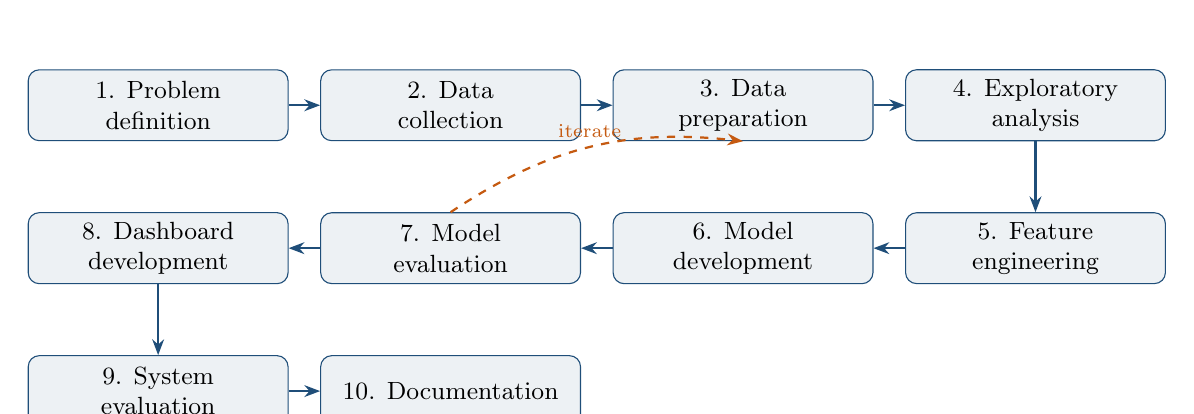
\begin{tikzpicture}[node distance=4mm and 4mm, every node/.style={font=\small},
  box/.style={draw=brand, rounded corners, fill=brand!8, minimum width=3.3cm, minimum height=9mm, align=center},
  arr/.style={-{Stealth[length=2mm]}, thick, brand}]
\node[box] (p1) {1. Problem\\definition};
\node[box, right=of p1] (p2) {2. Data\\collection};
\node[box, right=of p2] (p3) {3. Data\\preparation};
\node[box, right=of p3] (p4) {4. Exploratory\\analysis};
\node[box, below=9mm of p4] (p5) {5. Feature\\engineering};
\node[box, left=of p5] (p6) {6. Model\\development};
\node[box, left=of p6] (p7) {7. Model\\evaluation};
\node[box, left=of p7] (p8) {8. Dashboard\\development};
\node[box, below=9mm of p8] (p9) {9. System\\evaluation};
\node[box, right=of p9] (p10) {10. Documentation};
\draw[arr] (p1)--(p2); \draw[arr] (p2)--(p3); \draw[arr] (p3)--(p4); \draw[arr] (p4)--(p5);
\draw[arr] (p5)--(p6); \draw[arr] (p6)--(p7); \draw[arr] (p7)--(p8); \draw[arr] (p8)--(p9); \draw[arr] (p9)--(p10);
\draw[arr, dashed, accent] (p7.north) to[bend left=20] node[above, font=\scriptsize]{iterate} (p3.south);
\end{tikzpicture}
\caption{Project lifecycle, adapted from CRISP-DM}\label{fig:lifecycle}
\end{figure}

\section{Problem definition}
Four analytical problems were derived from the business questions:
\begin{enumerate}
  \item \textbf{Demand forecasting (regression).} Predict the number of units of each product sold in the
        next month. This supports production and inventory planning.
  \item \textbf{Large-order prediction (classification).} At the moment an order is entered, predict whether
        it will be large (\(\geq 10\) units). This supports allocation of stock and delivery capacity.
  \item \textbf{Segmentation (clustering).} Group products and market cells (region $\times$ channel $\times$
        customer type) with similar behaviour, to support portfolio and sales-force strategy.
  \item \textbf{Anomaly detection.} Detect unusual trading days and suspicious transactions. This supports
        monitoring and data-quality control.
\end{enumerate}

\section{Data}
The dataset comprises \NRows transactions with \NCols attributes, recorded between \DateMin and \DateMax. Each
record holds an identifier and date; the product (identifier, name, category, pack size, launch year); price
information (printed maximum retail price, list price, market price, discount percentage and unit selling
price); the quantity; the gross, discount and net sales values in Bangladeshi Taka (BDT); and the region,
channel and customer type. \Cref{tab:dictionary} in \cref{app:dictionary} gives the full data dictionary. The
data contain no personal identifiers.

\section{Evaluation design}
\subsection{Temporal hold-out}
Because the problems involve time, every supervised model is trained on the years \textbf{2020--2024} and
tested on \textbf{January 2025 -- September 2026}. This unseen period of \TestMonths months plays the role of
``the future''. Random train/test splits were deliberately not used, because they would let the models learn
from observations that come after the ones they predict \citep{bergmeir2012}.

\subsection{Hyper-parameter tuning}
Hyper-parameters were tuned only on the training years, using an \emph{expanding-window} validation. For
validation year $y \in \{2022, 2023, 2024\}$, the model is fitted on all months before $y$ and scored on $y$.
The configuration with the best mean validation score is then refitted on 2020--2024 and evaluated once on the
test period. For classification, the probability threshold was chosen in the same way: the model was fitted on
2020--2023 and the threshold that maximised F1 on 2024 was kept.

\subsection{Metrics}
For regression, the following measures were used, where $y_i$ is the actual and $\hat y_i$ the predicted value
for $n$ product-months:
\begin{align*}
\text{MAE} &= \tfrac{1}{n}\textstyle\sum_i |y_i-\hat y_i|, &
\text{RMSE} &= \sqrt{\tfrac{1}{n}\textstyle\sum_i (y_i-\hat y_i)^2}, &
R^2 &= 1-\frac{\sum_i (y_i-\hat y_i)^2}{\sum_i (y_i-\bar y)^2},\\
\text{MAPE} &= \tfrac{100}{n}\textstyle\sum_i \frac{|y_i-\hat y_i|}{\max(y_i,1)}, &
\text{WAPE} &= 100\,\frac{\sum_i |y_i-\hat y_i|}{\sum_i y_i}. &&
\end{align*}
WAPE is preferred for business communication because it weights each product by its volume. For
classification, accuracy, precision, recall, F1, ROC-AUC, PR-AUC and the lift in the top decile were reported.
For clustering, the silhouette coefficient, the Davies--Bouldin index and the Calinski--Harabasz index were
reported. Anomaly detectors were evaluated by precision and recall on a copy of the data containing planted
errors of known type.

\subsection{Benchmarks}
Following \citet{makridakis2018}, every forecasting model is compared with two naive rules: \emph{naive}
(next month = this month) and \emph{seasonal naive} (next month = the same month last year). At company level,
Holt--Winters and SARIMA serve as statistical benchmarks. The majority-class rule is the benchmark for
classification.

\section{Statistical analysis}
The exploratory phase used descriptive statistics, Spearman rank correlation (robust to the skewed
distributions found), Kruskal--Wallis tests for differences between groups, and chi-square tests of
independence. Because the sample is very large, almost any difference is statistically significant.
\emph{Effect sizes} ($\varepsilon^2$, $\rho^2$ and Cram\'er's $V$) were therefore reported and used to judge
practical importance. A fixed-effects log--log regression estimated the price elasticity of demand
\citep{wooldridge2020}.

\section{Two complementary modelling studies}
The predictive work was carried out twice, with different aims. The \emph{production study}
(\cref{ch:models}) builds the best possible models for the business: rich features, randomised hyper-parameter
search over expanding-window folds, statistical benchmarks and forecast reconciliation. The
\emph{algorithm-level study} (\cref{ch:algorithms}) examines each of the nine algorithms named in the proposal
separately, with a simpler shared feature set, a single 2024 validation year and one transparent script per
algorithm. Its aims are to explain how each algorithm learns and fails, and to check the production results
with an independent implementation.

\section{Tools and environment}
The framework was implemented in Python~3 with pandas and NumPy for data handling \citep{mckinney2022},
SciPy and statsmodels for statistics and time-series models, scikit-learn for machine learning
\citep{pedregosa2011}, XGBoost for gradient boosting \citep{chen2016}, Matplotlib and Plotly for
visualisation, SQLite for the dimensional data store, and Streamlit for the web dashboard. The code is
version-controlled with Git and published on GitHub. The dashboard is deployed on Streamlit Community Cloud and
the website on GitHub Pages. The report was typeset in \LaTeX. All random processes use a fixed seed (42), so every result can be reproduced exactly.

\section{Ethical considerations}
The dataset contains no names, contact details or other personally identifiable information. Customers are
described only by type (for example, \emph{Retailer}) and region. The data were used solely for academic
purposes, in line with the ethical principles stated in the proposal. Model limitations and uncertainties are
reported transparently (\cref{sec:limitations}), so that forecasts are not over-trusted in decision-making.

\chapter[System Design, Data and Preprocessing]{System Design, Data\\ and Preprocessing}\label{ch:system}

\section{Architecture of the framework}
The framework is organised in layers that mirror the workflow in the proposal (\cref{fig:architecture}). Each
layer is a Python module with a single responsibility. The modules communicate only through files with stable
formats (Parquet, SQLite and JSON), so any layer can be replaced without changing the others. For example, the
Streamlit dashboard could be swapped for Power BI reading the same SQLite store.

\begin{figure}[htbp]\centering
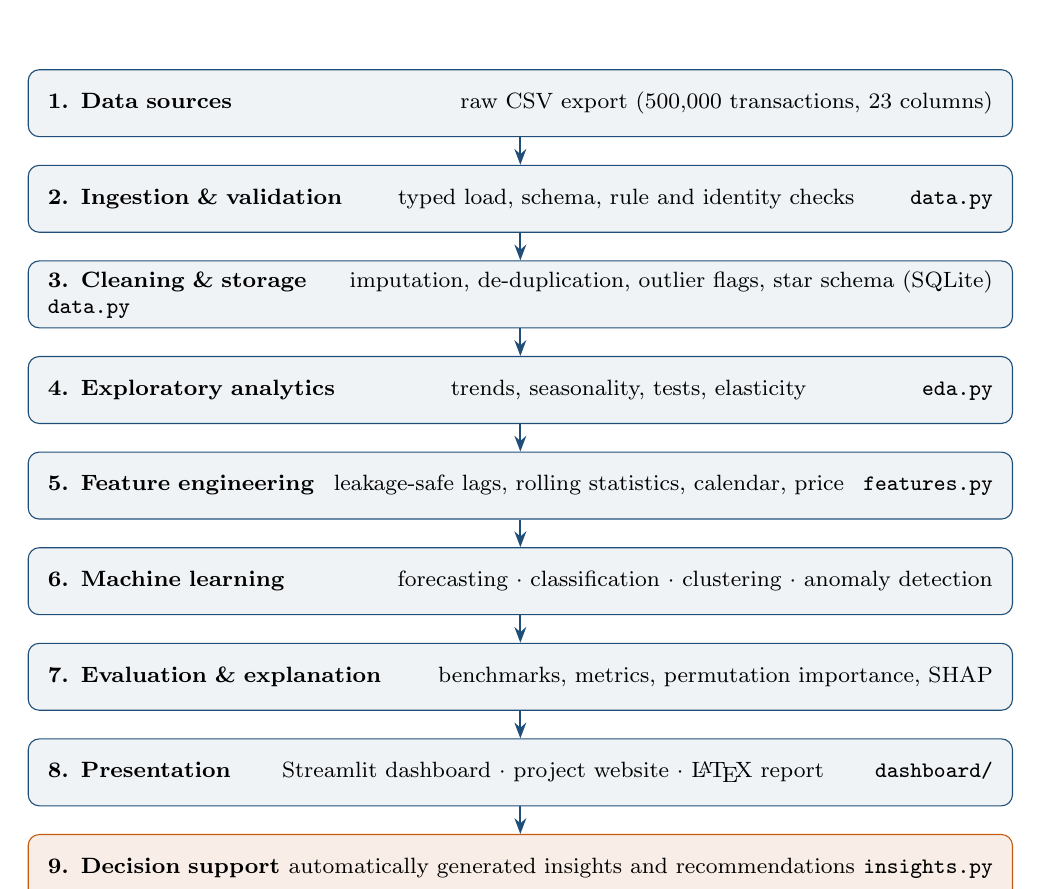
\begin{tikzpicture}[node distance=3.5mm, every node/.style={font=\footnotesize},
  L/.style={draw=brand, rounded corners, fill=brand!7, minimum width=12.5cm, minimum height=8.5mm, align=left, text width=12cm},
  arr/.style={-{Stealth[length=2mm]}, thick, brand}]
\node[L] (a) {\textbf{1. Data sources} \hfill raw CSV export (\NRows transactions, \NCols columns)};
\node[L, below=of a] (b) {\textbf{2. Ingestion \& validation} \hfill typed load, schema, rule and identity checks \hfill \texttt{data.py}};
\node[L, below=of b] (c) {\textbf{3. Cleaning \& storage} \hfill imputation, de-duplication, outlier flags, star schema (SQLite) \hfill \texttt{data.py}};
\node[L, below=of c] (d) {\textbf{4. Exploratory analytics} \hfill trends, seasonality, tests, elasticity \hfill \texttt{eda.py}};
\node[L, below=of d] (e) {\textbf{5. Feature engineering} \hfill leakage-safe lags, rolling statistics, calendar, price \hfill \texttt{features.py}};
\node[L, below=of e] (f) {\textbf{6. Machine learning} \hfill forecasting $\cdot$ classification $\cdot$ clustering $\cdot$ anomaly detection};
\node[L, below=of f] (g) {\textbf{7. Evaluation \& explanation} \hfill benchmarks, metrics, permutation importance, SHAP};
\node[L, below=of g] (h) {\textbf{8. Presentation} \hfill Streamlit dashboard $\cdot$ project website $\cdot$ \LaTeX{} report \hfill \texttt{dashboard/}};
\node[L, below=of h, fill=accent!10, draw=accent] (i) {\textbf{9. Decision support} \hfill automatically generated insights and recommendations \hfill \texttt{insights.py}};
\foreach \x/\y in {a/b,b/c,c/d,d/e,e/f,f/g,g/h,h/i} \draw[arr] (\x)--(\y);
\end{tikzpicture}
\caption{Layered architecture of the intelligent analytics framework}\label{fig:architecture}
\end{figure}

A single command, \texttt{python run\_pipeline.py}, executes all layers in order. It writes:
\begin{itemize}
  \item the cleaned dataset (\path{data/processed}) and the warehouse (\path{data/warehouse/dancake.db});
  \item metrics in JSON (\path{outputs/metrics}) and tables in CSV (\path{outputs/tables});
  \item every figure and \LaTeX{} table of this report (\path{report/figures}, \path{report/tables}), and a
        file of \LaTeX{} macros holding every number quoted in the text (\path{report/generated/numbers.tex});
  \item compact aggregated data for the dashboard and the website (\path{data/dashboard}).
\end{itemize}
Because no result is typed by hand, the report, dashboard and website cannot drift apart. A new month of data
can be incorporated by re-running one command.

\section{The dataset}
\Cref{tab:dqsummary} summarises the dataset and the results of the validation layer. Each transaction belongs to
one of \NProducts products in 13 categories. These are sold across \NRegions regions through \NChannels
channels (General Trade, Modern Trade, Distributor, E-commerce) to \NCustTypes customer types (Retailer, Super
Shop, Distributor, Corporate, Online Customer). Five products were launched after 2020: Lachcha Semai, two
breads, a croissant and a cappuccino muffin gift pack.

\begin{table}[htbp]\centering\small
\caption{Dataset profile and data-quality validation results}\label{tab:dqsummary}
\begin{tabular}{@{}lr@{}}
\toprule
\textbf{Check} & \textbf{Result} \\ \midrule
Rows $\times$ columns & \NRows $\times$ \NCols \\
Period covered & \DateMin -- \DateMax \\
Products / regions / channels / customer types & \NProducts / \NRegions / \NChannels / \NCustTypes \\
Missing cells (incl.\ hidden placeholders such as ``NA'', ``-'') & 0 \\
Exact duplicate rows / duplicate transaction IDs & 0 / 0 \\
Domain-rule violations (quantity, price, discount, value) & 0 \\
Gross $=$ quantity $\times$ market price (max.\ abs.\ error) & $<10^{-11}$ BDT \\
Net $=$ gross $-$ discount (max.\ abs.\ error) & $<10^{-11}$ BDT \\
Year/month columns consistent with date & 100\% \\
Product ID $\rightarrow$ one name, category, pack size & 100\% \\
Statistical quantity outliers (flagged, retained) & \NOutlierFlags (\OutlierPct\%) \\
Warehouse reconciliation (SQL total $-$ pandas total) & 0.00 BDT \\ \bottomrule
\end{tabular}
\end{table}

\section{Preprocessing pipeline}
The pipeline is written defensively. It must work correctly on dirty data, not only on the delivered file,
which proved to be exceptionally clean. Its behaviour on dirty data was verified in two ways. Six hands-on
practice scripts deliberately damaged copies of the data and measured how much was repaired. In addition, the
automated tests in \texttt{tests/} inject missing values, duplicates and impossible values and assert that the
pipeline repairs them (\cref{app:reproduce}). The steps are applied in a fixed order, because some steps depend
on others.

\subsection{Data type conversion and validation}
Dates are parsed with an explicit format (\texttt{dd-mm-yy}) and numeric columns are coerced. Values that fail
to parse become missing, so they are never silently misread. Text fields are trimmed of spaces. The validation
step then produces a machine-readable quality report (\texttt{outputs/metrics/data\_quality.json}). The report
checks for missing values, hidden placeholder strings, duplicate rows and keys, and domain-rule violations. It
also checks the accounting identities between columns and the consistency of calendar fields and product
attributes.

\subsection{Missing-value treatment}
A decision hierarchy was implemented, following \citet{garcia2015}:
\begin{enumerate}
  \item \emph{derive} the value exactly from other columns where an identity exists (for example,
        $\text{quantity} = \text{gross}/\text{market price}$, or year and month from the date);
  \item \emph{drop} the row if an essential identifier (transaction ID, date, product) is missing, because a
        guess would amount to fabrication;
  \item \emph{impute} numeric gaps with the median of the same product, which is robust to skew;
  \item \emph{impute} product attributes with the product's mode, and label missing market attributes
        explicitly as ``Unknown'' so that they remain visible.
\end{enumerate}
In practice tests with 3\% of cells removed at random, deriving values from accounting identities restored
quantities, prices and sales values exactly. Simple mean imputation, by contrast, introduced errors of several
units per order.

\subsection{Duplicate removal}
Exact duplicates are removed first. Duplicate keys, meaning the same transaction ID with differing values, are
resolved by keeping the most complete version. IDs are compared after upper-casing and trimming, so that hidden
duplicates such as `` dc2020000001'' are caught. Near-duplicates (same date, product, region, channel and
quantity but different IDs) are only \emph{flagged}. In sales data they are usually genuine repeat orders.

\subsection{Outlier detection and treatment}
Order quantities are strongly right-skewed (skewness \QtySkew; median \QtyMedian units). Each product also has
its own typical order size. A global $z$-score therefore flags too many small-product orders and too few
large-product ones. Four methods were compared in the practice phase: the IQR rule, the $z$-score, the MAD-based
modified $z$-score, and a per-product IQR rule on the log scale. The last of these was the most balanced, and
it is the method used in the pipeline:
\[
  \text{flag}_i = \bigl[\, \log(1+q_i) \notin [\,Q_1^{(p)} - 1.5\,\text{IQR}^{(p)},\; Q_3^{(p)} + 1.5\,\text{IQR}^{(p)}\,] \bigr],
\]
where the quartiles are computed separately for each product $p$. Impossible values (for example, a quantity
below one or a discount above 50\%) are treated as errors: they are blanked and re-derived. Unusual but possible
values are flagged and kept. The real data contained \NOutlierFlags such flags (\OutlierPct\% of orders), all
plausible bulk orders, and no impossible values.

\subsection{Normalisation and encoding}
Scaling is not applied globally. It is applied \emph{inside} each model's pipeline, fitted on the training rows
only, to avoid leakage. Count-like features are log-transformed, $\log(1+x)$, to stabilise variance, and they
are then standardised for scale-sensitive models (linear regression, KNN and SVR). Nominal categories (region,
channel, customer type, category) are one-hot encoded. Month is encoded cyclically as
$(\sin 2\pi m/12, \cos 2\pi m/12)$, so that December and January are neighbours. High-cardinality interactions
(channel $\times$ region, product) are target-encoded with additive smoothing,
\[
  \tilde\mu_k = \frac{n_k \bar y_k + m\,\bar y}{n_k + m}, \qquad m=50,
\]
using training data only. Rare levels are thereby shrunk towards the overall mean.

\subsection{Feature engineering for demand forecasting}
Transactions were aggregated into a \emph{panel} of \PanelSeries products $\times$ months. Each feature for
month $t$ uses only information available at the end of month $t-1$, or information that is planned in advance
(\cref{tab:features}). The same feature function is used for training, testing and future forecasting, so the
rule is enforced in one place. One instructive check compared a correct three-month rolling mean (shifted
before rolling) with a ``leaky'' version that included the current month. The leaky version correlated more
strongly with the target, which is exactly why leakage is tempting and dangerous \citep{kaufman2012}.

\begin{table}[htbp]\centering\small
\caption{Features of the demand-forecasting model (\PanelFeatures in total)}\label{tab:features}
\begin{tabularx}{\linewidth}{@{}lX@{}}
\toprule
\textbf{Group} & \textbf{Features} \\ \midrule
History (lags) & units in months $t-1, t-2, t-3, t-6, t-12$ \\
Rolling statistics & mean of the previous 3, 6 and 12 months; standard deviation of the previous 3 months \\
Momentum & last month's year-on-year growth; 12-month trend ratio \\
Price (planned) & list price of month $t$; year-on-year list-price change \\
Product & category (one-hot); pack weight in grams; gift-pack indicator; months since launch \\
Calendar & month number; cyclical month (sine, cosine); December and February indicators; days in month; time index \\ \bottomrule
\end{tabularx}
\end{table}

\section{Dimensional data store}
The cleaned data are loaded into a star schema in SQLite (\cref{fig:star}). The fact table \texttt{fact\_sales}
holds one row per transaction with its measures. The dimensions describe products, dates (including a
Friday--Saturday weekend flag, as in Bangladesh) and the 220 market segments formed by region, channel and
customer type. Indexes on the foreign keys make typical KPI queries return in well under a second. A
reconciliation check confirms that total net sales in the warehouse equal the total in the cleaned dataset to
the last paisa. \Cref{app:sql} lists example analytical SQL queries.

\begin{figure}[htbp]\centering
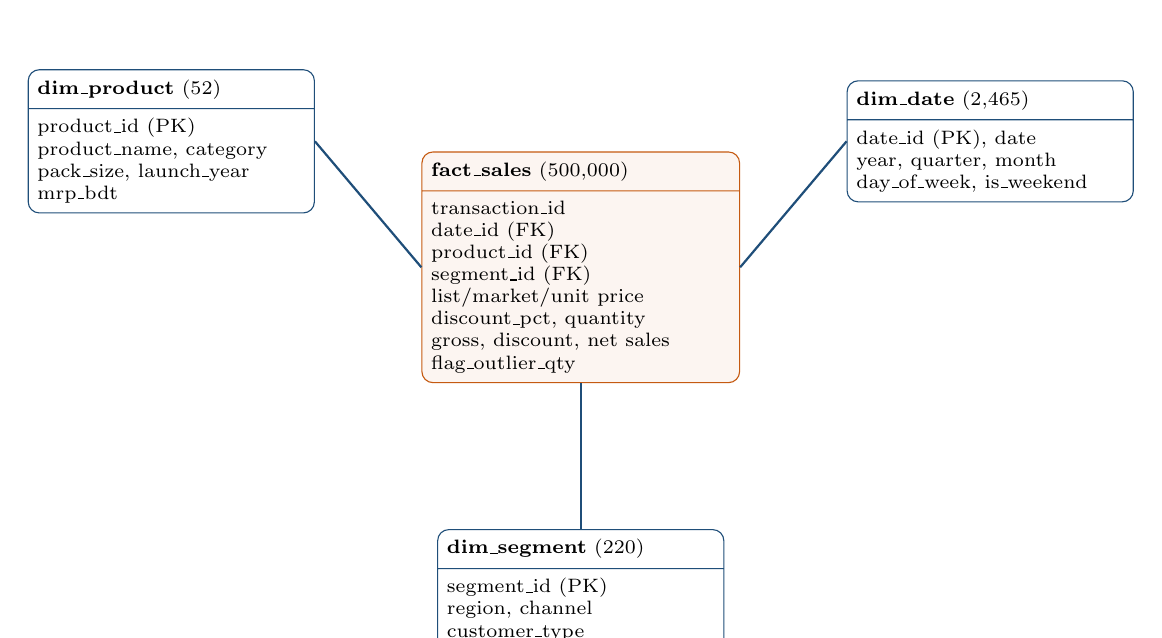
\begin{tikzpicture}[every node/.style={font=\scriptsize},
  T/.style={draw=brand, rectangle split, rectangle split parts=2, rounded corners, fill=white, text width=3.4cm, align=left},
  F/.style={T, draw=accent, fill=accent!6, text width=3.8cm}]
\node[F] (f) at (0,0) {\textbf{fact\_sales} (\NRows)\nodepart{second}transaction\_id\\date\_id (FK)\\product\_id (FK)\\segment\_id (FK)\\list/market/unit price\\discount\_pct, quantity\\gross, discount, net sales\\flag\_outlier\_qty};
\node[T] (p) at (-5.2,1.6) {\textbf{dim\_product} (\NProducts)\nodepart{second}product\_id (PK)\\product\_name, category\\pack\_size, launch\_year\\mrp\_bdt};
\node[T] (d) at (5.2,1.6) {\textbf{dim\_date} (2,465)\nodepart{second}date\_id (PK), date\\year, quarter, month\\day\_of\_week, is\_weekend};
\node[T] (s) at (0,-4.1) {\textbf{dim\_segment} (220)\nodepart{second}segment\_id (PK)\\region, channel\\customer\_type};
\draw[thick, brand] (f.west) -- (p.east); \draw[thick, brand] (f.east) -- (d.west); \draw[thick, brand] (f.south) -- (s.north);
\end{tikzpicture}
\caption{Star schema of the analytical data store}\label{fig:star}
\end{figure}

\chapter{Exploratory Data Analysis}\label{ch:eda}

This chapter answers the descriptive question, \emph{what happened?}, and begins to answer \emph{why}. All
results were computed on the full cleaned dataset by \texttt{eda.py}.

\section{Overall performance and growth}
Over the whole period, the company sold \TotalUnits million units in \NRows orders, worth \BDT\TotalSales
million in net sales. The average order was worth \BDT\AOV, and discounts averaged \AvgDiscount\% of gross
value, a cost of \BDT\DiscountCost million. \Cref{tab:annual} and \cref{fig:trend} show steady growth. Between
the first and the last complete year (2020--2025), net sales grew at a compound annual rate of \CAGRSales\%.
Sales in January--September 2026 were \YTDGrowth\% above the same months of 2025.

\begin{table}[htbp]
\centering
\small
\caption{Annual performance summary, 2020--2026}
\label{tab:annual}
\begin{adjustbox}{max width=\linewidth}
\begin{tabular}{lrrrrrrr}
\toprule
\textbf{Year} & \textbf{Orders} & \textbf{Units} & \textbf{Net sales (BDT M)} & \textbf{AOV (BDT)} & \textbf{Avg price} & \textbf{Disc. \%} & \textbf{YoY \%} \\
\midrule
2020 & 74,788 & 398,005 & 28.62 & 382.7 & 72.0 & 2.34 & -- \\
2021 & 73,636 & 418,104 & 37.02 & 502.7 & 88.6 & 2.35 & +29.3 \\
2022 & 73,898 & 440,150 & 41.00 & 554.8 & 93.4 & 2.34 & +10.8 \\
2023 & 73,598 & 460,465 & 46.17 & 627.3 & 100.5 & 2.36 & +12.6 \\
2024 & 74,282 & 486,293 & 53.03 & 713.9 & 109.8 & 2.35 & +14.9 \\
2025 & 74,442 & 507,262 & 61.78 & 829.9 & 122.3 & 2.35 & +16.5 \\
2026* & 55,356 & 381,678 & 50.75 & 916.8 & 133.8 & 2.34 & -- \\
\bottomrule
\end{tabular}
\end{adjustbox}
\par\smallskip\parbox{0.92\linewidth}{\footnotesize\emph{Note:} * 2026 covers January--September only, so growth is not computed for it. AOV = average order value; price = mean unit selling price.}
\end{table}

\begin{figure}[htbp]\centering
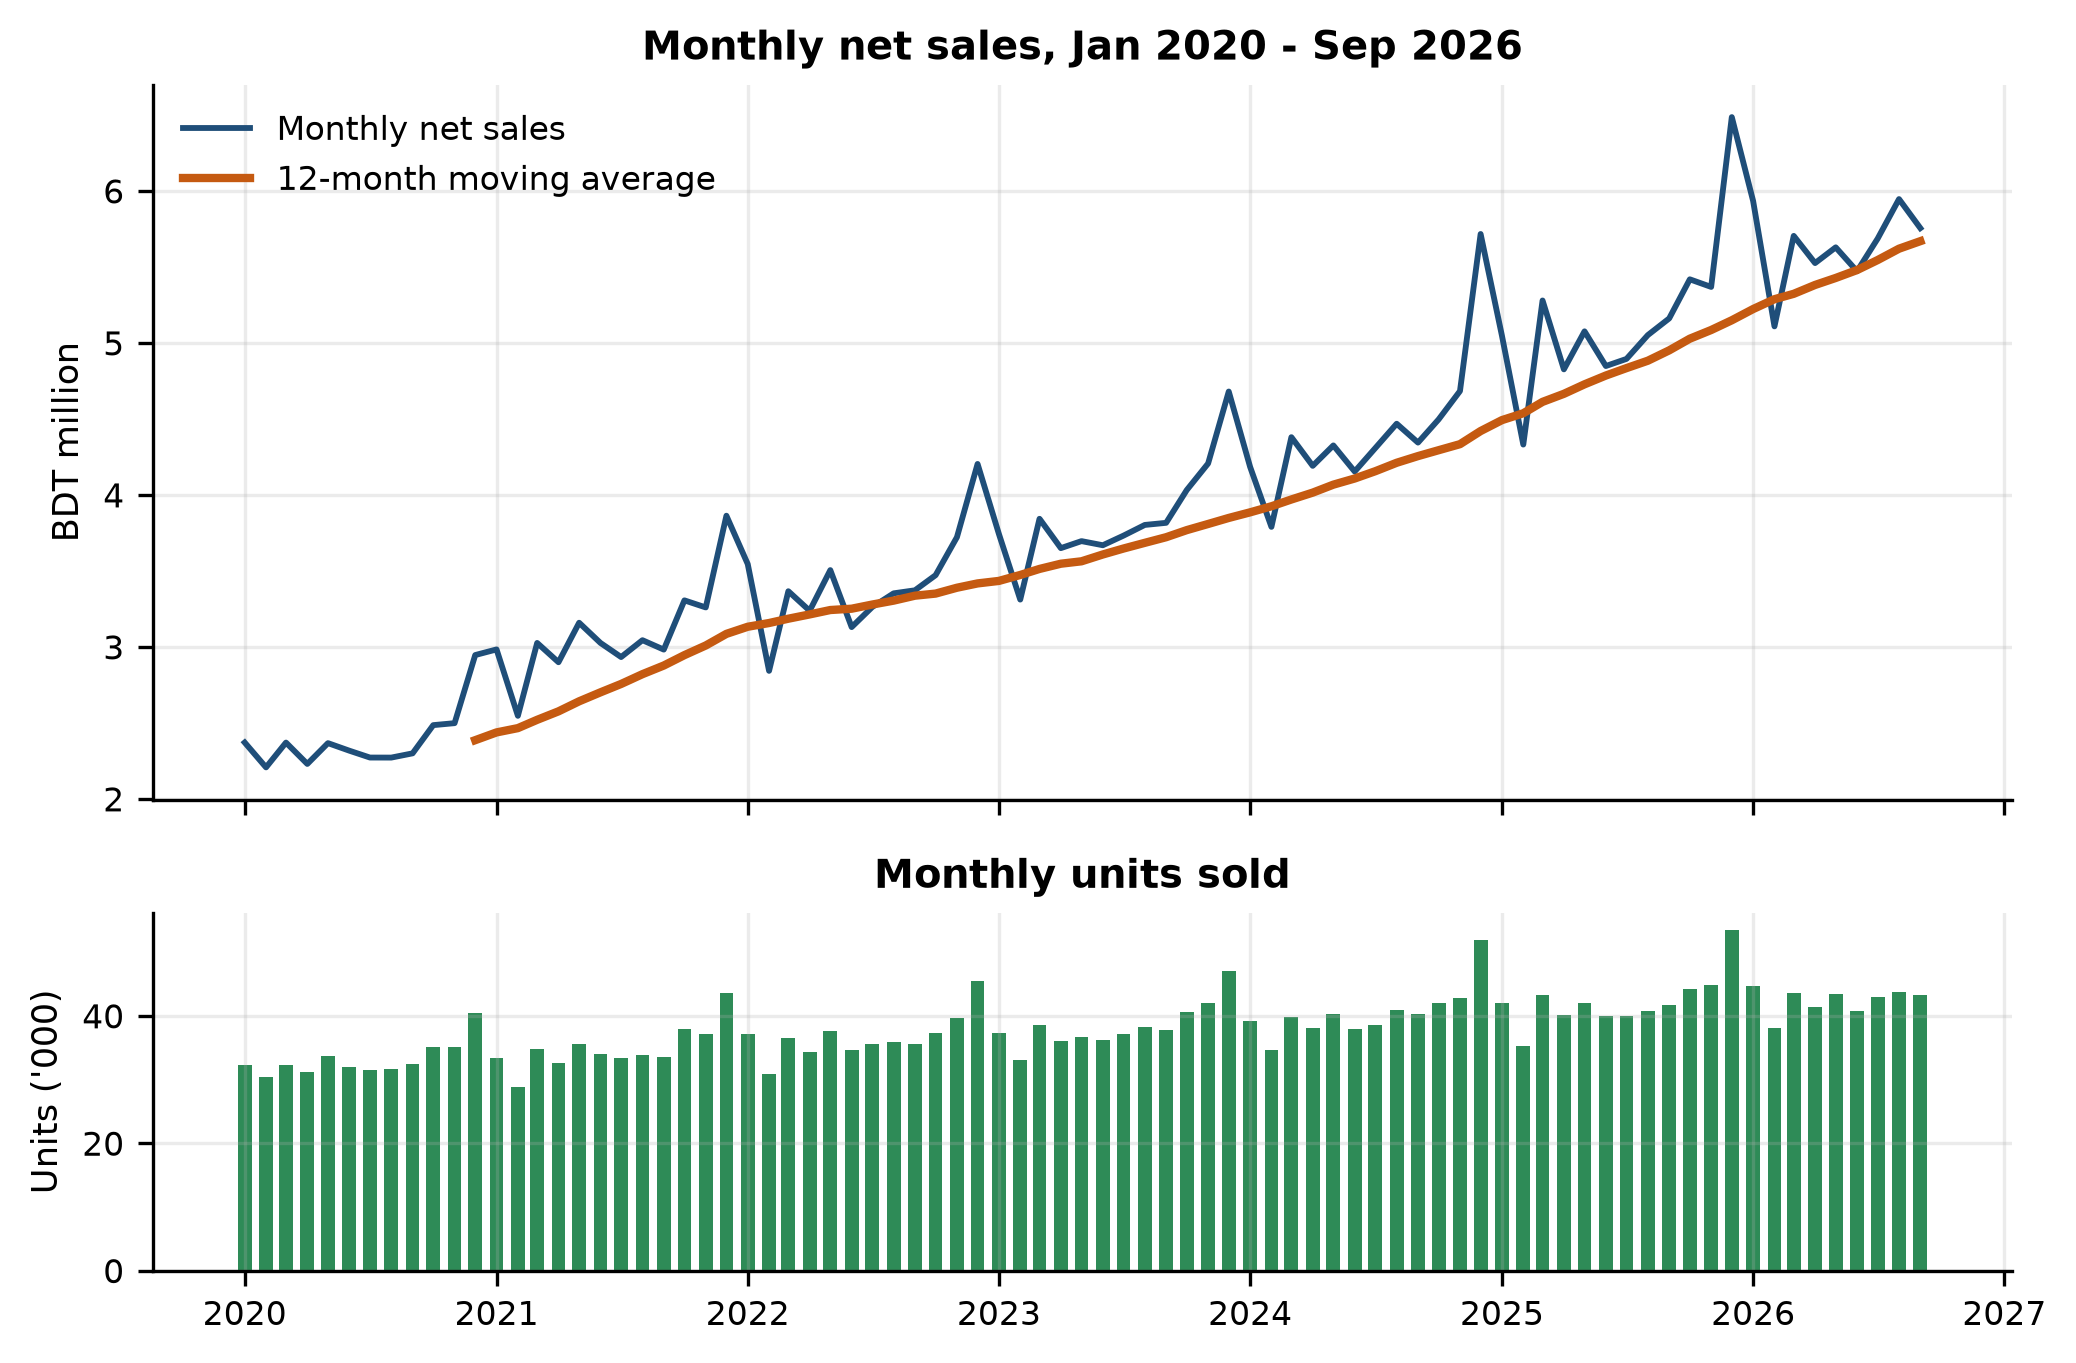
\includegraphics[width=\linewidth]{eda_monthly_trend}
\caption{Monthly net sales with 12-month moving average (top) and monthly units sold (bottom)}\label{fig:trend}
\end{figure}

\subsection{Where does growth come from?}
Units grew by only \CAGRUnits\% a year, whereas the average selling price grew by \CAGRPrice\% a year. Sales
growth can be decomposed exactly as $(1+g_{\text{sales}}) = (1+g_{\text{volume}})(1+g_{\text{price}})$.
\Cref{tab:pricevolume} and \cref{fig:pricevolume} show that, on average, about \AvgVolGrowth percentage points
of annual growth came from volume and \AvgPriceGrowth from price and product mix. The exceptional rise in 2021
coincides with the launch of higher-priced gift boxes, a mix effect. Later years reflect regular list-price
increases. This distinction matters for management: price-led growth cannot continue indefinitely without
eventually testing consumers' willingness to pay.

\begin{table}[htbp]
\centering
\small
\caption{Decomposition of annual sales growth into volume and price effects}
\label{tab:pricevolume}
\begin{adjustbox}{max width=\linewidth}
\begin{tabular}{lrrr}
\toprule
\textbf{Year} & \textbf{Sales growth \%} & \textbf{Volume growth \%} & \textbf{Avg price growth \%} \\
\midrule
2021 & +29.3 & +5.0 & +23.1 \\
2022 & +10.8 & +5.3 & +5.2 \\
2023 & +12.6 & +4.6 & +7.6 \\
2024 & +14.9 & +5.6 & +8.8 \\
2025 & +16.5 & +4.3 & +11.7 \\
\bottomrule
\end{tabular}
\end{adjustbox}
\par\smallskip\parbox{0.92\linewidth}{\footnotesize\emph{Note:} $(1+g_{sales}) = (1+g_{volume})(1+g_{price})$; price is net revenue per unit and therefore also reflects changes in product mix.}
\end{table}

\begin{figure}[htbp]\centering
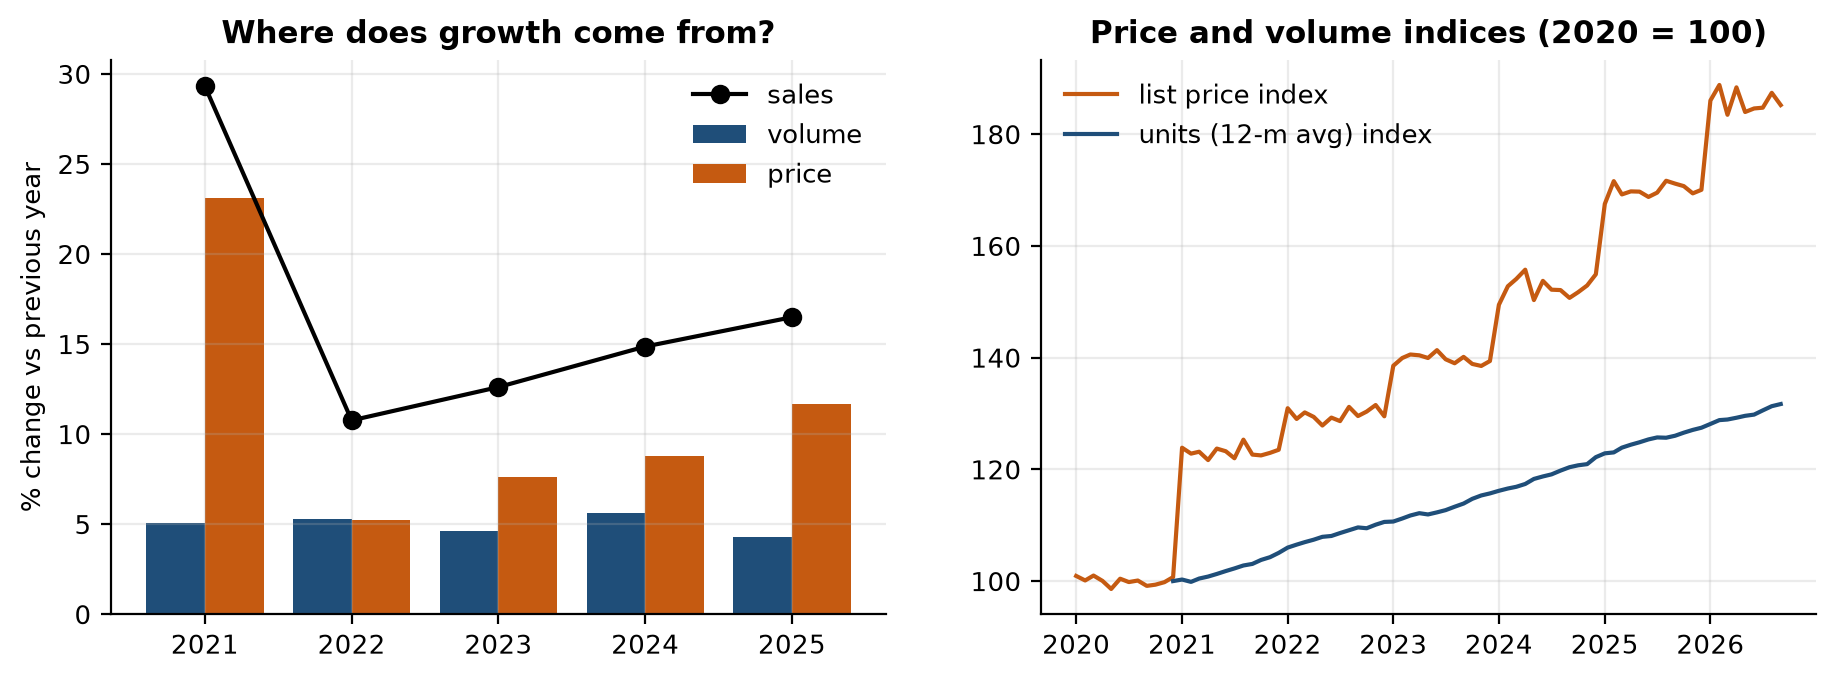
\includegraphics[width=\linewidth]{eda_price_volume}
\caption{Decomposition of growth (left) and price versus volume indices (right)}\label{fig:pricevolume}
\end{figure}

\subsection{Is demand sensitive to price?}
To separate the effect of price from that of general growth, the price elasticity of demand was estimated
with a fixed-effects regression on the product-month panel:
\[
  \log(\text{units}_{pt}) = \beta \log(\text{price}_{pt}) + \alpha_p + \gamma_{\text{year}(t)} + \delta_{\text{month}(t)} + \varepsilon_{pt}.
\]
The product effects $\alpha_p$ absorb differences in size between products. The year effects absorb common
market growth, and the month effects absorb seasonality. The estimated elasticity is
$\hat\beta = \Elasticity$, with a 95\% confidence interval from \ElasticityLo to \ElasticityHi (robust standard
errors; $p = \ElasticityP$; $R^2 = \ElasticityRtwo$). It is not significantly different from zero. Over the
observed range, demand therefore appears \emph{price-inelastic}. A naive regression without year effects gives
a misleading \emph{positive} elasticity of \ElasticityNaive, because prices and volumes both rose over time.
This is a textbook illustration of confounding, and the reason explanatory models need careful
specification \citep{shmueli2010}.

\section{Seasonality and calendar effects}
Sales show a clear annual cycle (\cref{fig:seasonality}). \PeakMonth is the strongest month, with a seasonal
index of \PeakIndex (average month = 100). October (\OctIndex) and November (\NovIndex) are also above average,
consistent with the year-end festive and gifting season. \TroughMonth is the weakest month (\TroughIndex). Part
of February's weakness is simply its shorter length: per trading day its index is \FebPerDay, while December's
per-day index remains high at \DecPerDay. A Kruskal--Wallis test on detrended daily sales confirms that
calendar month matters ($H = \KWMonthH$, $p<0.001$). By contrast, the day of the week has almost no effect: the
coefficient of variation of average daily sales across weekdays is only \DowCV\%.

\begin{figure}[htbp]\centering
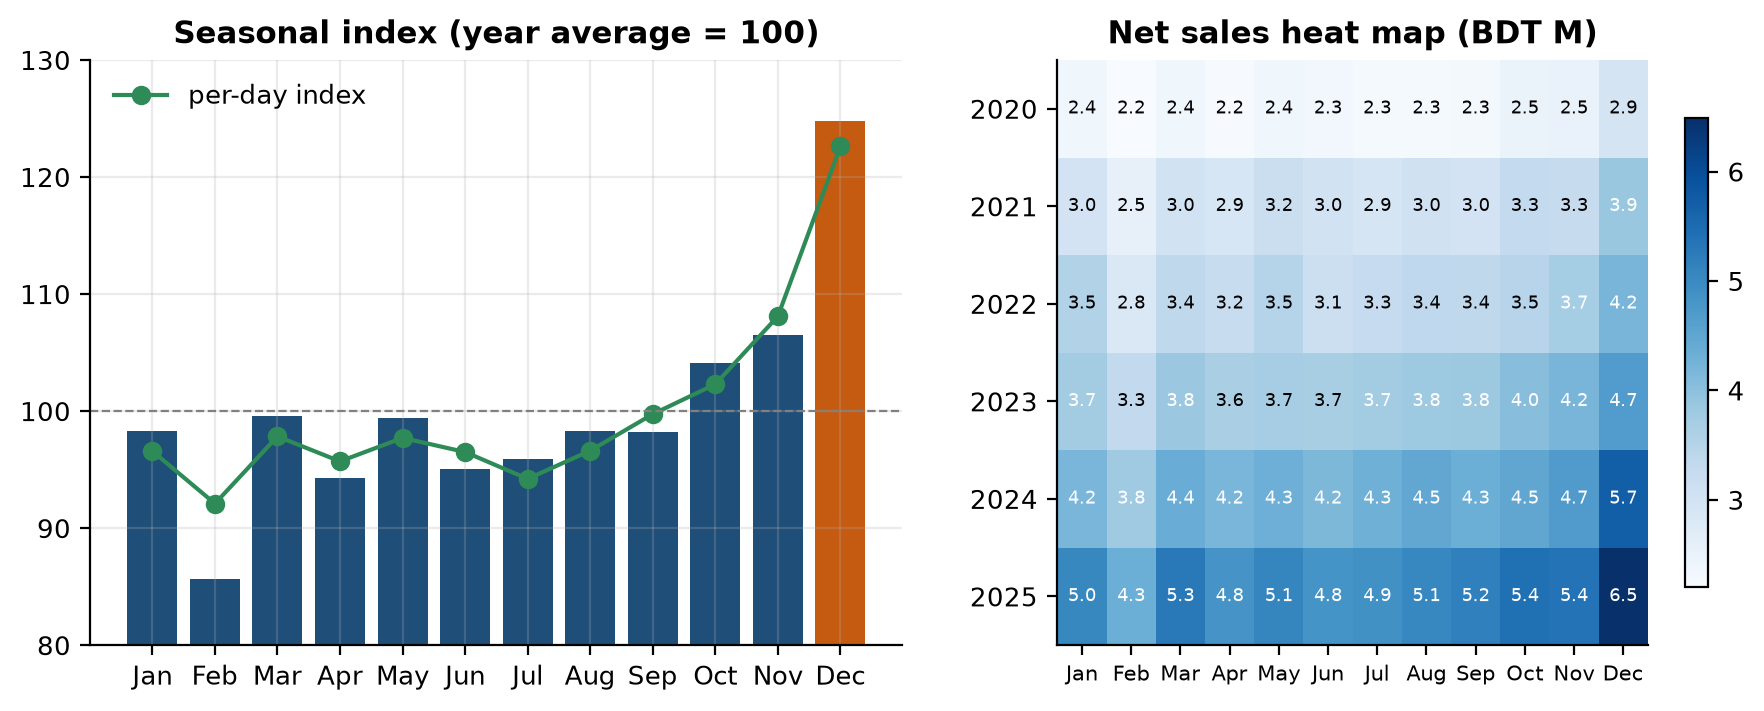
\includegraphics[width=\linewidth]{eda_seasonality}
\caption{Seasonal index by month (left) and year $\times$ month heat map of net sales (right)}\label{fig:seasonality}
\end{figure}

\section{Products and categories}
\Cref{tab:category} and \cref{fig:pareto} show the category structure. \TopCategory is the largest category
(\TopCategoryShare\% of sales), followed by Pound Cake and Swiss Roll. Layer Cake has the highest growth rate
(\FastCategoryCAGR\% a year). This growth comes mainly from gift-box variants added to the range in 2021, a
reminder that category growth figures combine organic growth with range changes. The Pareto analysis divides
the \NProducts products into \NClassA A-class products, which earn 80\% of revenue, and \NClassB B-class and
\NClassC C-class products. The ten best-selling products alone deliver \TopTenShare\% of net sales
(\cref{tab:topproducts}).

\begin{table}[htbp]
\centering
\small
\caption{Revenue and growth by product category}
\label{tab:category}
\begin{adjustbox}{max width=\linewidth}
\begin{tabular}{lrrrr}
\toprule
\textbf{Category} & \textbf{Net sales (BDT M)} & \textbf{Share \%} & \textbf{Products} & \textbf{CAGR 2020-25 \%} \\
\midrule
Muffin & 71.47 & 22.4 & 9 & +32.3 \\
Pound Cake & 61.76 & 19.4 & 12 & +9.7 \\
Swiss Roll & 38.81 & 12.2 & 4 & +9.6 \\
Fruit Cake & 28.90 & 9.1 & 5 & +9.9 \\
Layer Cake & 28.47 & 8.9 & 4 & +67.7 \\
Dry Cake & 25.59 & 8.0 & 3 & +9.4 \\
Cookie & 21.72 & 6.8 & 3 & +11.0 \\
Plain Cake & 16.57 & 5.2 & 6 & +10.4 \\
Velvet Cake & 11.75 & 3.7 & 1 & +10.3 \\
Classic Brownie & 6.27 & 2.0 & 1 & +10.8 \\
Premium & 4.02 & 1.3 & 1 & -- \\
Breakfast & 1.75 & 0.6 & 1 & -- \\
Bread & 1.28 & 0.4 & 2 & -- \\
\bottomrule
\end{tabular}
\end{adjustbox}
\par\smallskip\parbox{0.92\linewidth}{\footnotesize\emph{Note:} CAGR is computed between the first and last complete years. Categories launched after 2020 show growth from their launch year base.}
\end{table}
\begin{table}[htbp]
\centering
\small
\caption{Top ten products by net sales (Pareto/ABC analysis)}
\label{tab:topproducts}
\begin{adjustbox}{max width=\linewidth}
\begin{tabular}{lrrr}
\toprule
\textbf{Product} & \textbf{Net sales (BDT M)} & \textbf{Cumulative share \%} & \textbf{Class} \\
\midrule
MUF007 Cappuccino Muffin Gift Pack & 15.41 & 4.8 & A \\
MUF006 Vanilla Muffin Gift Box & 12.48 & 8.8 & A \\
LAY004 Vanilla Layer Cake Gift Box & 12.44 & 12.7 & A \\
LAY002 Chocolate Layer Cake Gift Box & 12.29 & 16.5 & A \\
MUF003 Chocolate Muffin Gift Box & 12.25 & 20.4 & A \\
MUF009 Chocochips Muffin & 11.99 & 24.1 & A \\
MUF008 Raisin Muffin & 11.80 & 27.8 & A \\
VEL001 Chocolate Velvet Cake & 11.75 & 31.5 & A \\
SWR002 Chocolate Swiss Roll & 11.68 & 35.2 & A \\
SWR004 Strawberry Swiss Roll & 10.44 & 38.5 & A \\
\bottomrule
\end{tabular}
\end{adjustbox}
\end{table}

\begin{figure}[htbp]\centering
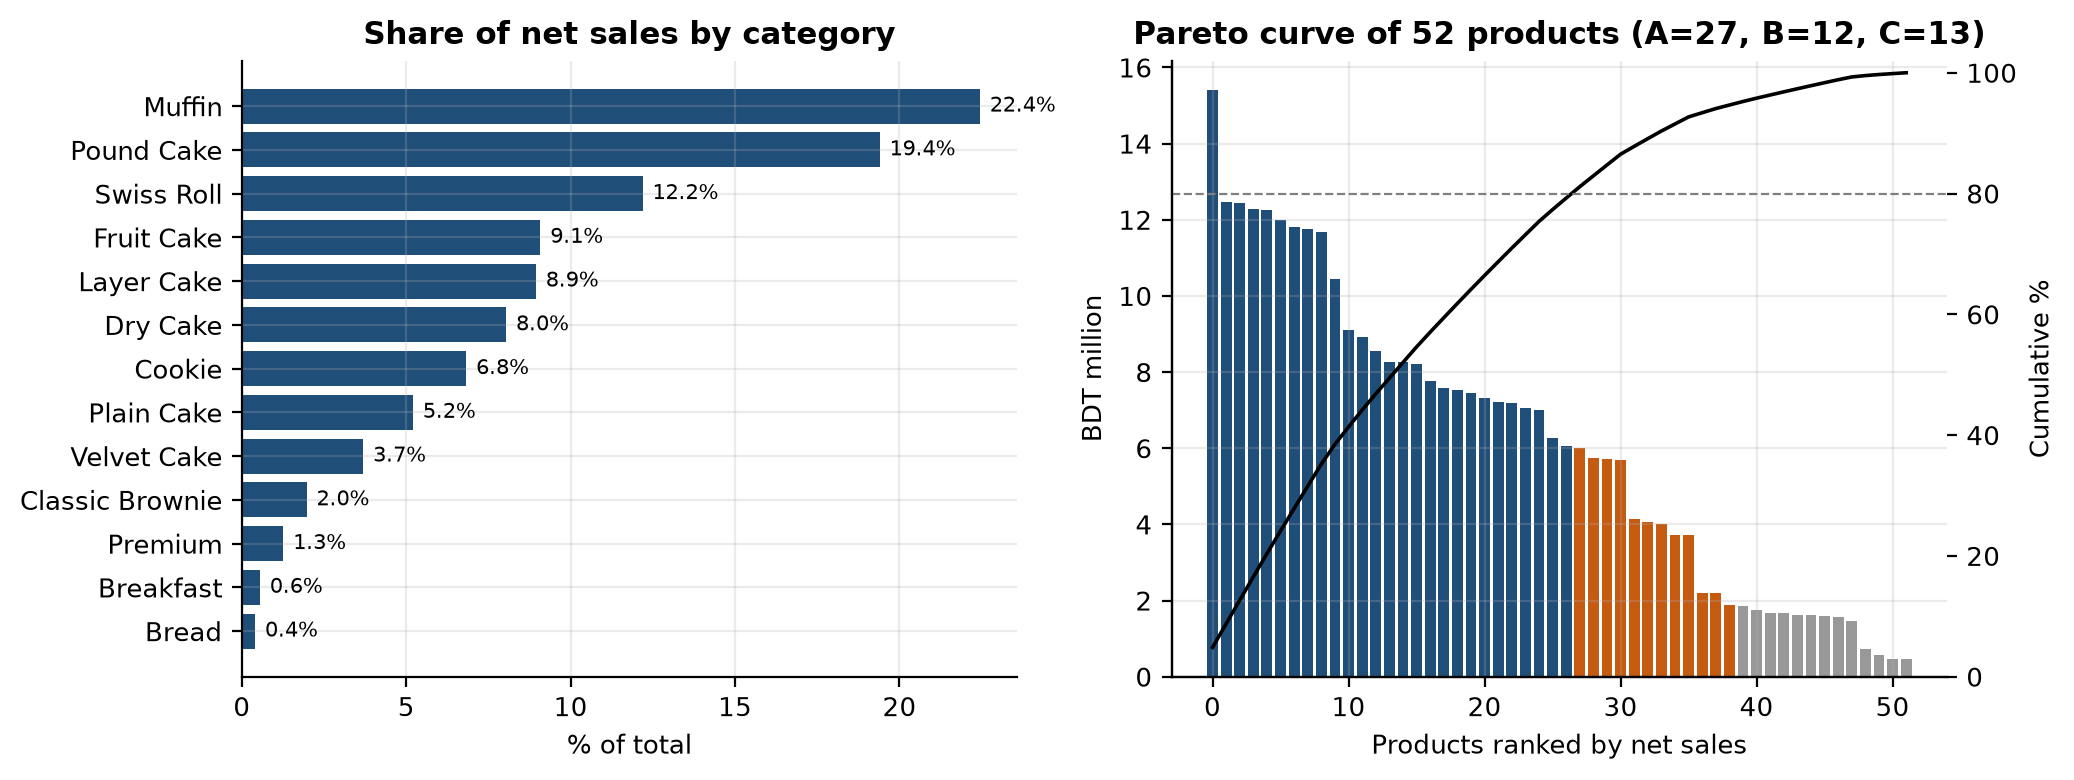
\includegraphics[width=\linewidth]{eda_category_pareto}
\caption{Share of net sales by category (left) and Pareto curve of products (right)}\label{fig:pareto}
\end{figure}

\section{Regions, channels and customers}
Sales are geographically concentrated. Dhaka generates \DhakaShare\% of net sales, and Dhaka and Chattogram
together \DhakaCtgShare\% (\cref{tab:segments}). General Trade is the main channel (\GTShare\%), followed by
Modern Trade (\MTShare\%), Distributors (\DistShare\%) and E-commerce (\EcomShare\%). The channels differ
sharply in order size. A distributor order averages \DistQty units, an E-commerce order \EcomQty, General Trade
\GTQty and Modern Trade \MTQty (\cref{fig:regionchannel}). Customer type, on the other hand, makes no difference
to order size (Kruskal--Wallis $p=\PCustType$), and average order values are almost identical across customer
types. Order size is therefore governed by the \emph{route to market}, not by who the customer is.

\begin{table}[htbp]
\centering
\footnotesize
\caption{Performance by region, channel and customer type}
\label{tab:segments}
\begin{adjustbox}{max width=\linewidth}
\begin{tabular}{llrrrrr}
\toprule
\textbf{Dimension} & \textbf{Level} & \textbf{Net sales (BDT M)} & \textbf{Share \%} & \textbf{Orders} & \textbf{AOV (BDT)} & \textbf{Units/order} \\
\midrule
Region & Dhaka & 139.76 & 43.9 & 169,661 & 823.8 & 7.85 \\
Region & Chattogram & 45.89 & 14.4 & 70,440 & 651.4 & 6.33 \\
Region & Gazipur & 25.74 & 8.1 & 39,853 & 645.9 & 6.34 \\
Region & Narayanganj & 21.23 & 6.7 & 35,195 & 603.1 & 5.93 \\
Region & Cumilla & 15.71 & 4.9 & 29,911 & 525.2 & 5.19 \\
Region & Sylhet & 15.27 & 4.8 & 29,901 & 510.6 & 4.92 \\
Region & Rangpur & 12.23 & 3.8 & 30,012 & 407.6 & 4.16 \\
Region & Rajshahi & 12.03 & 3.8 & 25,152 & 478.2 & 4.79 \\
Region & Khulna & 11.73 & 3.7 & 25,094 & 467.3 & 4.71 \\
Region & Mymensingh & 10.76 & 3.4 & 24,849 & 432.9 & 4.34 \\
Region & Barishal & 8.04 & 2.5 & 19,932 & 403.2 & 3.96 \\
Channel & General Trade & 145.21 & 45.6 & 260,431 & 557.6 & 5.32 \\
Channel & Modern Trade & 81.55 & 25.6 & 124,619 & 654.4 & 6.28 \\
Channel & Distributor & 72.90 & 22.9 & 64,861 & 1,123.9 & 11.43 \\
Channel & E-commerce & 18.72 & 5.9 & 50,089 & 373.7 & 3.66 \\
Customer type & Retailer & 143.28 & 45.0 & 224,582 & 638.0 & 6.19 \\
Customer type & Super Shop & 63.31 & 19.9 & 100,073 & 632.7 & 6.16 \\
Customer type & Distributor & 47.91 & 15.0 & 75,413 & 635.3 & 6.19 \\
Customer type & Online Customer & 31.95 & 10.0 & 49,759 & 642.0 & 6.17 \\
Customer type & Corporate & 31.93 & 10.0 & 50,173 & 636.4 & 6.21 \\
\bottomrule
\end{tabular}
\end{adjustbox}
\end{table}

\begin{figure}[htbp]\centering
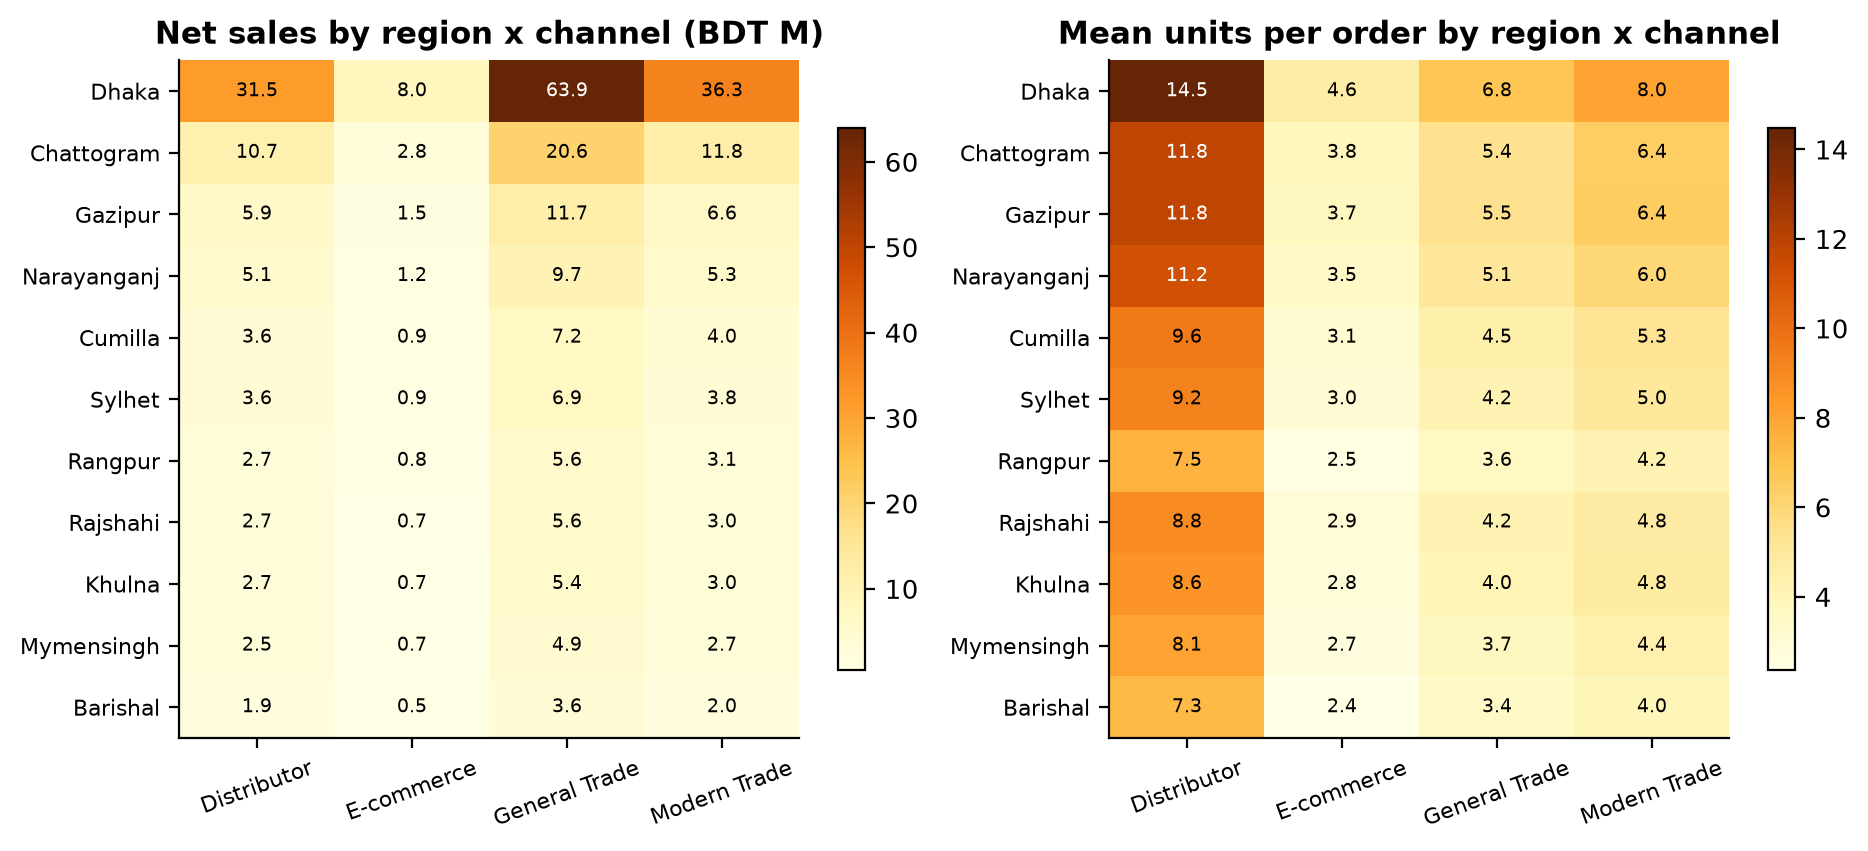
\includegraphics[width=\linewidth]{eda_region_channel}
\caption{Net sales (left) and mean units per order (right) by region and channel}\label{fig:regionchannel}
\end{figure}

\section{Distributions and relationships}
Order quantity and order value are strongly right-skewed, with skewness of \QtySkew and \ValueSkew
respectively (\cref{fig:distributions}). Most orders are small, and a long tail of bulk orders exists. These
shapes justify the use of medians, rank-based tests and log transformations throughout the analysis. The
Spearman correlation matrix (\cref{fig:correlation}) shows that order value is driven by both quantity
($\rho=\CorrSalesQty$) and price ($\rho=\CorrSalesPrice$). Quantity and price, however, are practically
unrelated ($\rho=\CorrQtyPrice$): customers do not buy fewer packs of the more expensive products.

\begin{figure}[htbp]\centering
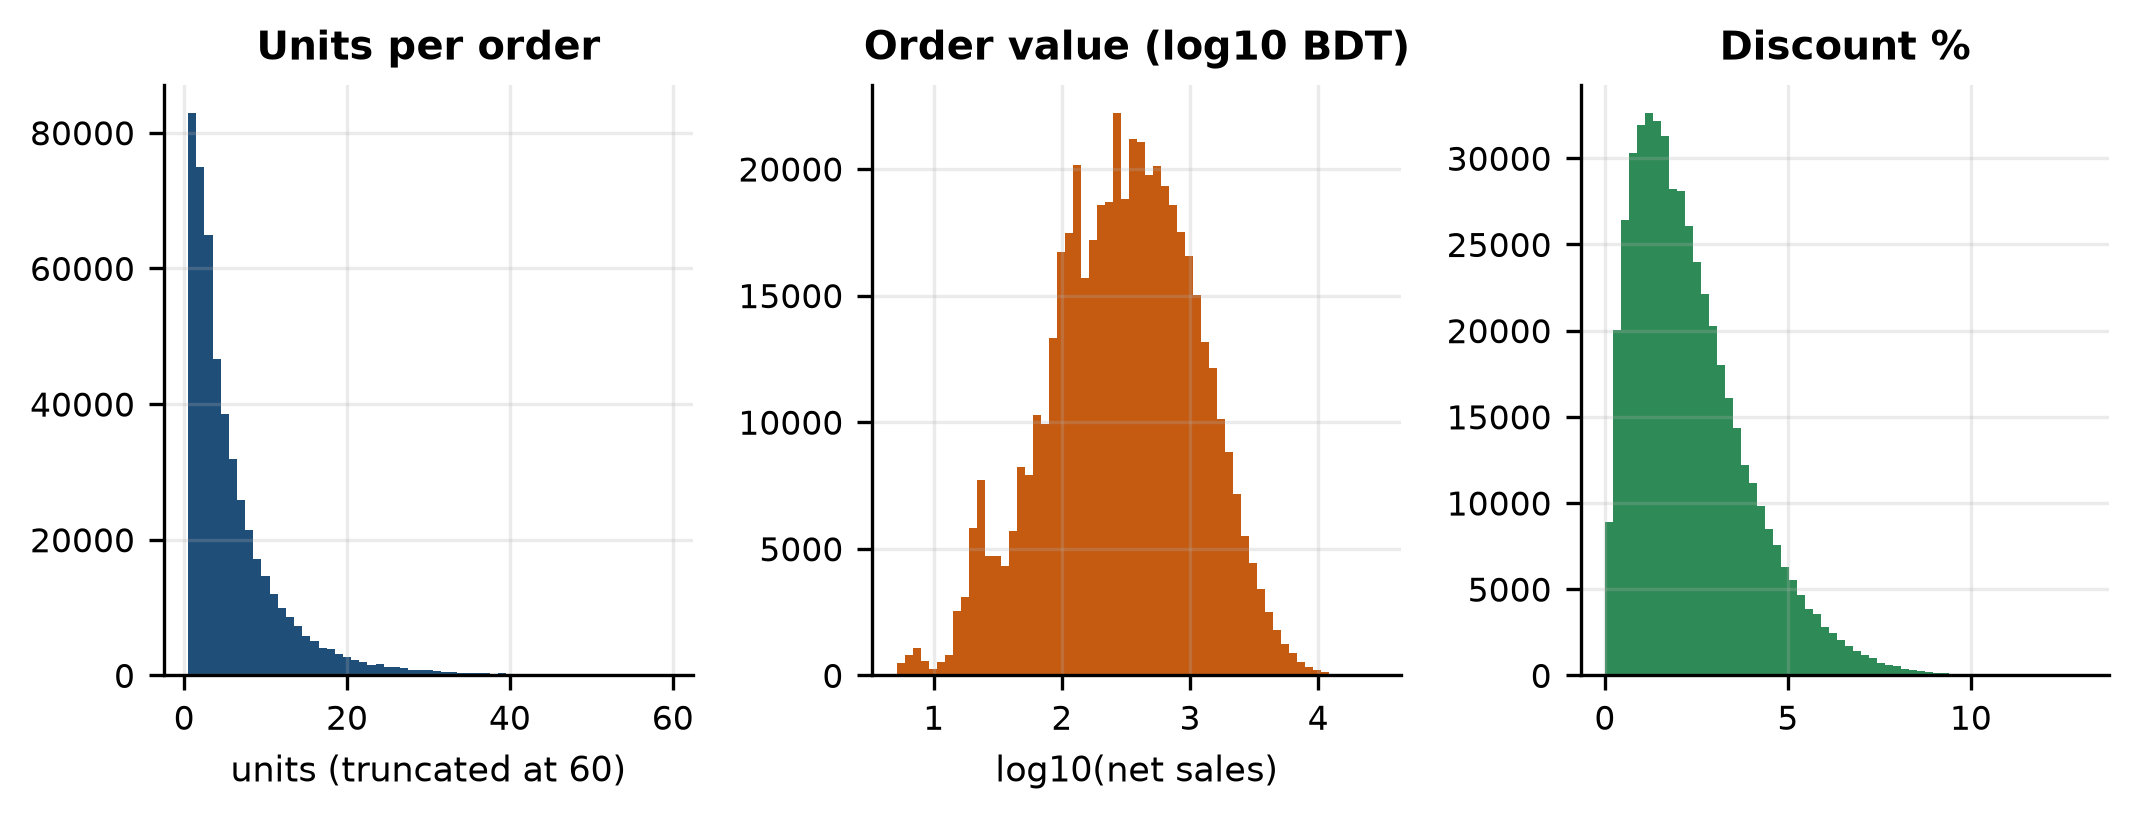
\includegraphics[width=\linewidth]{eda_distributions}
\caption{Distributions of units per order, order value (log scale) and discount}\label{fig:distributions}
\end{figure}

\begin{figure}[htbp]\centering
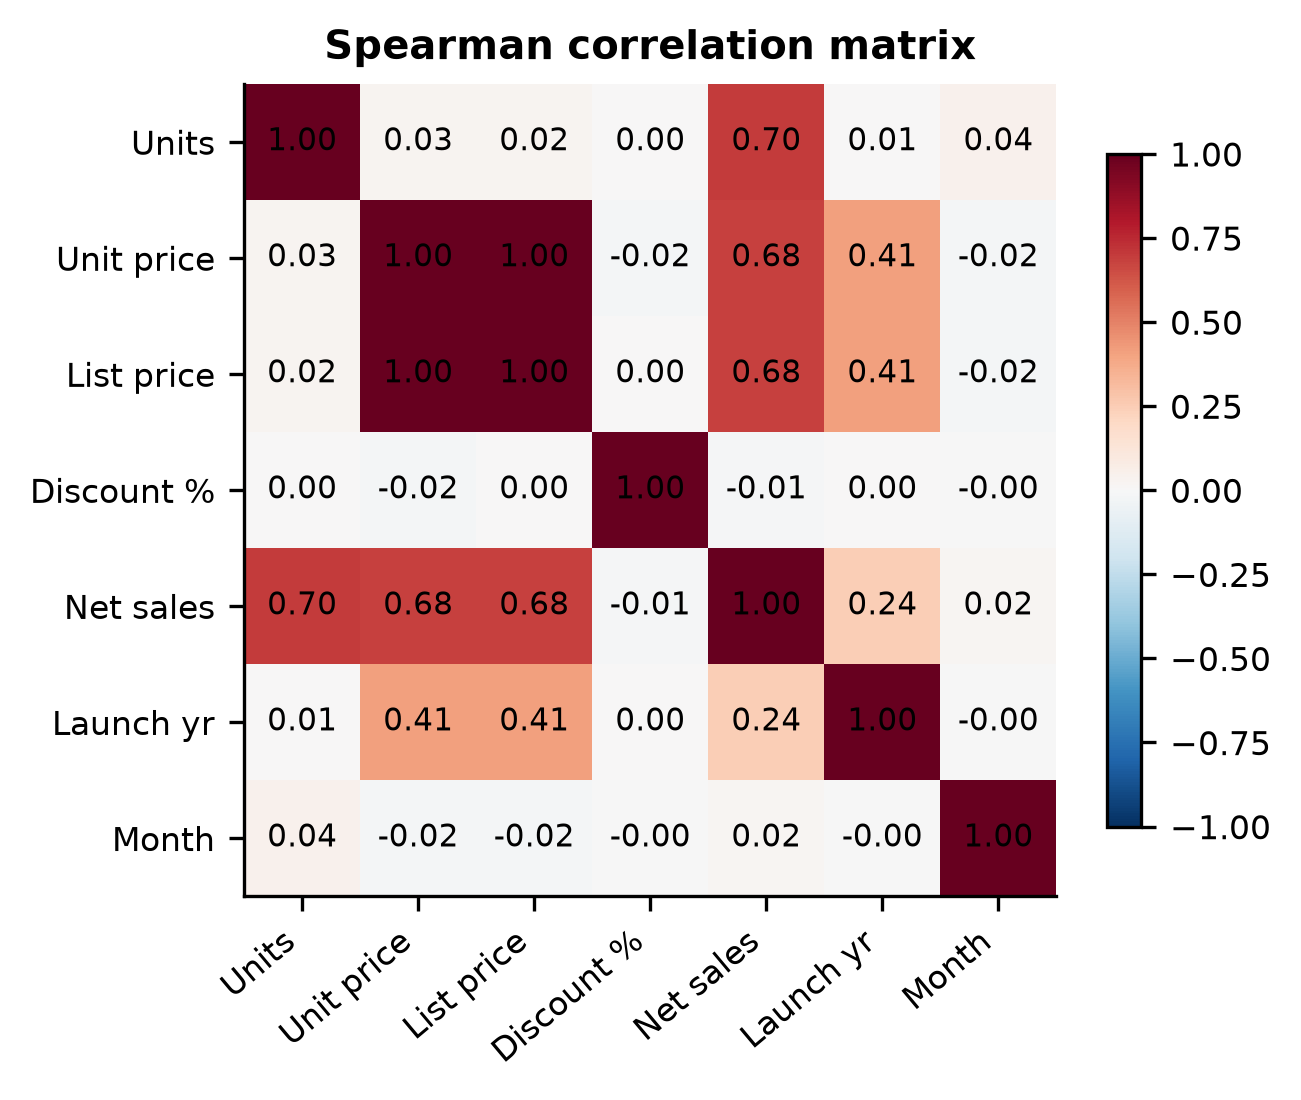
\includegraphics[width=.62\linewidth]{eda_correlation}
\caption{Spearman correlation matrix of the main numeric variables}\label{fig:correlation}
\end{figure}

\section{Hypothesis tests}
\Cref{tab:tests} formalises the main exploratory findings. With half a million observations, every difference
except two is statistically significant, so effect sizes are essential for interpretation. Channel explains the
most variation in order size ($\varepsilon^2=\EpsChannel$), followed by region ($\varepsilon^2=\EpsRegion$).
The association between channel and large orders is moderate (Cram\'er's $V=\CramerV$). Discount depth and
order size are \emph{uncorrelated} ($\rho=\RhoDisc$, $p=\PDisc$). The discounts given do not appear to
stimulate larger purchases. This is a potentially valuable finding, because discounts cost the company
\BDT\DiscountCost million over the period.

\begin{table}[htbp]
\centering
\small
\caption{Statistical tests of the main exploratory hypotheses}
\label{tab:tests}
\begin{adjustbox}{max width=\linewidth}
\begin{tabular}{llrrr}
\toprule
\textbf{Hypothesis (H0: no difference)} & \textbf{Test} & \textbf{Statistic} & \textbf{p-value} & \textbf{Effect size} \\
\midrule
Units/order by channel & Kruskal-Wallis & 43,269.88 & <0.001 & 0.0865 \\
Units/order by region & Kruskal-Wallis & 27,261.36 & <0.001 & 0.0545 \\
Units/order by customer type & Kruskal-Wallis & 2.62 & 0.623 & -0.0000 \\
Daily sales by month (detrended) & Kruskal-Wallis & 510.92 & <0.001 & 0.2293 \\
Discount \% vs units/order & Spearman rho & 0.00 & 0.479 & 0.0000 \\
Large order vs channel & Chi-square & 31,777.06 & <0.001 & 0.2521 \\
\bottomrule
\end{tabular}
\end{adjustbox}
\par\smallskip\parbox{0.92\linewidth}{\footnotesize\emph{Note:} Effect sizes: $\varepsilon^2$ for Kruskal--Wallis, $\rho^2$ for Spearman and Cram\'er's $V$ for chi-square. With $n=500{,}000$ almost any difference is `significant', so the effect size decides practical importance.}
\end{table}

\section{Summary of exploratory findings}
\begin{enumerate}
  \item Revenue growth is strong (\CAGRSales\% a year) but mostly price- and mix-driven; volume grows at \CAGRUnits\%.
  \item Demand is price-inelastic in the observed range, and discounts show no measurable effect on order size.
  \item Seasonality is pronounced, with a \PeakMonth peak and a \TroughMonth trough; weekdays do not matter.
  \item Revenue is concentrated: Dhaka provides \DhakaShare\% of sales and ten products provide \TopTenShare\%.
  \item Order size depends on channel and region, not on customer type.
\end{enumerate}
These findings informed the modelling choices in the next chapter. Seasonality and history features are used
for forecasting, channel and region for classification, and price, growth and seasonality for segmentation.

\chapter{Predictive Modelling and Evaluation}\label{ch:models}

This chapter answers the predictive question, \emph{what is likely to happen next?} It covers the four
analytical problems in turn: demand forecasting, large-order classification, segmentation and anomaly detection.

\section{Monthly demand forecasting}
\subsection{Set-up}
The forecasting panel contains \PanelSeries products observed monthly. There are \PanelTrain training rows
(2020--2024) and \PanelTest test rows (January 2025 -- September 2026). Each model predicts
$\log(1+\text{units})$, and the prediction is converted back to units. The log scale suits the multiplicative
nature of demand and stops the largest products from dominating the fit. Seven algorithms were tuned by
randomised search over the expanding-window folds described in \cref{ch:method}. \Cref{tab:hyper} in
\cref{app:hyper} lists the selected hyper-parameters.

\subsection{One-step-ahead results}
\Cref{tab:forecast} reports test performance when each month is forecast with the actual history up to the
previous month. This is the operational scenario of a monthly planning cycle. Every machine-learning model
clearly beats both naive baselines. The best model, \BestReg, reaches RMSE \BestRegRMSE units, WAPE
\BestRegWAPE\% and $R^2=\BestRegRtwo$. That is an RMSE \GainVsSNaive\% lower than the seasonal-naive rule
(\SNaiveRMSE) and \GainVsNaive\% lower than the naive rule (\NaiveRMSE).

\begin{table}[htbp]
\centering
\footnotesize
\caption{Monthly product-demand forecasting: test-set performance (one-step-ahead, Jan 2025--Sep 2026)}
\label{tab:forecast}
\begin{adjustbox}{max width=\linewidth}
\begin{tabular}{lrrrrrrrr}
\toprule
\textbf{Model} & \textbf{MAE} & \textbf{MSE} & \textbf{RMSE} & \textbf{R$^2$} & \textbf{MAPE \%} & \textbf{WAPE \%} & \textbf{CV RMSE} & \textbf{Fit (s)} \\
\midrule
Seasonal naive (same month last year) & 120.0 & 23,233 & 152.4 & 0.551 & 15.38 & 14.74 & -- & 0.0 \\
Naive (last month) & 139.8 & 31,051 & 176.2 & 0.400 & 18.00 & 17.17 & -- & 0.0 \\
Support Vector Regression & 90.6 & 13,271 & 115.2 & 0.744 & 12.26 & 11.13 & 0.2151 & 24.9 \\
Linear Regression & 91.3 & 13,861 & 117.7 & 0.732 & 11.48 & 11.21 & 0.1691 & 0.2 \\
XGBoost & 93.3 & 14,294 & 119.6 & 0.724 & 12.28 & 11.46 & 0.1917 & 94.8 \\
Random Forest & 93.0 & 14,413 & 120.1 & 0.722 & 12.04 & 11.42 & 0.1918 & 142.6 \\
Gradient Boosting & 95.7 & 15,113 & 122.9 & 0.708 & 12.51 & 11.76 & 0.1889 & 124.9 \\
K-Nearest Neighbors & 97.0 & 15,865 & 126.0 & 0.694 & 12.01 & 11.91 & 0.1951 & 6.8 \\
Decision Tree & 103.6 & 17,978 & 134.1 & 0.653 & 13.70 & 12.73 & 0.2077 & 8.1 \\
\bottomrule
\end{tabular}
\end{adjustbox}
\par\smallskip\parbox{0.92\linewidth}{\footnotesize\emph{Note:} Errors in units per product-month. CV RMSE is the mean validation RMSE on the log scale over the expanding-window folds 2022, 2023 and 2024 used for tuning. Baselines need no fitting.}
\end{table}

Three further observations stand out. First, the differences between the better models are small. RMSE values
range only from \BestRegRMSE to \WorstRegRMSE units, and linear regression on log features (\LinRMSE) is
competitive with the tree ensembles (random forest \RFRMSE, XGBoost \XGBRMSE). Once good lag and seasonal
features exist, the problem is largely log-linear, and model complexity adds little. This agrees with
\citet{makridakis2018}. Second, the single decision tree is the weakest learner (\DTRMSE), as expected from its
high variance; averaging many trees in a forest removes most of this weakness \citep{breiman2001}. Third, the
cross-validated scores on the training years rank the models similarly to the test scores. The validation
design therefore gives a reliable guide to future performance. \Cref{fig:forecastcomp} compares the models and
shows that predictions of \BestReg track the actual values closely across products of very different size.

\begin{figure}[htbp]\centering
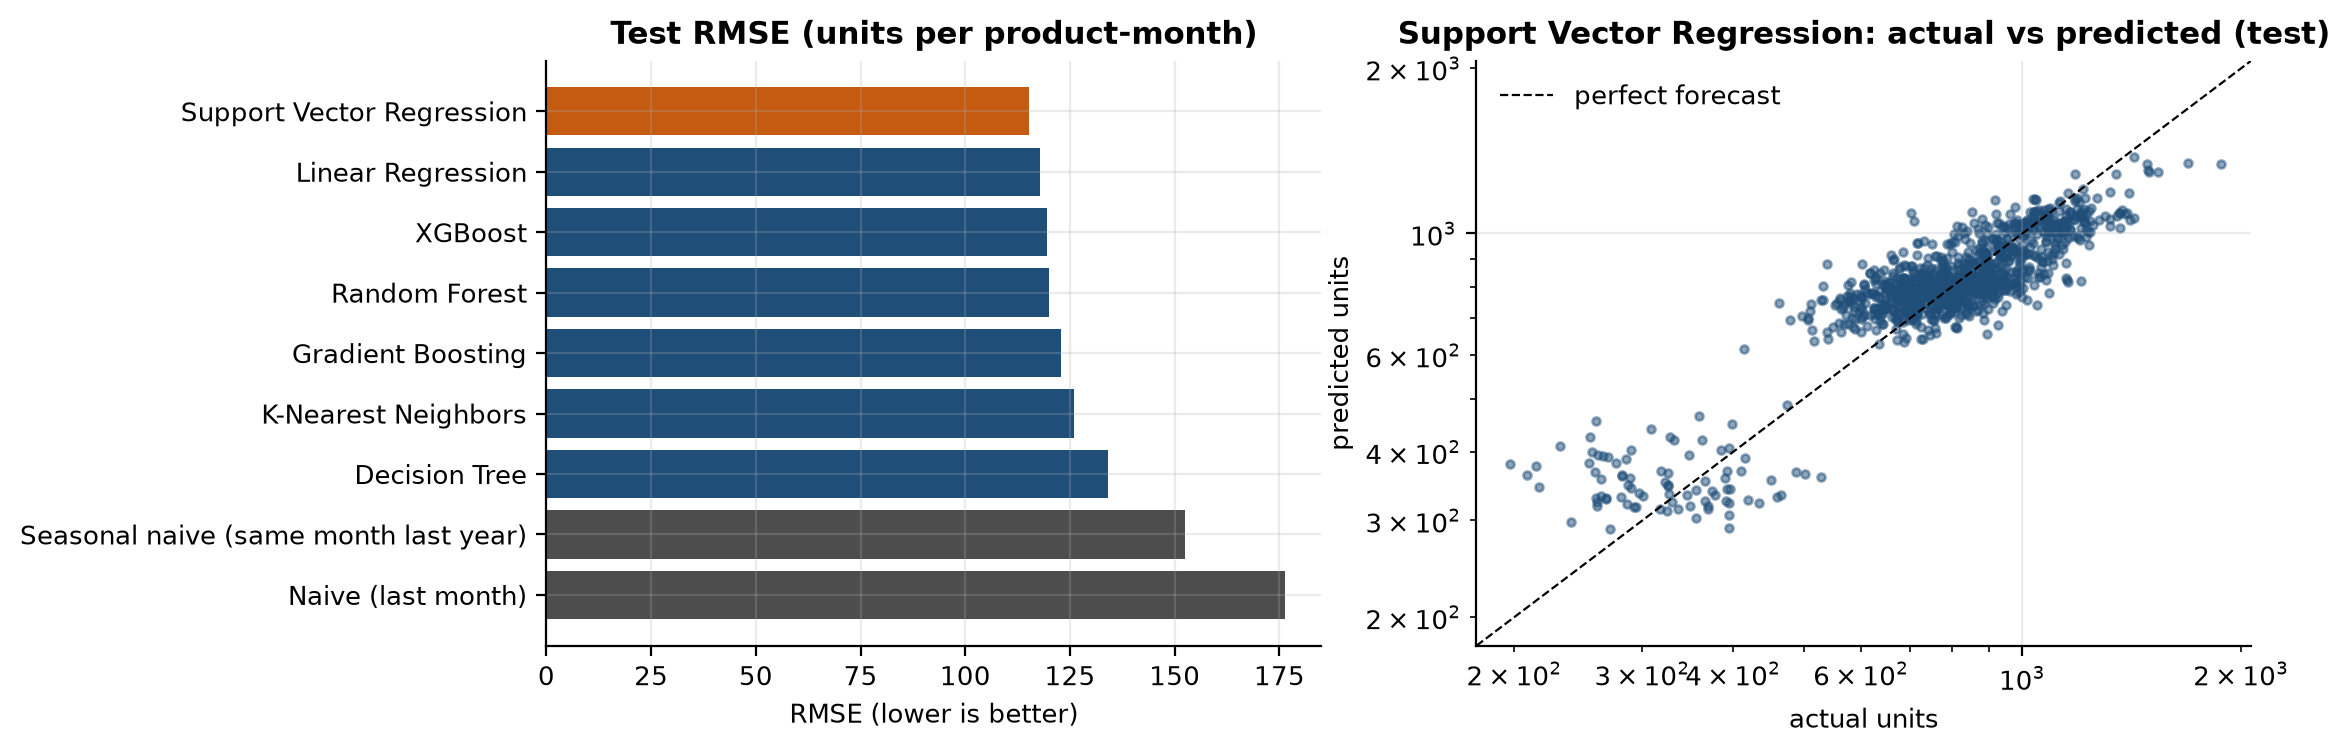
\includegraphics[width=\linewidth]{ml_forecast_comparison}
\caption{Test RMSE of all forecasting models (left; best model highlighted, baselines in grey) and actual versus predicted units for the best model (right)}\label{fig:forecastcomp}
\end{figure}

\subsection{Recursive multi-step results}
A harder test is to forecast all 21 test months from December 2024 \emph{without} seeing any actual data after
training. Each month's predictions are fed back in as history for the next month. This is the scenario of an
annual budget. \Cref{tab:recursive} shows that the best models degrade only modestly. \BestRec achieves a
WAPE of \BestRecWAPE\% ($R^2=\BestRecRtwo$), still far better than repeating the 2024 pattern. XGBoost degrades
the most under recursion. Errors compound when a model's own predictions become inputs, and boosted trees, which
fit the training data closely, are more exposed to this.

\begin{table}[htbp]
\centering
\small
\caption{Recursive 21-month forecast from December 2024 (no actual data used after training)}
\label{tab:recursive}
\begin{adjustbox}{max width=\linewidth}
\begin{tabular}{lrrrrr}
\toprule
\textbf{Model} & \textbf{MAE} & \textbf{RMSE} & \textbf{R$^2$} & \textbf{MAPE \%} & \textbf{WAPE \%} \\
\midrule
Random Forest & 91.0 & 117.0 & 0.736 & 11.85 & 11.18 \\
Support Vector Regression & 92.3 & 117.2 & 0.735 & 12.65 & 11.34 \\
Linear Regression & 94.1 & 121.4 & 0.715 & 11.73 & 11.56 \\
XGBoost & 104.1 & 137.5 & 0.635 & 16.17 & 12.79 \\
Seasonal naive (2024 pattern repeated) & 125.9 & 158.1 & 0.517 & 15.87 & 15.47 \\
\bottomrule
\end{tabular}
\end{adjustbox}
\end{table}

\subsection{Company-level forecasting and model reconciliation}
Product forecasts can be summed to a company total and compared with statistical models fitted directly to the
total series (\cref{tab:company}, \cref{fig:companyfc}). At this aggregate level, the Holt--Winters model with
additive trend and multiplicative seasonality is the most accurate, with a MAPE of only \HWMAPE\%. The summed
machine-learning forecasts are also accurate but slightly less so. The result is consistent with the literature:
smooth aggregate series favour statistical models, while the cross-learning ability of machine learning pays
off at the level of individual products. The framework therefore combines the two through \emph{top-down
reconciliation} \citep{athanasopoulos2009}. Holt--Winters sets the company total and its prediction interval,
and the machine-learning model distributes that total across products. Product plans then add up exactly to the
company plan.

\begin{table}[htbp]
\centering
\small
\caption{Company-level monthly units forecast, test period Jan 2025--Sep 2026}
\label{tab:company}
\begin{adjustbox}{max width=\linewidth}
\begin{tabular}{lrrr}
\toprule
\textbf{Model (company-total monthly units)} & \textbf{MAE} & \textbf{RMSE} & \textbf{MAPE \%} \\
\midrule
Holt-Winters (additive trend, multiplicative season) & 559 & 698 & 1.32 \\
SARIMA(1,1,1)(0,1,1)$_{12}$ on log units & 687 & 806 & 1.65 \\
Support Vector Regression one-step, summed over products & 712 & 875 & 1.68 \\
Random Forest recursive, summed over products & 1,186 & 1,386 & 2.77 \\
Seasonal naive (2024 repeated) & 2,549 & 2,817 & 6.00 \\
\bottomrule
\end{tabular}
\end{adjustbox}
\end{table}

\begin{figure}[htbp]\centering
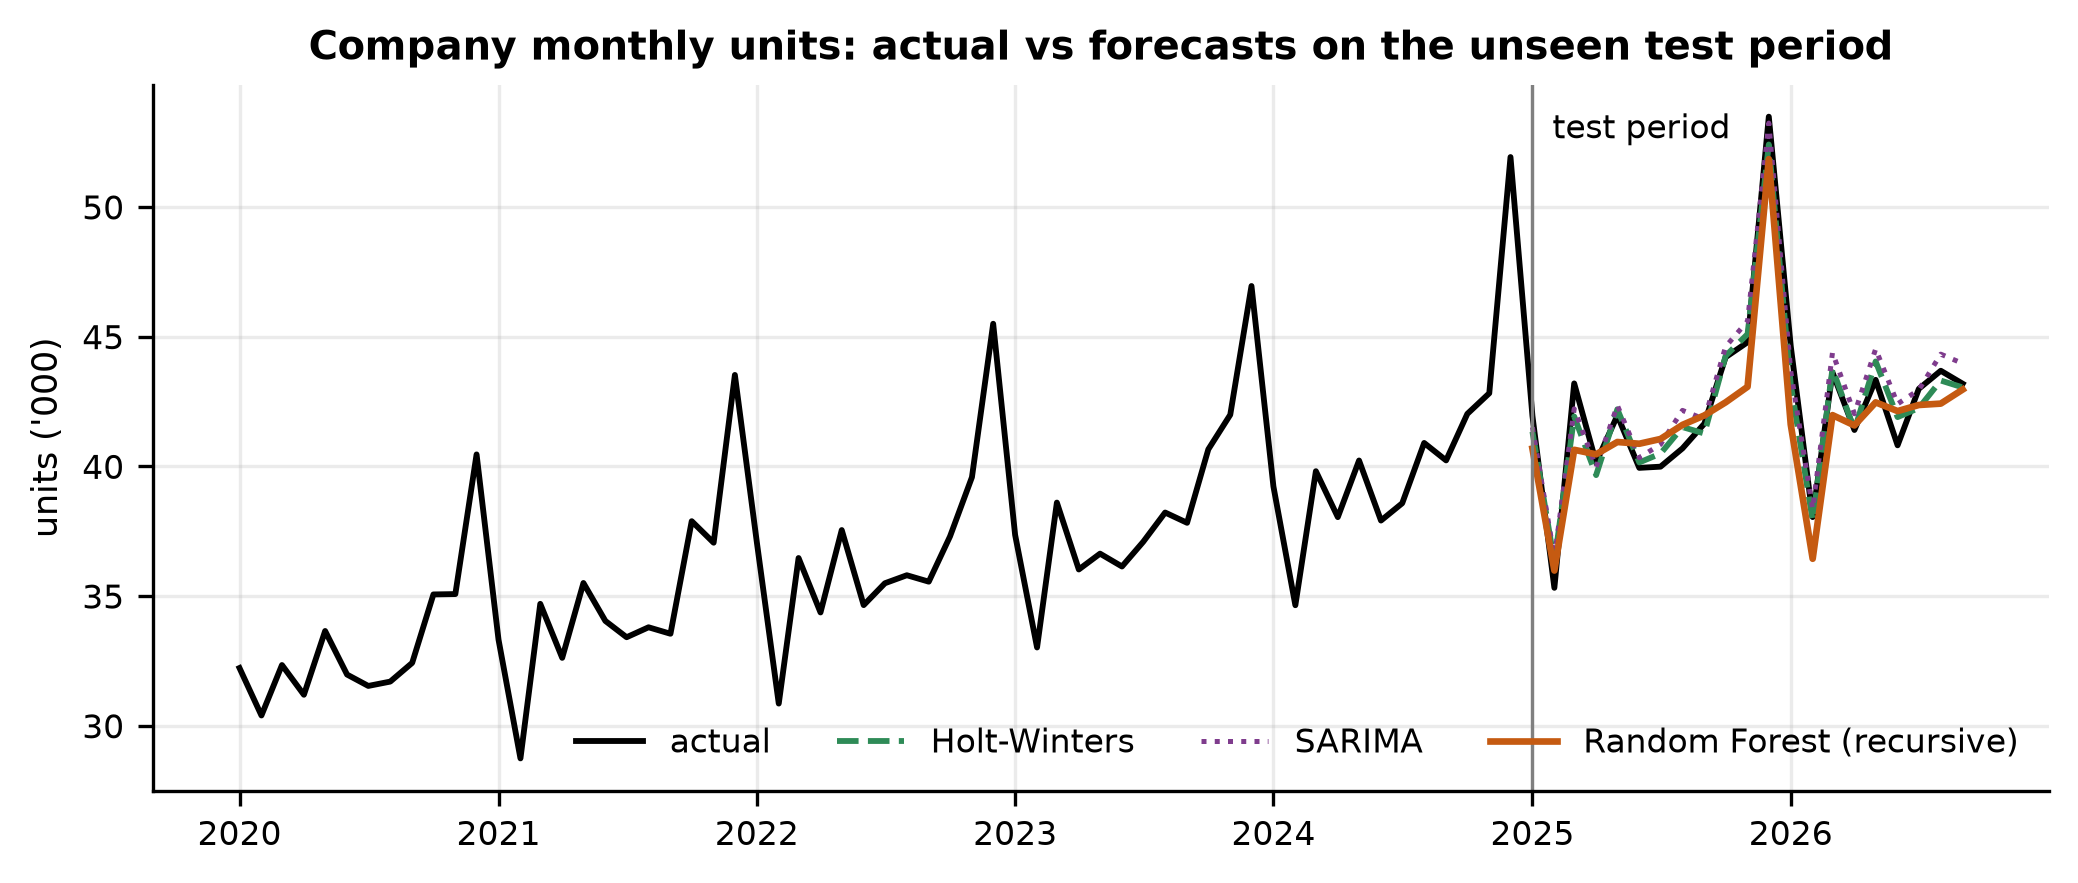
\includegraphics[width=\linewidth]{ml_company_forecast_test}
\caption{Company monthly units: actual values and competing forecasts over the test period}\label{fig:companyfc}
\end{figure}

\subsection{What drives the forecasts?}
\Cref{fig:importance} explains the models. For \BestReg, permutation importance shows that recent history
(lags and rolling means) carries most of the information, followed by seasonal features. The XGBoost SHAP values
give the same picture and also highlight the December indicator and the 12-month lag, which capture the
seasonal peak. The price features have little influence. This matches the near-zero price elasticity found in
\cref{ch:eda}, so the models and the explanatory analysis tell a consistent story.

\begin{figure}[htbp]\centering
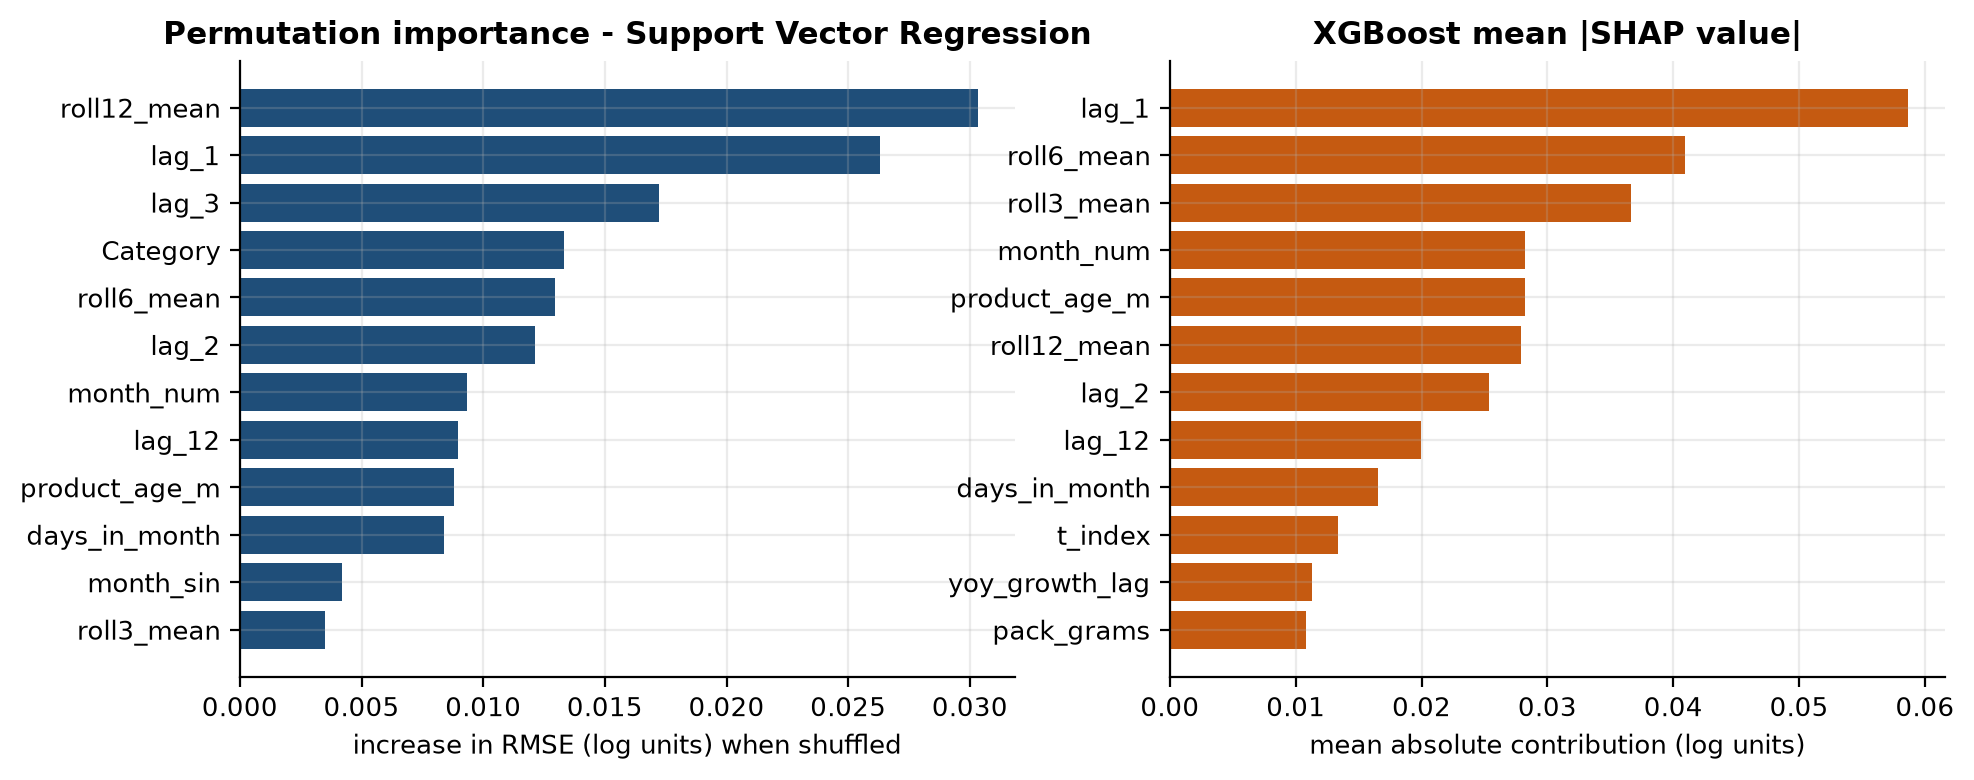
\includegraphics[width=\linewidth]{ml_feature_importance}
\caption{Permutation importance for the best forecasting model (left) and mean absolute SHAP values for XGBoost (right)}\label{fig:importance}
\end{figure}

\subsection{Twelve-month outlook}
The selected models were refitted on all data up to September 2026 and used to forecast October 2026 --
September 2027 (\cref{tab:future}, \cref{fig:future}). Net sales for these twelve months are forecast at
\BDT\FutSales million, with an 80\% interval from \FutSalesLo to \FutSalesHi million. That is \FutGrowth\% more
than the previous twelve months (\BDT\PrevSales million). Units are expected to change by \FutUnitsGrowth\%, and
the December peak is expected to recur. \FutTopCategory remains the largest category in the forecast. This
outlook can feed directly into the production, procurement and budgeting processes.

\begin{table}[htbp]
\centering
\footnotesize
\caption{Twelve-month forward forecast, October 2026 -- September 2027}
\label{tab:future}
\begin{adjustbox}{max width=\linewidth}
\begin{tabular}{lrrrrrrr}
\toprule
\textbf{Month} & \textbf{Units ML raw} & \textbf{Units (final)} & \textbf{80\% low} & \textbf{80\% high} & \textbf{Net sales (M)} & \textbf{80\% low } & \textbf{80\% high } \\
\midrule
Oct 2026 & 43,531 & 46,203 & 45,021 & 47,478 & 6.08 & 5.83 & 6.34 \\
Nov 2026 & 44,109 & 47,015 & 45,744 & 48,272 & 6.19 & 5.90 & 6.47 \\
Dec 2026 & 53,219 & 54,939 & 53,383 & 56,313 & 7.27 & 6.89 & 7.63 \\
Jan 2027 & 43,375 & 45,461 & 44,209 & 46,738 & 6.58 & 6.22 & 6.95 \\
Feb 2027 & 37,348 & 39,411 & 38,347 & 40,460 & 5.68 & 5.36 & 6.02 \\
Mar 2027 & 43,561 & 45,883 & 44,660 & 47,104 & 6.56 & 6.16 & 6.96 \\
Apr 2027 & 41,747 & 43,288 & 42,136 & 44,485 & 6.21 & 5.83 & 6.62 \\
May 2027 & 43,224 & 45,767 & 44,576 & 47,013 & 6.44 & 6.02 & 6.88 \\
Jun 2027 & 41,784 & 43,454 & 42,324 & 44,667 & 6.16 & 5.75 & 6.61 \\
Jul 2027 & 42,815 & 44,111 & 42,962 & 45,304 & 6.27 & 5.84 & 6.74 \\
Aug 2027 & 42,884 & 45,082 & 43,902 & 46,342 & 6.46 & 5.99 & 6.95 \\
Sep 2027 & 43,340 & 44,976 & 43,746 & 46,142 & 6.38 & 5.89 & 6.88 \\
\bottomrule
\end{tabular}
\end{adjustbox}
\par\smallskip\parbox{0.92\linewidth}{\footnotesize\emph{Note:} Units ML raw = sum of the Random Forest product forecasts before reconciliation. Final totals come from Holt-Winters models of company units and net sales (BDT million); intervals are the 10th and 90th percentiles of 2,000 simulated future paths. Product forecasts are scaled to these totals.}
\end{table}

\begin{figure}[htbp]\centering
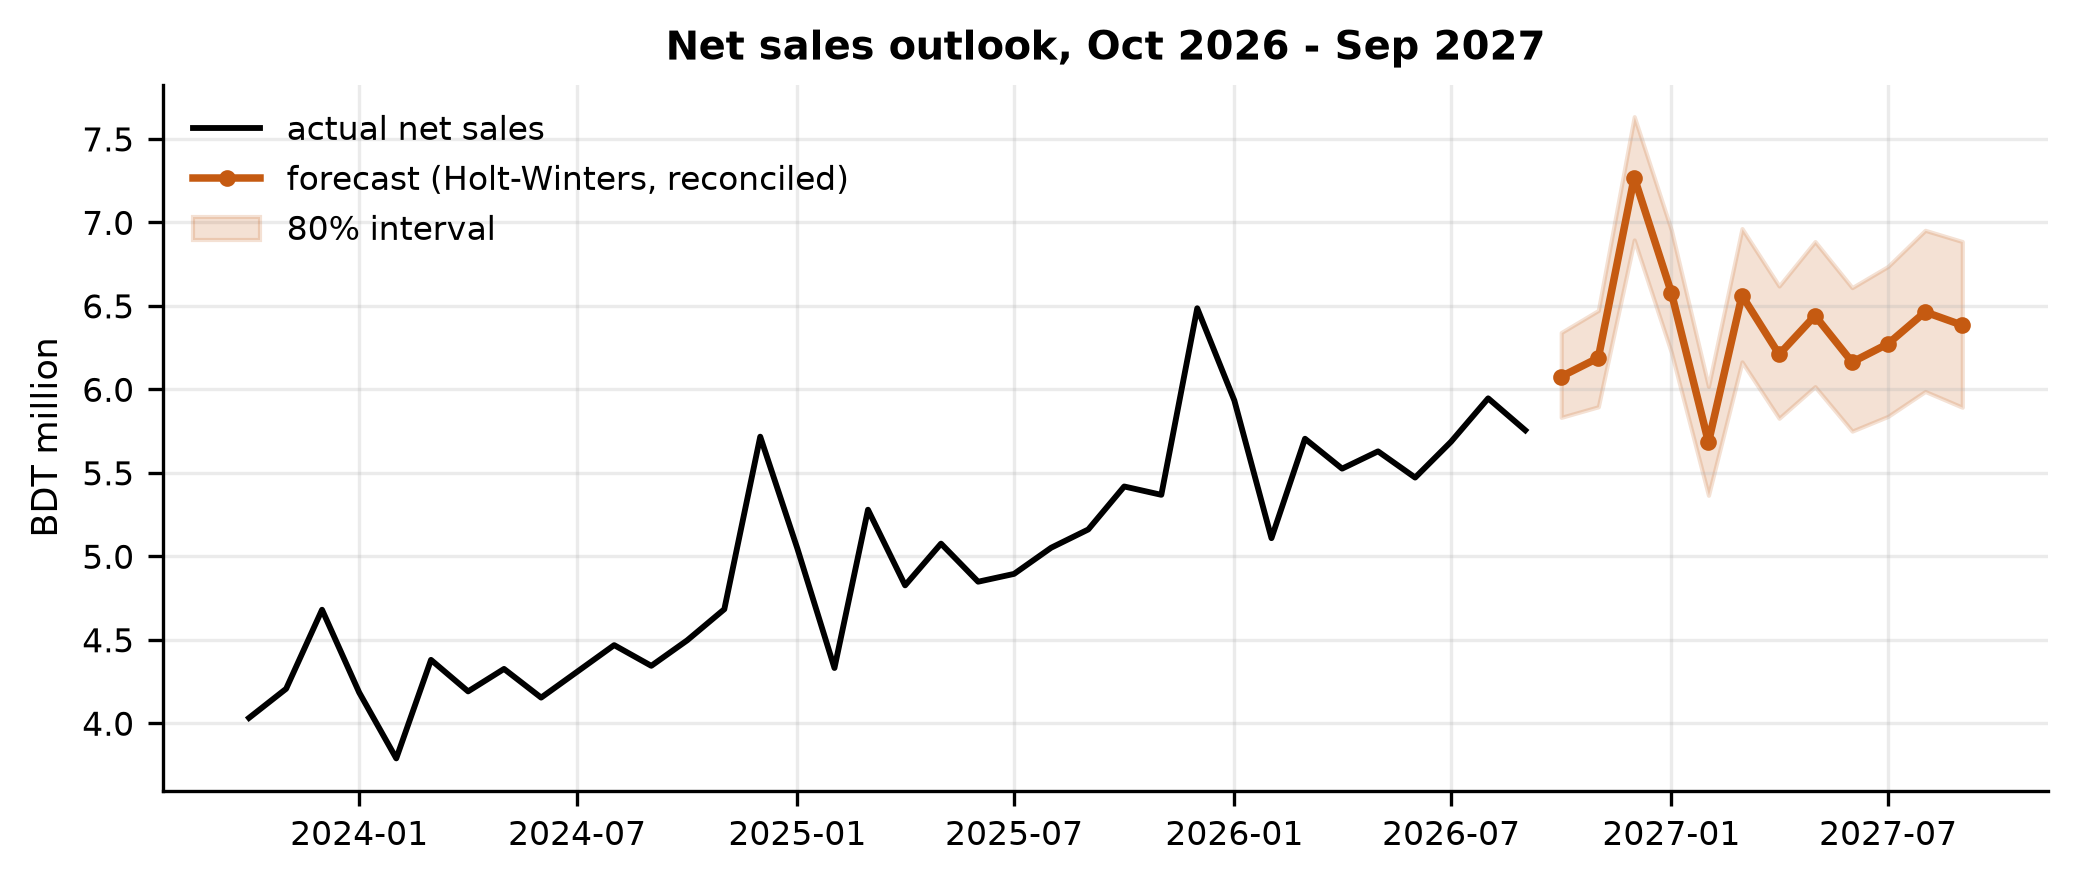
\includegraphics[width=\linewidth]{ml_future_forecast}
\caption{Net sales outlook for October 2026 -- September 2027 with 80\% prediction interval}\label{fig:future}
\end{figure}

\section{Large-order classification}
The classifier predicts, from information available when an order is entered, whether the order will contain
at least 10 units. Large orders made up \ClsPosTrain\% of training orders and \ClsPosTest\% of test orders. The
models were trained on \ClsTrain orders (2020--2024) and tested on \ClsTest orders (2025--2026). The features
were channel, region, customer type, category, price, discount, pack size, product age and calendar variables,
plus smoothed target encodings of channel $\times$ region and of product.

\begin{table}[htbp]
\centering
\footnotesize
\caption{Large-order classification ($\geq$10 units): test-set performance, 2025--2026}
\label{tab:classification}
\begin{adjustbox}{max width=\linewidth}
\begin{tabular}{lrrrrrrrrr}
\toprule
\textbf{Model} & \textbf{Accuracy} & \textbf{Precision} & \textbf{Recall} & \textbf{F1} & \textbf{ROC-AUC} & \textbf{PR-AUC} & \textbf{Threshold} & \textbf{Lift@10\%} & \textbf{Time (s)} \\
\midrule
Logistic Regression & 0.661 & 0.357 & 0.628 & 0.455 & 0.712 & 0.418 & 0.62 & 2.35 & 15 \\
Support Vector Machine (linear) & 0.629 & 0.341 & 0.698 & 0.458 & 0.711 & 0.417 & 0.31 & 2.34 & 42 \\
Gradient Boosting (hist) & 0.709 & 0.387 & 0.502 & 0.437 & 0.711 & 0.418 & 0.23 & 2.34 & 35 \\
Random Forest & 0.628 & 0.341 & 0.701 & 0.459 & 0.710 & 0.418 & 0.51 & 2.33 & 252 \\
XGBoost & 0.635 & 0.343 & 0.676 & 0.455 & 0.709 & 0.416 & 0.20 & 2.34 & 60 \\
Decision Tree & 0.550 & 0.309 & 0.807 & 0.447 & 0.709 & 0.407 & 0.48 & 2.31 & 14 \\
K-Nearest Neighbors & 0.634 & 0.333 & 0.624 & 0.434 & 0.684 & 0.396 & 0.20 & 2.28 & 73 \\
\bottomrule
\end{tabular}
\end{adjustbox}
\par\smallskip\parbox{0.92\linewidth}{\footnotesize\emph{Note:} Positive rate in the test years: 22.5\%; a classifier that always predicts `not large' would reach 77.5\% accuracy, so accuracy alone is misleading. Thresholds maximise F1 on the 2024 validation year. KNN uses a 60,000-row training sample. Lift@10\% is the large-order rate among the 10\% highest-scored orders divided by the overall rate.}
\end{table}

\Cref{tab:classification} and \cref{fig:classification} show a clear and instructive result. All seven
algorithms reach almost the same ROC-AUC, between \ClsAUCmin and \ClsAUC, and \ClsBest is the best. The model
that always predicts ``not large'' would be \ClsMajority\% accurate yet useless. The tuned models instead
recover most large orders (recall about \ClsRecall for \ClsBest) at moderate precision. Ranked by score, the top
10\% of orders contain large orders \ClsLift times more often than average. The ceiling is set by the
\emph{information} in the data, not by the algorithm. XGBoost (\ClsXGBAUC) gains nothing over logistic
regression, and KNN (\ClsKNNAUC) is weakest because distances become uninformative over many one-hot features.

\begin{figure}[htbp]\centering
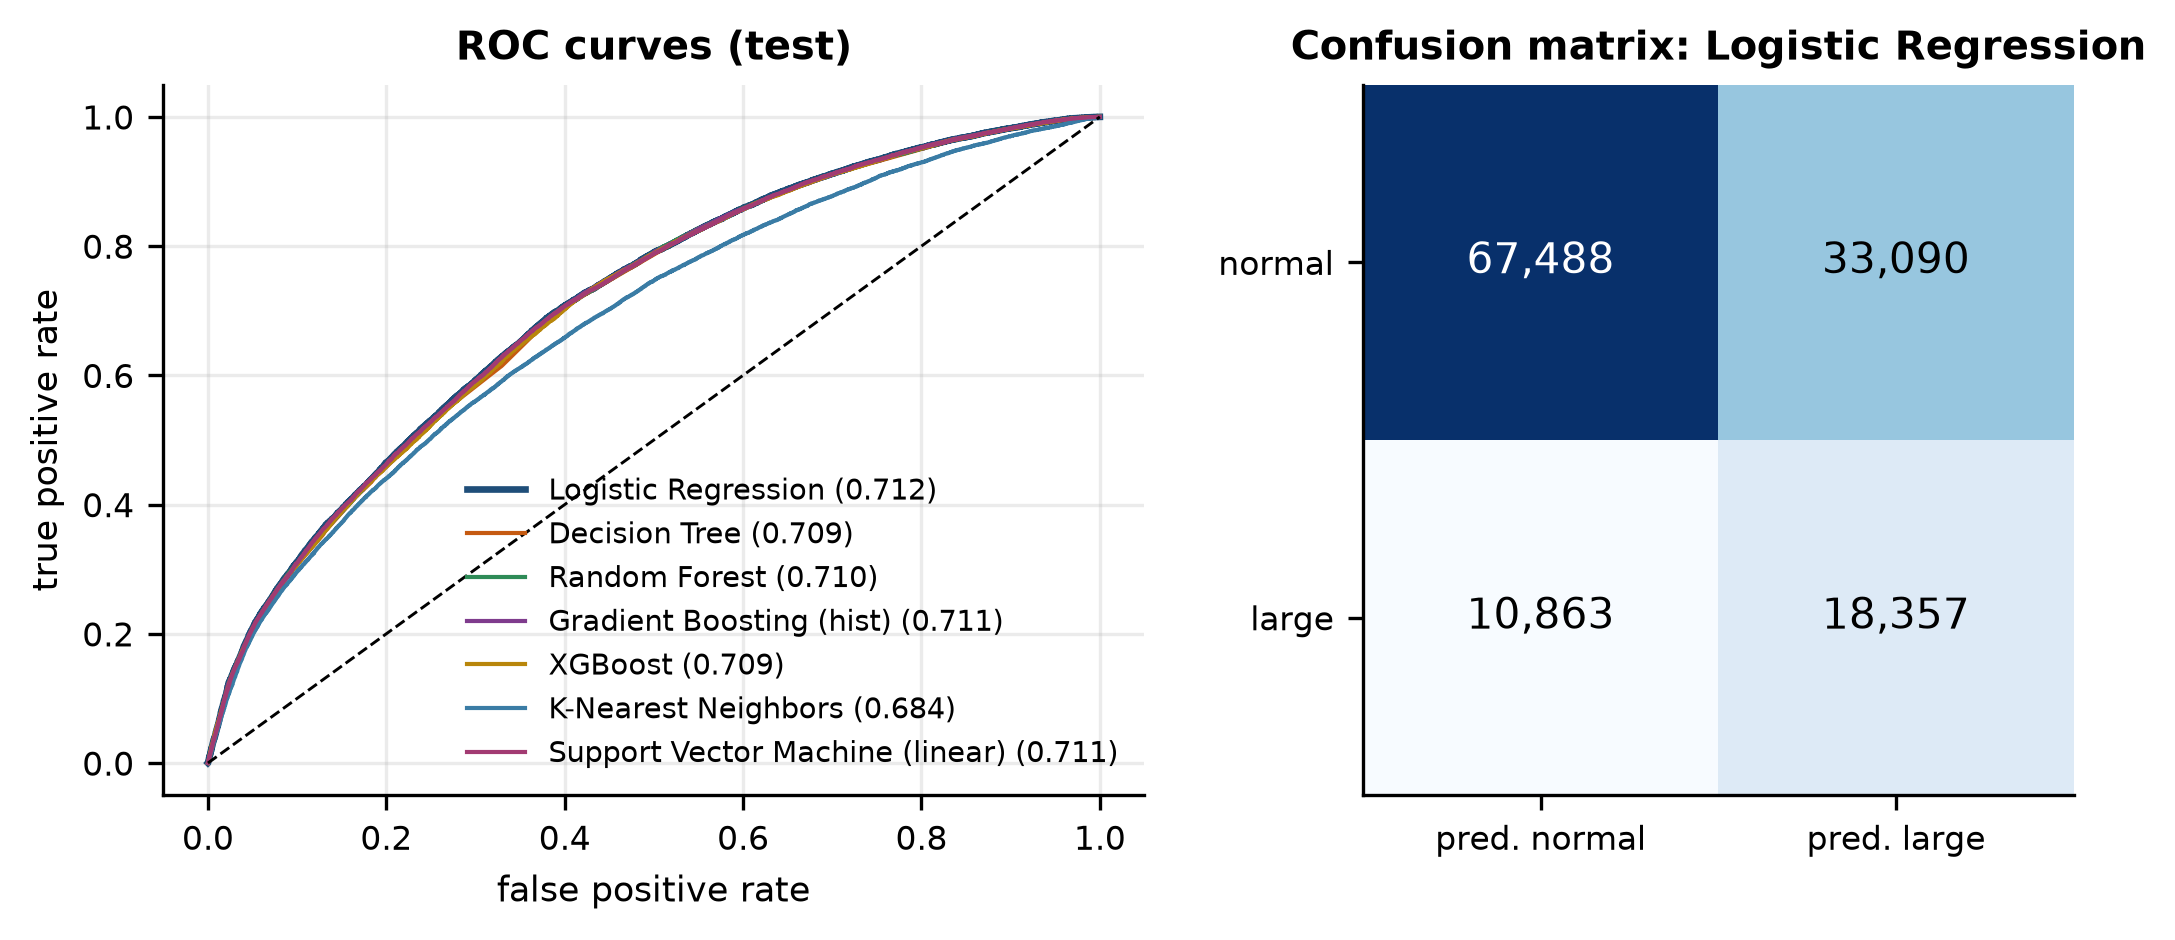
\includegraphics[width=\linewidth]{ml_classification}
\caption{ROC curves (left), confusion matrix of the best model (centre) and metric comparison (right) for large-order classification}\label{fig:classification}
\end{figure}

The XGBoost gain importance (\cref{fig:clsimp}) identifies the reason. The sales channel accounts for about
\ClsChannelImp\% of the model's gain and region for about \ClsRegionImp\%. Product, price, discount and
calendar contribute very little. In the test years \LargeDist\% of distributor orders were large, against only
\LargeEcom\% of E-commerce orders. Order size within a channel and region is otherwise close to random. For
decision-making, then, the useful output is a \emph{channel-and-region-level} expectation of large orders for
logistics planning, rather than a precise order-by-order prediction.

\begin{figure}[htbp]\centering
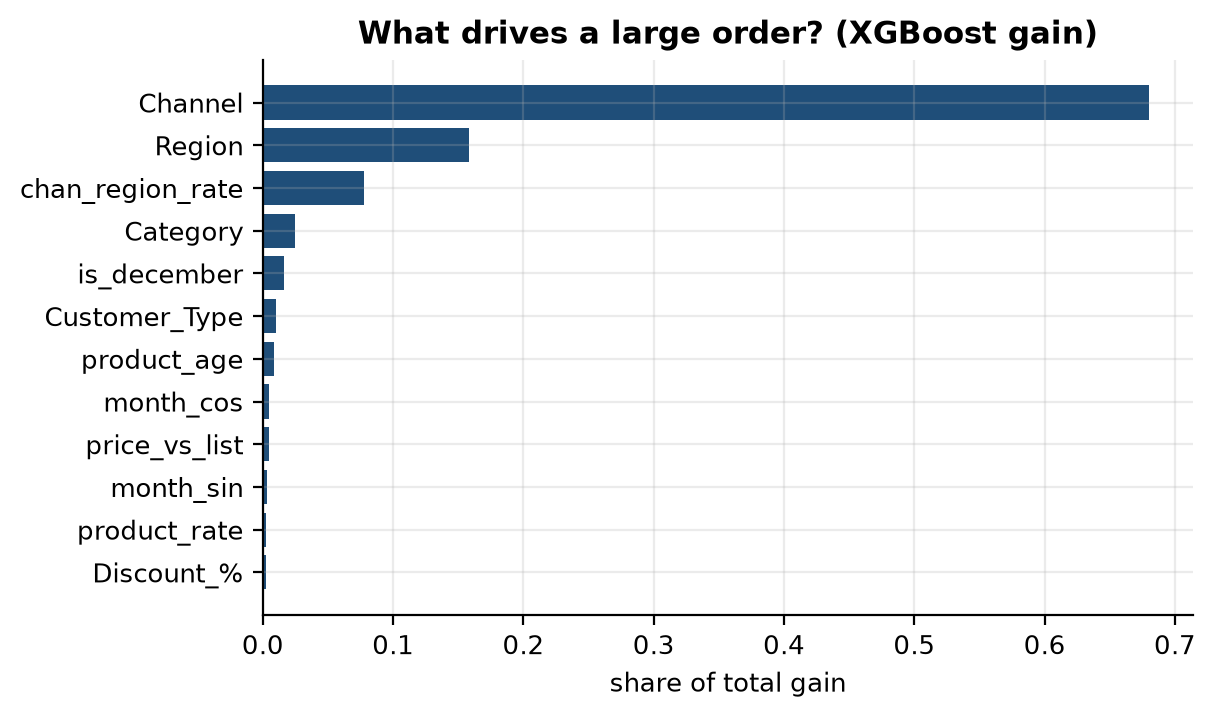
\includegraphics[width=.65\linewidth]{ml_classification_importance}
\caption{Drivers of large orders: XGBoost gain aggregated by original variable}\label{fig:clsimp}
\end{figure}

\section{Segmentation}
\subsection{Product portfolio}
Each product was described by its log revenue, log average price, unit growth from 2023 to 2025, December
seasonality index and month-to-month volatility. Order size and channel mix were excluded because they barely
vary between products (\cref{ch:eda}) and would only add noise. The features were standardised. $K$-Means,
agglomerative (Ward) and Gaussian-mixture clustering were compared for $k=2,\dots,8$
(\cref{fig:clustering}, \cref{tab:clustercompare}). Within the practical range of three to five segments,
$K$-Means with $k=\ProdK$ gave the best silhouette (\ProdSil) and a Davies--Bouldin index of \ProdDB. The
resulting segments are summarised in \cref{tab:productclusters} and named automatically from their averages.

\begin{table}[htbp]
\centering
\small
\caption{Product portfolio segments (K-Means, k=5)}
\label{tab:productclusters}
\begin{adjustbox}{max width=\linewidth}
\begin{tabular}{lrrrrrr}
\toprule
\textbf{Segment} & \textbf{Products} & \textbf{Sales share \%} & \textbf{Avg price} & \textbf{Units/order} & \textbf{Unit growth \%/yr} & \textbf{Dec. index} \\
\midrule
Premium \& gift packs & 13 & 33.3 & 156 & 6.24 & +7.8 & 123 \\
Mature slow-growth lines & 13 & 31.9 & 130 & 6.17 & +2.3 & 120 \\
Core family packs & 11 & 28.1 & 133 & 6.17 & +4.9 & 134 \\
Single-serve value packs & 9 & 4.2 & 23 & 6.22 & +6.0 & 119 \\
Niche \& new lines & 6 & 2.5 & 24 & 6.22 & +4.0 & 134 \\
\bottomrule
\end{tabular}
\end{adjustbox}
\par\smallskip\parbox{0.92\linewidth}{\footnotesize\emph{Note:} Growth is the compound annual growth of units between 2023 and 2025. December index = average December units relative to the product's average month (100 = no seasonality).}
\end{table}

\subsection{Market segments}
The 220 combinations of region, channel and customer type were clustered on their revenue, average order
value, units per order, price, discount, growth and gift-pack share. $K$-Means selected $k=\MktK$ segments
(silhouette \MktSil). They separate clearly into \emph{core retail trade} (General and Modern Trade in the large
cities), \emph{bulk distribution}, small-ticket \emph{online and regional} cells, and a group of
\emph{emerging high-growth} cells (\cref{tab:marketclusters}).

\begin{table}[htbp]
\centering
\scriptsize
\caption{Market segments of region $\times$ channel $\times$ customer-type cells (K-Means, k=4)}
\label{tab:marketclusters}
\begin{adjustbox}{max width=\linewidth}
\begin{tabular}{lrrrrrll}
\toprule
\textbf{Segment} & \textbf{Cells} & \textbf{Sales share \%} & \textbf{AOV (BDT)} & \textbf{Units/order} & \textbf{Growth \%/yr} & \textbf{Main channels} & \textbf{Main regions} \\
\midrule
Core retail trade & 99 & 71.9 & 518 & 5.02 & +14.8 & General Trade, Modern Trade & Dhaka, Chattogram, Gazipur \\
Bulk distribution & 52 & 22.6 & 966 & 9.96 & +16.2 & Distributor & Chattogram, Dhaka, Gazipur \\
Small-ticket online \& regional & 50 & 4.2 & 341 & 3.43 & +16.7 & E-commerce, Modern Trade & Barishal, Khulna, Rajshahi \\
Emerging high-growth cells & 19 & 1.3 & 431 & 4.16 & +33.2 & E-commerce, Modern Trade & Cumilla, Khulna, Mymensingh \\
\bottomrule
\end{tabular}
\end{adjustbox}
\end{table}
\begin{table}[htbp]
\centering
\small
\caption{Comparison of clustering algorithms at the selected number of clusters}
\label{tab:clustercompare}
\begin{adjustbox}{max width=\linewidth}
\begin{tabular}{llrrrr}
\toprule
\textbf{Problem} & \textbf{Algorithm} & \textbf{k} & \textbf{Silhouette} & \textbf{Davies-Bouldin} & \textbf{Calinski-Harabasz} \\
\midrule
Products & K-Means & 5 & 0.237 & 1.271 & 16.2 \\
Products & Agglomerative (Ward) & 5 & 0.212 & 1.195 & 14.9 \\
Products & Gaussian Mixture & 5 & 0.233 & 1.237 & 15.3 \\
Market cells & K-Means & 4 & 0.243 & 1.497 & 54.2 \\
Market cells & Agglomerative (Ward) & 4 & 0.250 & 1.467 & 48.9 \\
Market cells & Gaussian Mixture & 4 & 0.165 & 1.753 & 42.4 \\
\bottomrule
\end{tabular}
\end{adjustbox}
\par\smallskip\parbox{0.92\linewidth}{\footnotesize\emph{Note:} Higher silhouette and Calinski--Harabasz and lower Davies--Bouldin values indicate better-separated clusters.}
\end{table}

\begin{figure}[htbp]\centering
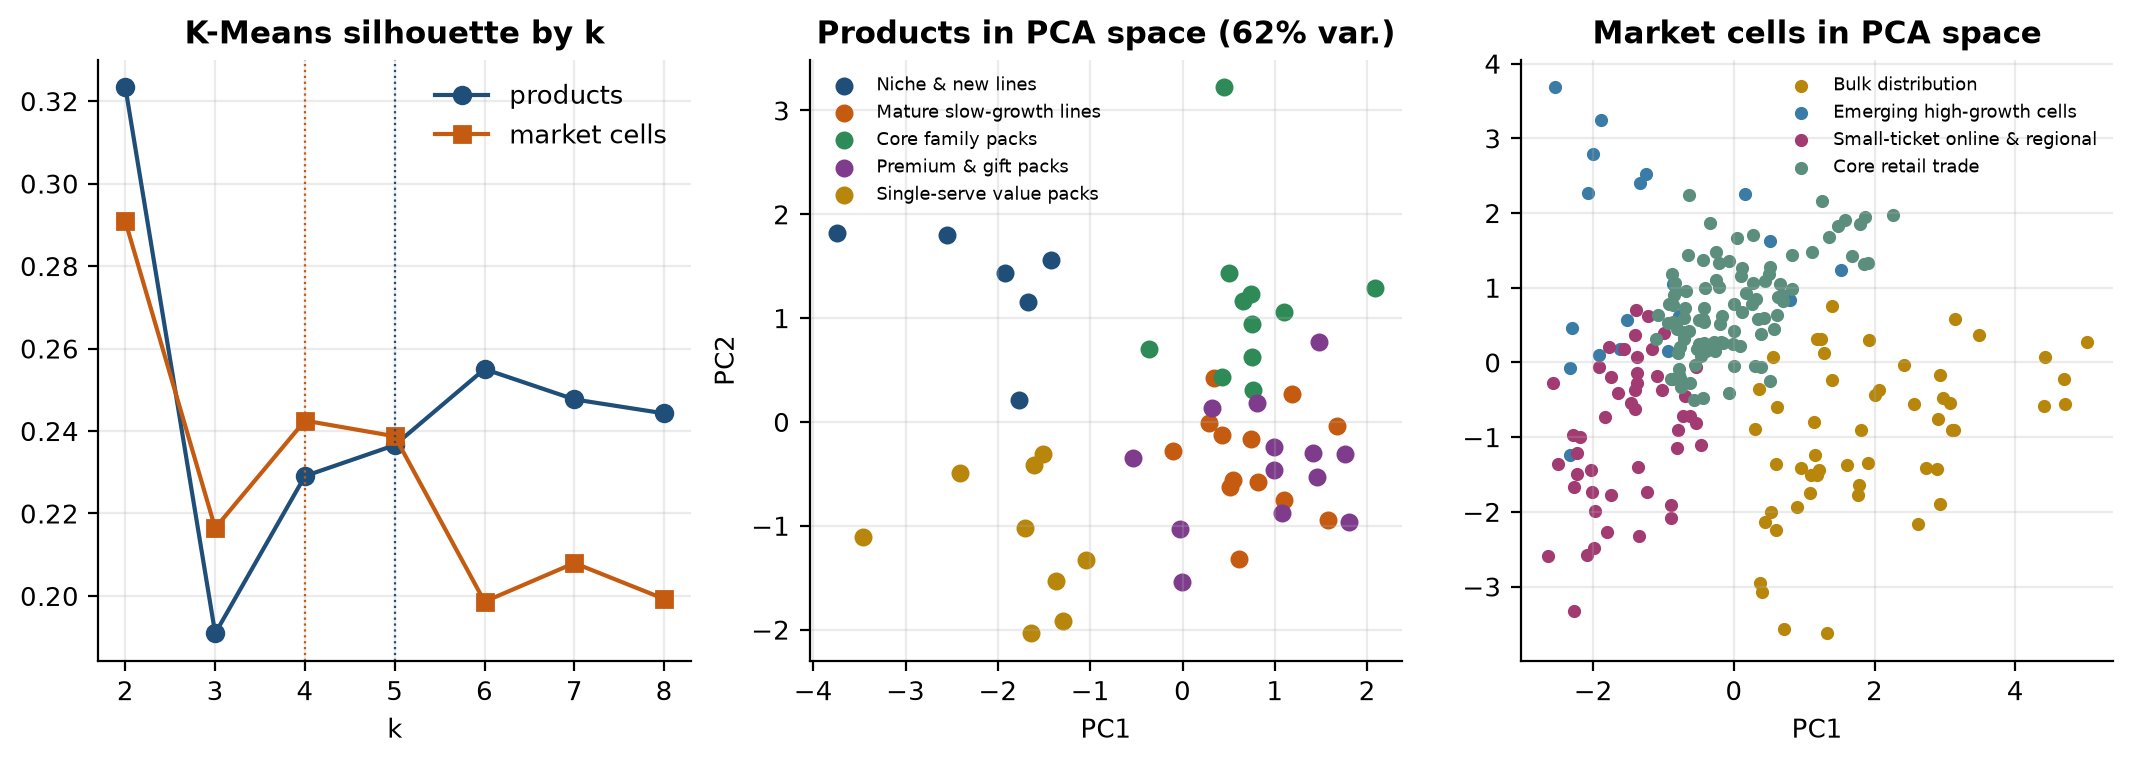
\includegraphics[width=\linewidth]{ml_clustering}
\caption{Silhouette score by number of clusters (left); products (centre) and market cells (right) projected onto the first two principal components}\label{fig:clustering}
\end{figure}

The silhouette values (\ProdSil and \MktSil) indicate weak to moderate structure \citep{rousseeuw1987}. The
segments are therefore useful summaries for strategy, not sharply separated natural groups. $K$-Means and Ward
clustering agreed closely, while Gaussian mixtures performed worst on these small samples. This ranking is
reported so that a reader can judge the robustness of the segmentation.

\section{Anomaly detection}
\subsection{Daily monitoring}
For each day, an expected value was computed as a 31-day centred rolling median multiplied by the month-of-year
seasonal factor. Deviations were scored on the log scale with the robust $z$-score
$z = 0.6745\,(r-\tilde r)/\text{MAD}$ and, separately, with an Isolation Forest over four daily features.
Together the two methods flagged \AnomDays of the 2,465 trading days: \AnomDaysZ by the robust $z$-score and
\AnomDaysIF by the Isolation Forest (\cref{fig:anomdaily}, \cref{tab:dailyanom}). Most flagged days are
unusually weak trading days. In a live deployment each would be checked against known causes such as public
holidays, strikes or system outages.

\begin{figure}[htbp]\centering
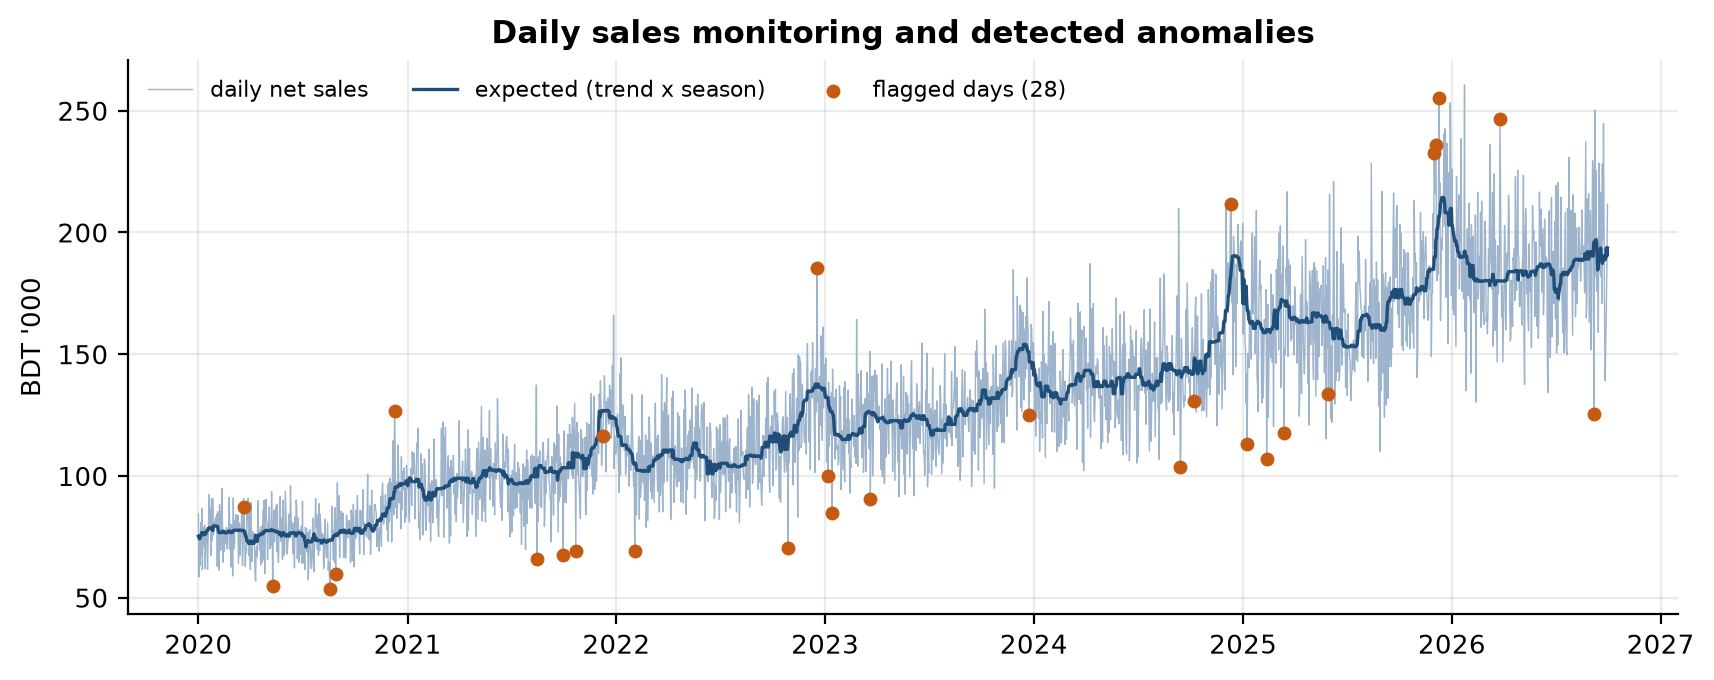
\includegraphics[width=\linewidth]{anomaly_daily}
\caption{Daily net sales, expected level and detected anomalies}\label{fig:anomdaily}
\end{figure}
\begin{table}[htbp]
\centering
\small
\caption{Ten most unusual trading days (seasonally adjusted)}
\label{tab:dailyanom}
\begin{adjustbox}{max width=\linewidth}
\begin{tabular}{lrrrrl}
\toprule
\textbf{Date} & \textbf{Net sales (BDT)} & \textbf{Expected (BDT)} & \textbf{Deviation \%} & \textbf{Robust z} & \textbf{Flagged by} \\
\midrule
28 Oct 2022 & 70,215 & 113,462 & -38.1 & -4.01 & robust z \\
22 Oct 2021 & 69,194 & 109,276 & -36.7 & -3.82 & robust z \\
06 Sep 2026 & 125,262 & 195,913 & -36.1 & -3.74 & robust z \\
30 Sep 2021 & 67,358 & 103,385 & -34.8 & -3.58 & both \\
02 Feb 2022 & 69,149 & 104,763 & -34.0 & -3.47 & Isolation Forest \\
15 Aug 2021 & 66,039 & 99,664 & -33.7 & -3.44 & Isolation Forest \\
11 Feb 2025 & 106,843 & 160,093 & -33.3 & -3.38 & Isolation Forest \\
13 Jan 2023 & 84,814 & 126,483 & -32.9 & -3.34 & Isolation Forest \\
08 Jan 2025 & 113,188 & 168,043 & -32.6 & -3.31 & Isolation Forest \\
13 Mar 2025 & 117,699 & 171,855 & -31.5 & -3.17 & Isolation Forest \\
\bottomrule
\end{tabular}
\end{adjustbox}
\end{table}

\subsection{Transaction screening}
Without labelled errors, a detector's ability cannot be measured on the real data. Following the approach of
the preprocessing scripts, 1,000 realistic errors of four types (250 each) were therefore planted in a copy of
the 500,000 orders (\cref{tab:anomaly}). The per-product IQR rule on quantity detected only \AnomIQRRecall\% of
the planted errors, because three of the four error types do not involve quantity. Simple business rules on
price and discount caught \AnomRuleRecall\% with perfect precision but missed every quantity error. The
Isolation Forest caught \AnomIFRecall\% across all four types. Price and discount errors were found completely,
and most inflated quantities were found too. The lesson is that rules and machine learning are complementary.
Rules are precise for known failure modes, and the Isolation Forest provides broad coverage for unknown ones.

\begin{table}[htbp]
\centering
\footnotesize
\caption{Detection of 1,000 injected transaction errors in 500,000 orders}
\label{tab:anomaly}
\begin{adjustbox}{max width=\linewidth}
\begin{tabular}{lrrrrrrr}
\toprule
\textbf{Method} & \textbf{Flagged} & \textbf{Precision} & \textbf{Recall} & \textbf{Price x10} & \textbf{Qty x20} & \textbf{Disc. 30-45\%} & \textbf{Price 10\%} \\
\midrule
IQR on log quantity (per product) & 1,500 & 0.112 & 0.168 & 0.00 & 0.66 & 0.00 & 0.01 \\
Business rules (price, discount) & 750 & 1.000 & 0.750 & 1.00 & 0.00 & 1.00 & 1.00 \\
Isolation Forest (4 features) & 2,500 & 0.364 & 0.909 & 1.00 & 0.64 & 1.00 & 1.00 \\
Rules OR Isolation Forest & 2,500 & 0.364 & 0.909 & 1.00 & 0.64 & 1.00 & 1.00 \\
\bottomrule
\end{tabular}
\end{adjustbox}
\par\smallskip\parbox{0.92\linewidth}{\footnotesize\emph{Note:} The last four columns give the share of each error type that was detected. 250 errors of each type were planted in a copy of the data.}
\end{table}

\section{Summary of model evaluation}
\begin{table}[htbp]\centering\small
\caption{Summary of the selected model for each analytical problem}\label{tab:modelsummary}
\begin{tabularx}{\linewidth}{@{}lXl@{}}
\toprule
\textbf{Problem} & \textbf{Selected approach} & \textbf{Key test result} \\ \midrule
Product demand (1-step) & \BestReg & WAPE \BestRegWAPE\%, $R^2$ \BestRegRtwo \\
Product demand (multi-step) & \BestRec, recursive & WAPE \BestRecWAPE\% \\
Company total & Holt--Winters + top-down reconciliation & MAPE \HWMAPE\% \\
Large orders & \ClsBest & ROC-AUC \ClsAUC, lift \ClsLift \\
Product segments & $K$-Means, $k=\ProdK$ & silhouette \ProdSil \\
Market segments & $K$-Means, $k=\MktK$ & silhouette \MktSil \\
Transaction anomalies & rules OR Isolation Forest & recall \AnomComboRecall\% \\ \bottomrule
\end{tabularx}
\end{table}
As the proposal required, models were selected on appropriate metrics \emph{and} business relevance, not on
accuracy alone. Where a simpler model performed as well as a complex one, as with logistic regression versus
XGBoost for classification, the simpler and more interpretable model is preferred.

\chapter[Dashboard, Deployment and Decision Support]{Business Intelligence Dashboard,\\ Deployment and Decision Support}\label{ch:dashboard}

\section{Design goals}
The dashboard is where the framework meets its users, the sales, supply-chain and senior managers. Following
\citet{few2013}, \citet{tufte2001} and \citet{knaflic2015}, it was designed to meet five requirements:
\begin{enumerate}
  \item \textbf{At-a-glance KPIs}: net sales, units, orders, average order value, discount rate and
        year-to-date growth appear at the top of the overview page;
  \item \textbf{Consistent filtering}: one set of filters (years, region, channel, customer type, category)
        applies across all pages;
  \item \textbf{The three management questions}: pages progress from \emph{what happened} (overview, trends,
        products, markets) to \emph{why} (drivers, segments) and \emph{what next} (forecast, anomalies,
        recommendations);
  \item \textbf{Honest presentation}: forecasts are always shown with prediction intervals, model accuracy is
        visible to users, and colour is used only to encode meaning. Following \citet{tufte2001}, decoration
        that carries no data (3-D effects, gauges, heavy grid lines) is avoided;
  \item \textbf{Free and accessible}: the dashboard runs in any web browser and is hosted at no cost.
\end{enumerate}

\section{Implementation}
The dashboard was built with Streamlit and Plotly in a single Python file (\path{dashboard/app.py}). It does
not read the 500,000 raw rows. It reads compact aggregates produced by the pipeline: a monthly cube by region
$\times$ channel $\times$ customer type $\times$ category, monthly product-by-region totals, forecasts, model
scores, segment tables and anomaly lists. Their total size is about 2~MB, so the application starts in seconds
on the free hosting tier, while every filter combination remains exact. Data are cached in memory after the
first load. Each page has its own web address (for example \path{?page=forecast}), so a manager can bookmark
or share a specific view. \Cref{tab:pages} lists the nine pages, and
\cref{fig:dashoverview,fig:dashtrends,fig:dashproducts,fig:dashmarkets,fig:dashforecast,fig:dashmodels,fig:dashanomalies,fig:dashinsights,fig:dashquality}
show each of them as deployed. All screenshots were captured automatically from the running application by
\path{tools/capture_screenshots.py}, so they can be refreshed whenever the data change.

\begin{table}[htbp]\centering\small
\caption{Pages of the interactive dashboard}\label{tab:pages}
\begin{tabularx}{\linewidth}{@{}lX@{}}
\toprule
\textbf{Page} & \textbf{Content} \\ \midrule
Executive overview & KPI cards, monthly sales with moving average, category, region and channel mix, annual table \\
Trends \& seasonality & Stacked trends by any dimension, year $\times$ month heat map, seasonal index, year-on-year lines \\
Products \& portfolio & Top-$N$ products, Pareto/ABC analysis, ML product segments, single-product drill-down \\
Markets \& customers & Region $\times$ channel heat maps, customer types, regional CAGR, ML market segments \\
Demand forecast & 12-month outlook with interval, category and product forecasts, model leaderboard, CSV download \\
Machine-learning models & Regression, classification and clustering results with feature importance \\
Anomaly monitor & Daily sales against expected level with flagged days; most suspicious orders \\
Insights \& recommendations & Automatically generated insights with recommended actions \\
Data quality \& method & Validation report, cleaning log and architecture diagram \\ \bottomrule
\end{tabularx}
\end{table}

\section{Walk-through of the dashboard}
\paragraph{What happened.} The \emph{executive overview} (\cref{fig:dashoverview}) opens with six KPI cards and
the monthly sales trend with its 12-month average. Below them, the category, region and channel mix and an
annual summary table answer the first questions a manager asks. The \emph{trends} page
(\cref{fig:dashtrends}) shows how any dimension develops over time and makes the December peak and February
trough visible in a year~$\times$~month heat map. The \emph{products} page (\cref{fig:dashproducts}) ranks the
products, draws the Pareto curve with ABC classes and lets the user drill down into a single product. The
\emph{markets} page (\cref{fig:dashmarkets}) compares regions, channels and customer types and shows the
market segments found by clustering.

\paragraph{What next.} The \emph{demand forecast} page (\cref{fig:dashforecast}) presents the 12-month outlook
with its 80\% prediction interval, forecasts by category and product, and the leaderboard of forecasting
models. The forecasts can be downloaded as CSV for the production plan. The \emph{machine-learning} page
(\cref{fig:dashmodels}) exposes the evidence behind the forecasts: test errors of all models against the
baselines, the recursive multi-step test and feature importance, plus the classification and clustering
results in separate tabs.

\paragraph{Control and action.} The \emph{anomaly monitor} (\cref{fig:dashanomalies}) plots daily sales against
the expected level, marks the flagged days and lists the most suspicious orders for checking. The
\emph{insights} page (\cref{fig:dashinsights}) turns all results into plain-language findings, each followed by
a recommended action. Finally, the \emph{data quality} page (\cref{fig:dashquality}) documents the validation
checks and the cleaning log, so users can see why the numbers can be trusted.

\newcommand{\dashshot}[3]{%
\begin{figure}[p]\centering
\includegraphics[width=\linewidth,height=.86\textheight,keepaspectratio]{screens/#1}
\caption{#2}\label{#3}
\end{figure}}

\dashshot{dash_overview}{Dashboard page 1 -- Executive overview: KPI cards, monthly trend, sales mix and annual summary}{fig:dashoverview}
\dashshot{dash_trends_main}{Dashboard page 2 -- Trends and seasonality}{fig:dashtrends}
\dashshot{dash_products_main}{Dashboard page 3 -- Products and portfolio, with Pareto/ABC analysis and product segments}{fig:dashproducts}
\dashshot{dash_markets_main}{Dashboard page 4 -- Markets and customers, with region $\times$ channel heat maps and market segments}{fig:dashmarkets}
\dashshot{dash_forecast_main}{Dashboard page 5 -- Demand forecast: 12-month outlook with its 80\% interval, category and product forecasts}{fig:dashforecast}
\dashshot{dash_models_main}{Dashboard page 6 -- Machine-learning models: test errors against baselines, recursive test and feature importance}{fig:dashmodels}
\dashshot{dash_anomalies_main}{Dashboard page 7 -- Anomaly monitor: daily sales against the expected level and suspicious orders}{fig:dashanomalies}
\dashshot{dash_insights_main}{Dashboard page 8 -- Automatically generated insights and recommendations}{fig:dashinsights}
\dashshot{dash_quality_main}{Dashboard page 9 -- Data quality and method}{fig:dashquality}

\section{Deployment and operation}\label{sec:deployment}
\subsection{Live system}
The complete project is publicly available on three free platforms (\cref{tab:links}). The source code is
version-controlled on GitHub. The interactive dashboard runs on Streamlit Community Cloud, and the project
website, which also serves this report as a PDF, is hosted on GitHub Pages. All three use HTTPS. The raw
transaction file is deliberately excluded from the public repository by \texttt{.gitignore}. Only the small,
aggregated files that the dashboard needs are published, and commits use a private GitHub e-mail address.

\begin{table}[htbp]\centering\small
\caption{Public addresses of the deployed system}\label{tab:links}
\begin{tabularx}{\linewidth}{@{}lXl@{}}
\toprule
\textbf{Component} & \textbf{Address} & \textbf{Platform} \\ \midrule
Interactive dashboard & \dashurl & Streamlit Community Cloud \\
Project website and PDF report & \siteurl & GitHub Pages \\
Source code and history & \repo & GitHub \\ \bottomrule
\end{tabularx}
\end{table}

\subsection{Continuous deployment}
Deployment is automatic (\cref{fig:cicd}). When a change is pushed to the \texttt{main} branch, Streamlit Cloud
rebuilds the dashboard from \path{dashboard/app.py} and its small \path{dashboard/requirements.txt}, and GitHub
Pages republishes the \path{docs/} folder. A new month of data therefore reaches managers through three steps:
re-run the pipeline, commit, and push. No server needs to be maintained. On the free tier, the dashboard sleeps
after several days without visitors and wakes in about half a minute on the next visit, which is acceptable for
a monthly planning tool.

\begin{figure}[htbp]\centering
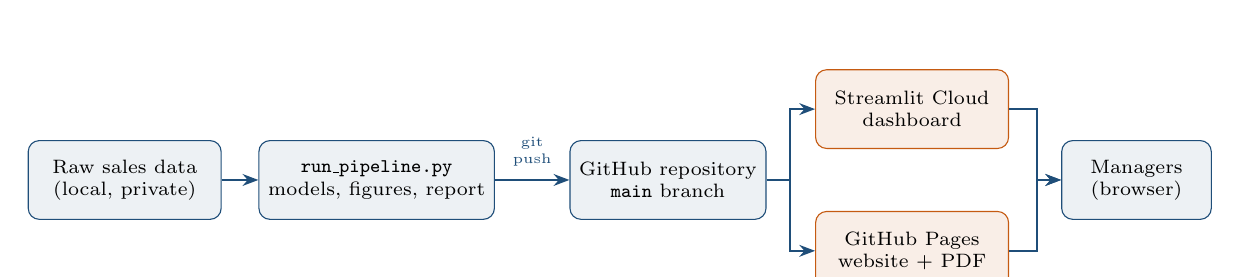
\begin{tikzpicture}[every node/.style={font=\scriptsize},
  box/.style={draw=brand, rounded corners, fill=brand!8, minimum width=2.45cm, minimum height=10mm, align=center},
  web/.style={box, draw=accent, fill=accent!10},
  arr/.style={-{Stealth[length=2mm]}, thick, brand}]
\node[box] (data) at (0,0) {Raw sales data\\(local, private)};
\node[box] (pipe) at (3.2,0) {\texttt{run\_pipeline.py}\\models, figures, report};
\node[box] (git)  at (6.9,0) {GitHub repository\\\texttt{main} branch};
\node[web] (st)   at (10.0,0.9) {Streamlit Cloud\\dashboard};
\node[web] (gp)   at (10.0,-0.9) {GitHub Pages\\website + PDF};
\node[box, minimum width=1.9cm] (users) at (12.85,0) {Managers\\(browser)};
\draw[arr] (data) -- (pipe);
\draw[arr] (pipe) -- node[above=0.5mm, align=center, font=\tiny]{git\\push} (git);
\draw[arr] (git.east) -- ++(0.3,0) |- (st.west);  \draw[arr] (git.east) -- ++(0.3,0) |- (gp.west);
\draw[arr] (st.east) -- ++(0.35,0) |- (users.west); \draw[arr] (gp.east) -- ++(0.35,0) |- (users.west);
\end{tikzpicture}
\caption{Continuous deployment: one push updates both the dashboard and the website}\label{fig:cicd}
\end{figure}

\begin{figure}[htbp]\centering
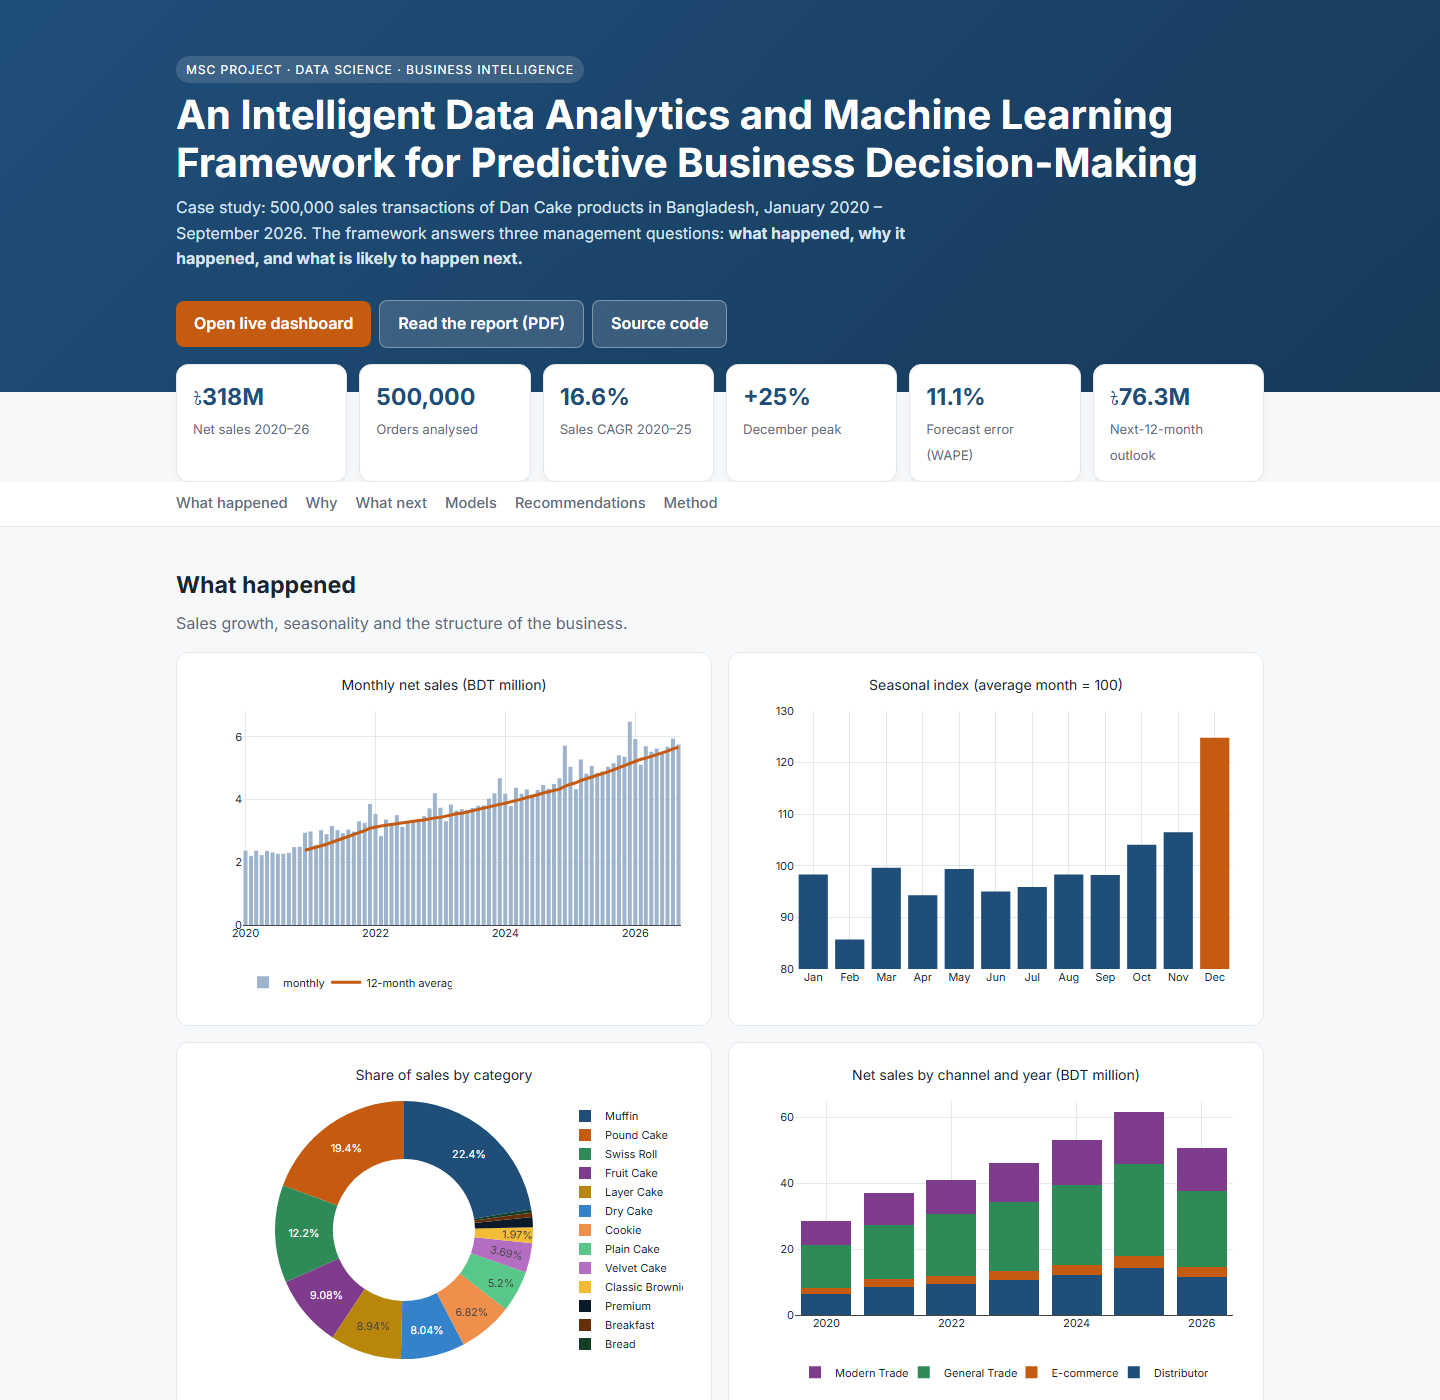
\includegraphics[width=\linewidth]{screens/website}
\caption{Project website on GitHub Pages, with links to the live dashboard, the report and the source code}\label{fig:website}
\end{figure}

\begin{figure}[htbp]\centering
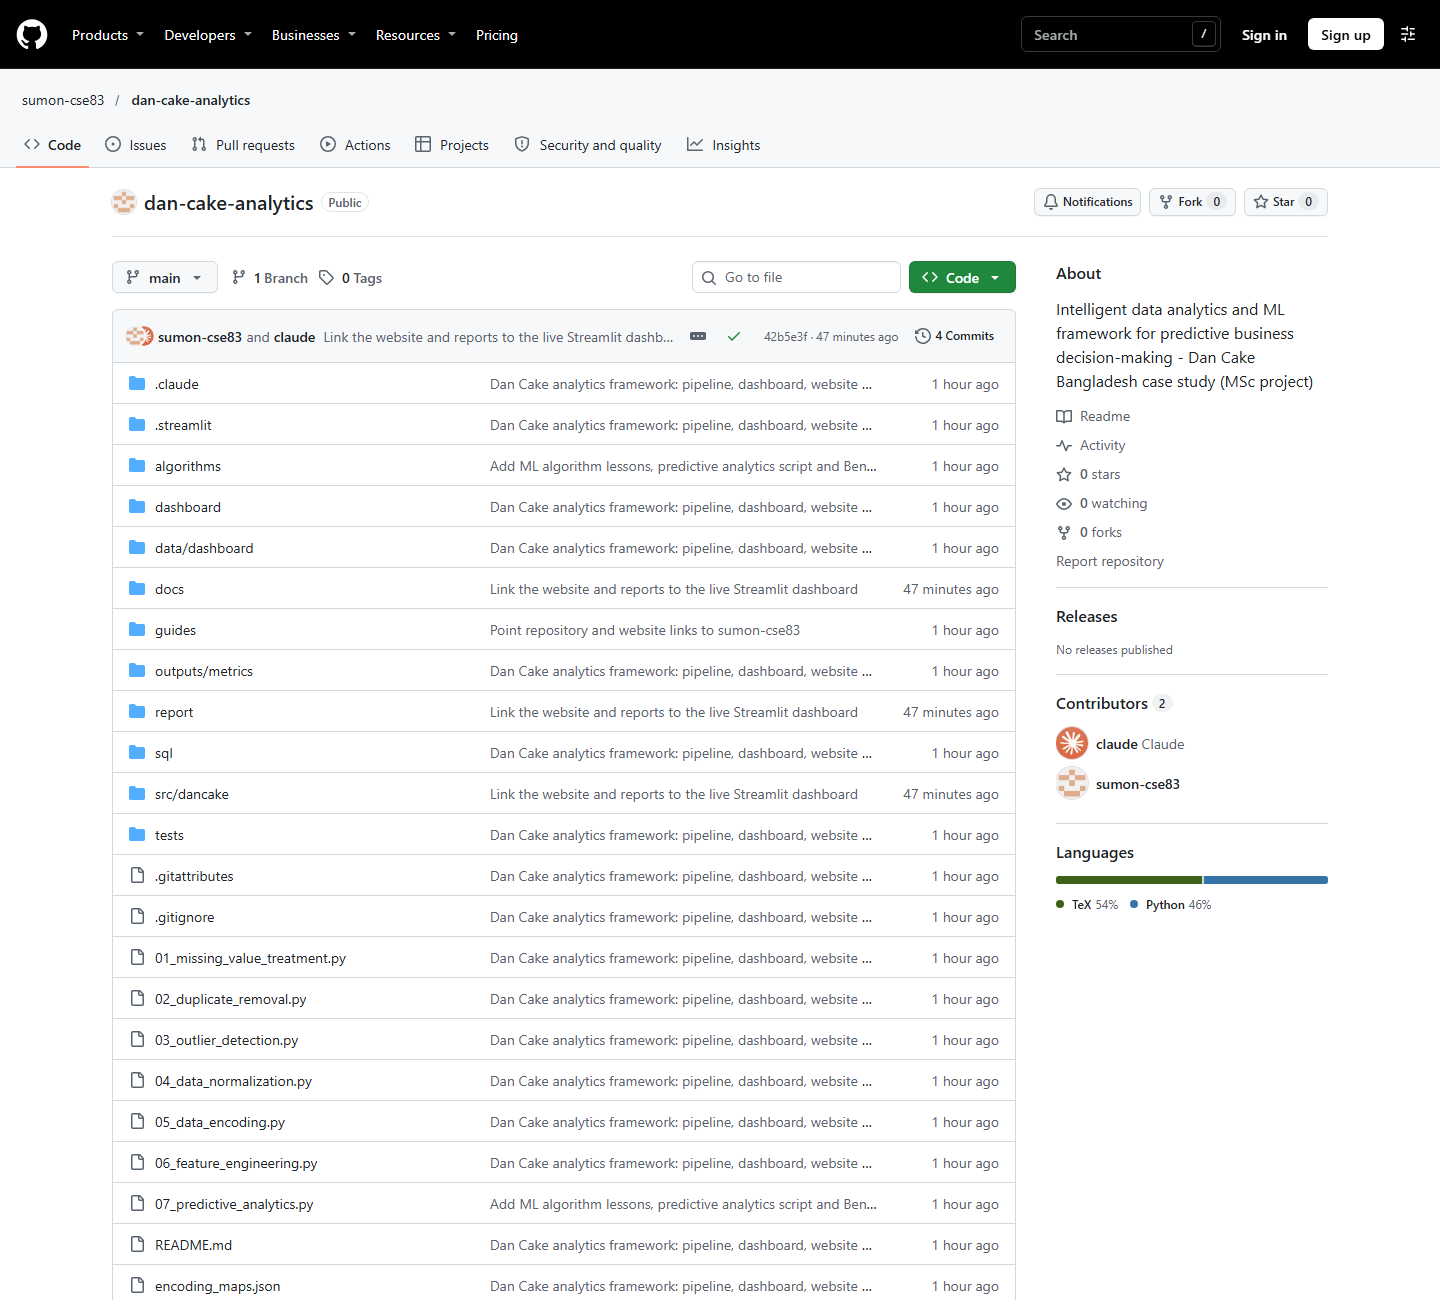
\includegraphics[width=\linewidth]{screens/github_repo}
\caption{Public GitHub repository holding the code, the dashboard data, the website and the report}\label{fig:github}
\end{figure}

If a custom domain name is bought later, it can be attached to GitHub Pages through a DNS \texttt{CNAME} record
without any change to the code. \Cref{app:reproduce} gives the step-by-step deployment procedure.

\section{Decision-support layer}
The final layer turns model outputs into recommendations. The module \texttt{insights.py} reads the metric
files and fills sentence templates with the current results. Every insight therefore stays up to date when new
data are processed, and none is typed by hand. The insights generated for this dataset are:

\begin{enumerate}[leftmargin=*,itemsep=4pt]
\item \textbf{Growth (What happened).} Net sales grew from 2020 to 2025 at 16.6\% a year, but units grew only 5.0\% a year; on average 11.3 percentage points of annual growth came from higher prices and mix, 5.0 from volume. \emph{Recommendation:} Track volume growth as a separate KPI; price-led growth is not sustainable indefinitely.
\item \textbf{Pricing (Why it happened).} After controlling for product, year and season, the estimated price elasticity of demand is +0.09 (95\% CI -0.28 to +0.46), i.e. not significantly different from zero. Discounts show no relationship with order size (Spearman rho = 0.001). \emph{Recommendation:} Review the discount budget (BDT 7.7 million over the period): discounts do not appear to buy volume.
\item \textbf{Seasonality (What happened).} December is the peak month (index 125, average month = 100) and February the weakest (86). The seasonal effect is statistically strong (Kruskal-Wallis p < 0.001). \emph{Recommendation:} Build stock and distributor capacity from October; schedule promotions and maintenance in February.
\item \textbf{Portfolio (What happened).} Muffin is the largest category (22.4\% of sales); the top 10 of 52 products deliver 38.5\% of revenue and 27 products form the 'A' class (80\% of sales). \emph{Recommendation:} Protect availability of A-class products first; review C-class products for rationalisation or repositioning.
\item \textbf{Portfolio (Segmentation).} Clustering finds 5 product segments; 'Premium \& gift packs' grows fastest (+7.8\% units a year, 33.3\% of sales). \emph{Recommendation:} Prioritise shelf space and marketing for 'Premium \& gift packs'.
\item \textbf{Market (What happened).} Dhaka alone generates 43.9\% of sales and Dhaka plus Chattogram 58.3\%. General Trade is the largest channel (45.6\%), while E-commerce is 5.9\%. \emph{Recommendation:} Reduce concentration risk by developing secondary cities and scaling E-commerce, which grows from a small base.
\item \textbf{Market (Segmentation).} The 'Emerging high-growth cells' segment (19 region-channel-customer cells, mainly Cumilla, Khulna, Mymensingh) is growing at +33.2\% a year, the fastest of the 4 market segments. \emph{Recommendation:} Allocate field-sales and digital-marketing effort to these emerging cells.
\item \textbf{Orders (Prediction).} Whether an order will be large ($\geq$ 10 units) is moderately predictable (best ROC-AUC 0.712, Logistic Regression); channel is by far the strongest driver: 48\% of distributor orders are large versus 8\% online. \emph{Recommendation:} Use the large-order score for delivery-vehicle and stock allocation, mainly at channel level.
\item \textbf{Forecast (What will happen).} The Support Vector Regression model forecasts next month's product demand with 11.1\% weighted error, 24\% lower RMSE than the seasonal-naive rule. Net sales for 2026-10 to 2027-09 are forecast at BDT 76.3 million (+12.1\% on the previous 12 months; 80\% range BDT 72.7 million - BDT 79.9 million). \emph{Recommendation:} Use the product-level forecast for the monthly production plan and the interval for safety stock.
\item \textbf{Risk (Anomalies).} 28 of 2,465 trading days were flagged as unusual. In a controlled test, rules plus Isolation Forest caught 91\% of 1,000 planted data errors. \emph{Recommendation:} Run the anomaly screen daily and investigate flagged days and orders before month-end reporting.
\end{enumerate}

Each insight is tagged by area and by the management question it answers. Each is paired with a concrete
action, so the dashboard serves as a \emph{decision-support system}, not merely a reporting tool.

\section{System evaluation}
The proposal asked for the system to be evaluated on predictive performance, usability, analytical usefulness,
visualisation quality and processing efficiency. \Cref{tab:syseval} summarises the evidence.

\begin{table}[htbp]\centering\small
\caption{Evaluation of the framework against the criteria in the proposal}\label{tab:syseval}
\begin{tabularx}{\linewidth}{@{}lX@{}}
\toprule
\textbf{Criterion} & \textbf{Evidence} \\ \midrule
Predictive performance & All ML forecasters beat naive baselines; best WAPE \BestRegWAPE\%; company-level MAPE \HWMAPE\%; classification ROC-AUC \ClsAUC (\cref{ch:models}); confirmed independently by the algorithm study (\cref{ch:algorithms}) \\
Analytical usefulness & Insights on growth quality, discount ineffectiveness, seasonality, concentration risk, segments and anomalies, each with a recommended action \\
Usability & One set of global filters; nine task-oriented pages with bookmarkable addresses; plain-language captions; downloadable forecasts; runs in any browser without installation \\
Visualisation quality & Principles of Few, Tufte and Knaflic: KPI cards, sorted bars, heat maps, intervals on forecasts, no 3-D or decorative charts, consistent palette \\
Processing efficiency & Data validation and cleaning of \NRows rows in under 20 seconds; warehouse load in \WarehouseSeconds s; full pipeline including model tuning in about 20 minutes on a standard laptop; dashboard data about 2 MB \\
Availability & Publicly deployed on free HTTPS platforms with automatic redeployment on every push (\cref{sec:deployment}) \\
Reproducibility & One command regenerates all data, models, figures, tables and numbers; fixed random seed; automated tests; version history on GitHub \\ \bottomrule
\end{tabularx}
\end{table}

A formal usability study with managers was beyond the time available. It is recommended as future work: a short
task-based test with a System Usability Scale questionnaire would complete the evaluation.

\chapter{Discussion}\label{ch:discussion}

\section{Answers to the research questions}

\paragraph{RQ1: How can data analytics improve business decision-making?}
The framework shows improvements at all three levels of analytics. At the \emph{descriptive} level, it replaces
manual spreadsheet consolidation with validated, reconciled KPIs that update with one command. At the
\emph{diagnostic} level, it reveals relationships that simple reports would miss. Growth is mostly price- and
mix-led. Discounts are not associated with larger orders. Order size depends on the channel, not the customer
type. At the \emph{predictive} level, it provides product-level forecasts with quantified uncertainty. Each of
these changes a concrete decision: discount budgets, sales-force allocation, production plans and logistics
capacity.

\paragraph{RQ2: Which preprocessing techniques are most effective?}
Three techniques proved most valuable. The first is \emph{deriving} missing values from accounting identities,
which gives exact restoration and should always be tried before statistical imputation. The second is
\emph{robust, group-wise outlier detection} (a per-product IQR on the log scale), which respects skewed
distributions and different product scales. Combined with the policy of flagging rather than deleting unusual
values, it keeps genuine bulk orders. The third is \emph{leakage-safe feature engineering}, in which history
features are shifted before rolling and every learned parameter is fitted on training data only. Robust
methods were preferable to normal-theory methods throughout, because the business variables are highly skewed.

\paragraph{RQ3: Which algorithm performs best?}
No single algorithm is best for every problem, and the margins between good models are small. For one-month-ahead
product demand, \BestReg was most accurate. \BestRec was most robust in the multi-step setting. At the company
level, the classical Holt--Winters model beat all machine-learning alternatives. For classification, logistic
regression matched the tree ensembles. This pattern agrees with \citet{makridakis2018}. Good features, a sound
validation design and benchmarking matter more than the choice of algorithm. A combined approach, with
statistical totals reconciled to machine-learned product mixes, is the most useful in practice. The
algorithm-level study in \cref{ch:algorithms} reached the same conclusion with independent code and a simpler
feature set. There, \AlgRegBest had the lowest monthly error (MAE \AlgRegBestMAE units), but linear regression
(\AlgLinMAE) and the random forest (\AlgRFMAE) were within a few units of it, and the seven classifiers spanned
only \AlgClsWorstAUC to \AlgClsBestAUC in ROC-AUC. Because the exact ranking of the leading models changes with
the features and tuning, the choice among them should favour simplicity and explainability.

\paragraph{RQ4: What patterns exist in the historical data?}
Strong year-end seasonality peaks in \PeakMonth. Growth is steady but price-driven, and demand is
price-inelastic. Revenue is geographically concentrated in Dhaka and Chattogram, and the portfolio is
concentrated in about ten products. Order size differs strongly by channel. Discounts have no detectable volume
effect, and weekday effects are absent. Segmentation adds a portfolio view (premium and gift packs, core family
packs, value single-serves and niche lines) and a market view (core retail, bulk distribution, online and
regional, emerging high-growth).

\paragraph{RQ5: How accurately can the future be predicted?}
Monthly demand per product can be forecast with a weighted error of about \BestRegWAPE\% one month ahead and
about \BestRecWAPE\% up to 21 months ahead. Company-level monthly units can be forecast with an error of about
\HWMAPE\%. Whether an individual order will be large is only moderately predictable (ROC-AUC \ClsAUC). The
limit lies in the information available, not in the models.

\paragraph{RQ6: How should results be presented to managers?}
Through an interactive dashboard organised around the management questions. It should have global filters,
KPI cards and simple, sorted charts; it should always show uncertainty for forecasts; and it should state
insights in plain language, each with an action. Publishing the dashboard and a summary website on free
platforms removes cost and installation barriers. In this project both are live (\cref{tab:links}), every page
has its own shareable address, and continuous deployment means that managers always see the latest results
without any action on their part.

\paragraph{RQ7: How much does predictive analytics add to historical reporting?}
A historical report can at best repeat last year's pattern, which is the seasonal-naive rule. The
machine-learning forecast reduces its error by \GainVsSNaive\%. Put differently, a planner using last year's
figures would make errors about \SNaiveWAPE\% of volume in each product-month, compared with \BestRegWAPE\% for
the framework. Prediction intervals add information that historical reporting cannot provide at all: how much
safety stock is needed.

\section{Managerial implications}
\begin{itemize}
  \item \textbf{Pricing and promotions.} Demand is inelastic and discounts do not raise order size. The discount
        budget of about \BDT\DiscountCost million over the period should be reviewed. Controlled experiments
        (A/B promotions) should establish whether targeted promotions pay off.
  \item \textbf{Volume growth.} Because growth relies on price, volume should become a separately tracked KPI,
        with growth initiatives in under-penetrated regions and in E-commerce.
  \item \textbf{Seasonal planning.} Production and distributor stock should be built from October for the
        \PeakMonth peak. February is the natural window for maintenance and promotions.
  \item \textbf{Portfolio.} The A-class products deserve the highest service levels. C-class products are
        candidates for review.
  \item \textbf{Logistics.} Large orders are concentrated in the distributor channel and in particular regions.
        Vehicle and stock allocation can be planned at that level.
  \item \textbf{Control.} A daily anomaly screen improves data quality and detects operational problems early.
\end{itemize}

\section{Limitations}\label{sec:limitations}
\begin{itemize}
  \item \textbf{Data provenance and realism.} The dataset is very clean: it has no missing values, its
        accounting identities hold exactly, and order size is almost independent of customer type, discount and
        product. Real operational data are usually messier. The pipeline was therefore tested on deliberately
        damaged copies, but conclusions about customer behaviour should be validated on further company data
        before they are acted on. The exact source and collection process of the dataset should be documented
        alongside this report.
  \item \textbf{Missing drivers.} No data were available on marketing spend, competitor prices, stock-outs,
        weather or holidays. Including them would probably improve both forecasting and classification.
  \item \textbf{Observational elasticity.} The elasticity estimate rests on list-price variation over time, not
        on randomised experiments. Prices changed by small amounts, so elasticity outside the observed range is
        unknown.
  \item \textbf{Future conditions.} All forecasts assume that past patterns continue. Structural breaks, such as
        a new competitor or an economic shock, would reduce accuracy.
  \item \textbf{Scope of evaluation.} The dashboard has not yet been evaluated with real managers. Deep-learning
        models were not explored, because the panel (52 series of 81 months) is too small to justify them.
\end{itemize}

\section{Reflection on the methodology}
Strict time-ordered evaluation with benchmarks was the most important methodological decision. Random
cross-validation would have produced flattering but misleading accuracy figures. Generating every reported
number from code turned out to be valuable as well: analyses were re-run many times as the work progressed, and
the report always remained consistent. Running a second, independent modelling study (\cref{ch:algorithms})
proved a cheap and effective way to test whether the conclusions depended on one implementation. Both practices
are recommended for future projects of this kind.

\chapter{Conclusion and Future Work}\label{ch:conclusion}

\section{Conclusion}
This project set out to design and develop an intelligent data analytics and machine learning framework that
transforms raw business data into actionable insights and predictive information. All seven objectives were
met. A dataset of \NRows transactions was validated, cleaned and stored in a dimensional data store (O1, O2).
Exploratory and inferential analysis revealed price-led growth, inelastic demand, ineffective discounts, strong
year-end seasonality and high geographical and portfolio concentration (O3). Seven regression and seven
classification algorithms, three clustering methods, statistical forecasting models and two anomaly detectors
were developed and compared under a strict time-ordered protocol (O4). Each of the nine algorithms named in the
proposal was also studied on its own, which explained its behaviour and independently confirmed the results.
The results are delivered through a nine-page interactive dashboard and a project website that are publicly
deployed free of charge, with continuous deployment from GitHub (O5), and through automatically generated
insights and recommendations (O6). The framework's predictive performance, usefulness, efficiency and reproducibility were
evaluated (O7).

The central conclusion is that the greatest value comes from \emph{integration} and \emph{discipline}, not from
the most complex algorithm. Clean and validated data, leakage-safe features, honest benchmarks and clear
communication turned simple and well-understood models into reliable decision support. The best
product-level forecasts cut the error of ``same as last year'' planning by \GainVsSNaive\%. Classical and
machine-learning methods worked best together. The organisation can thus move from describing the past to
anticipating the future, answering \emph{what happened}, \emph{why} and \emph{what next} within one system.

\section{Future work}
\begin{itemize}
  \item \textbf{Richer data:} add promotions, marketing spend, competitor prices, inventory and stock-outs,
        public holidays (Eid, Pohela Boishakh) and weather, and integrate them through APIs.
  \item \textbf{Real-time analytics and alerts:} schedule the pipeline daily in the cloud and send anomaly and
        forecast-deviation alerts by e-mail or messaging.
  \item \textbf{MLOps:} version data and models, monitor forecast accuracy over time and retrain automatically
        when performance drifts.
  \item \textbf{Prescriptive analytics:} optimise production quantities and distributor allocations under
        capacity constraints, using the forecast intervals.
  \item \textbf{Causal evaluation of promotions:} run controlled promotion experiments to measure the true
        effect of discounts.
  \item \textbf{Advanced models:} hierarchical reconciliation across product, region and channel, and global
        deep-learning forecasters once longer and more granular histories are available.
  \item \textbf{Generative-AI assistant:} let managers ask questions in natural language (for example,
        ``why did Rangpur sales fall in March?'') and receive answers grounded in the framework's data and metrics.
  \item \textbf{Usability study:} evaluate the dashboard with managers using task-based tests and the System
        Usability Scale.
\end{itemize}


\bibliographystyle{plainnat}
\bibliography{references}

\appendix
\chapter{Data Dictionary}\label{app:dictionary}
\begin{table}[htbp]\centering\footnotesize
\caption{Data dictionary of the transaction dataset}\label{tab:dictionary}
\begin{tabularx}{\linewidth}{@{}llX@{}}
\toprule
\textbf{Column} & \textbf{Type} & \textbf{Description} \\ \midrule
Transaction\_ID & text & Unique transaction identifier (e.g.\ DC2020000000) \\
Date & date & Transaction date (dd-mm-yy) \\
Year, Month, Month\_Name, Quarter & integer/text & Calendar attributes derived from the date \\
Product\_ID, Product\_Name & text & Product code and name (\NProducts products) \\
Category & text & Product category (13 categories) \\
Pack\_Size & text & Pack size, e.g.\ 30g, 27--30g, 30g x 12, 5 pcs \\
Product\_Launch\_Year & integer & Year the product was introduced \\
Observed\_Price\_BDT & integer & Printed maximum retail price \\
List\_Price\_BDT & integer & Company list price for the year \\
Market\_Price\_BDT & decimal & Transaction price before discount \\
Discount\_\% & decimal & Discount percentage \\
Unit\_Selling\_Price\_BDT & decimal & Price per unit after discount \\
Quantity & integer & Units sold \\
Gross\_Sales\_BDT & decimal & Quantity $\times$ market price \\
Discount\_BDT & decimal & Discount amount \\
Net\_Sales\_BDT & decimal & Gross sales $-$ discount \\
Region & text & One of 11 regions of Bangladesh \\
Channel & text & General Trade, Modern Trade, Distributor, E-commerce \\
Customer\_Type & text & Retailer, Super Shop, Distributor, Corporate, Online Customer \\ \bottomrule
\end{tabularx}
\end{table}

\chapter{Tuned Hyper-parameters}\label{app:hyper}
\begin{table}[htbp]
\centering
\footnotesize
\caption{Hyper-parameters selected by randomised search with expanding-window validation (demand forecasting)}
\label{tab:hyper}
\begin{adjustbox}{max width=\linewidth}
\begin{tabular}{l>{\raggedright\arraybackslash}p{10cm}}
\toprule
\textbf{Model} & \textbf{Selected hyper-parameters} \\
\midrule
Linear Regression & none (closed form) \\
Decision Tree & max\_depth=10, min\_samples\_leaf=40 \\
Random Forest & max\_depth=None, max\_features=0.33, min\_samples\_leaf=2, n\_estimators=500 \\
Gradient Boosting & learning\_rate=0.05, max\_depth=2, n\_estimators=200, subsample=1.0 \\
XGBoost & colsample\_bytree=0.6, learning\_rate=0.02, max\_depth=3, min\_child\_weight=10, n\_estimators=600, reg\_lambda=1, subsample=0.9 \\
K-Nearest Neighbors & n\_neighbors=20, weights=distance \\
Support Vector Regression & C=0.3, epsilon=0.05, gamma=0.01 \\
\bottomrule
\end{tabular}
\end{adjustbox}
\end{table}

\chapter{Example SQL Queries}\label{app:sql}
The following queries run on the star schema (\cref{fig:star}) and reproduce key figures of \cref{ch:eda}
directly in SQL. They can also be used as the data source of a Power BI report.
\lstinputlisting[language=SQL]{sql/kpi_queries.sql}

\chapter{Reproducing and Deploying the Project}\label{app:reproduce}
\section{Project structure}
\begin{lstlisting}
dan_cake_project/
  run_pipeline.py          one command for the whole framework
  src/dancake/             config, data, eda, features, forecasting, classification,
                           clustering, anomaly, insights, export, website
  dashboard/app.py         Streamlit dashboard
  data/  processed/ warehouse/ dashboard/   generated data
  outputs/ metrics/ tables/ models/          generated results
  report/  main.tex, chapters/, figures/, tables/, generated/
  docs/                    project website (GitHub Pages)
  sql/  tests/  guides/
\end{lstlisting}

\section{Running locally}
\begin{lstlisting}[language=bash]
python -m venv .venv
.venv\Scripts\activate            # Windows  (source .venv/bin/activate on macOS/Linux)
pip install -r requirements.txt
python run_pipeline.py            # about 20 minutes
python -m pytest tests            # automated tests
streamlit run dashboard/app.py    # open http://localhost:8501
\end{lstlisting}

\section{Free deployment}
\begin{enumerate}
  \item Create a free GitHub account and a public repository; push the project (the raw CSV is excluded by
        \texttt{.gitignore}; the small dashboard data are included).
  \item \textbf{Dashboard:} sign in to Streamlit Community Cloud with GitHub, choose \emph{New app}, select the
        repository, branch \texttt{main} and file \texttt{dashboard/app.py}, then deploy. The app receives an
        address ending in \texttt{.streamlit.app}.
  \item \textbf{Website:} in the repository settings, open \emph{Pages}, choose \emph{Deploy from a branch},
        branch \texttt{main}, folder \texttt{/docs}. The site appears at \path{https://<user>.github.io/<repo>}.
  \item Regenerate the website with the real links (run inside \texttt{src}), then commit and push:
\begin{lstlisting}[language=bash]
python -m dancake.website --dashboard-url <app url> \
                          --repo-url <repo url>
\end{lstlisting}
\end{enumerate}

\section{Re-using the framework for another project}
Only \texttt{src/dancake/config.py} (paths, column names, train/test dates) and the column lists in the
feature functions need to change for a new sales dataset. The structure, namely validation, cleaning,
warehouse, EDA, leakage-safe features, benchmarked models, dashboard, insights and generated report, transfers
unchanged to other domains such as inventory, finance or customer analytics.


\end{document}
